\documentclass[11pt]{book}

\usepackage[htt]{hyphenat}
\usepackage{multind}
\usepackage[pdftitle={POY 4.0 Documentation},pdfauthor={Andres Varon et. al.},
pdfkeywords={phylogenetic analysis, direct optimization, POY}]{hyperref}
\usepackage{color}
\usepackage{xspace}
\usepackage{framed}
\usepackage{graphicx}
\usepackage{rotating} % to create landscape pages
%\usepackage{makeidx}

%Indexes
\makeindex{general}
\makeindex{poy3}

\newlength\sidebar
\newlength\envrule
\newlength\envborder
\newlength\boxwidth

\setlength\sidebar{1.5mm}
\setlength\envrule{0.4pt}
\setlength\envborder{2.5mm}

\definecolor{exampleborder}{rgb}{0,0,.7}
\definecolor{examplebg}{rgb}{.9,.9,1}
\definecolor{shadecolor}{rgb}{.9,.9,1}
\definecolor{statementborder}{rgb}{.9,0,0}
\definecolor{statementbg}{rgb}{1,.9,.9}

\newsavebox\envbox
\newlength\notelength

\newenvironment{statement}[1][NOTE]{
% Default statement has no title %ilya: Statement is used for NOTES
\SpecialEnv{#1}{statementborder}{statementbg}{statementborder}{}%
}{%
\endSpecialEnv}

\def\Empty{}

% #1 title (if any)
% #2 sidebar (and title bg) color
% #3 background color
% #4 border color (or null for no border)
% #5 \enspace

	\newenvironment{SpecialEnv}[5]{%
	\par
	\def\EnvSideC{#2}% To use later (in end)
	\def\EnvBackgroundC{#3}%
	\def\EnvFrameC{#4}% 
	\flushleft

%\setlength\leftskip{-\sidebar}%
%\addtolength\leftskip{-\envborder}%
\noindent \nobreak
% Check if title is null:
\ifx\delimiter#1\delimiter\else
% If a title is specified, then typeset it in reverse color
\colorbox{\EnvSideC}{%
%\hspace{-\leftskip}% usually positive
%\hspace{-\fboxsep}%
\footnotesize\sffamily\bfseries\textcolor{white}{#1}%
%\hspace{\envborder}}%
}
\par\nobreak
\setlength\parskip{-0.2pt}% Tiny overlap to counter pixel round-off errors
\nointerlineskip 
\fi

% Make side-bar
\textcolor{\EnvSideC}{\vrule width\sidebar}%
% collect body in \envbox:
\begin{lrbox}\envbox 
\setlength{\boxwidth}{\linewidth}
\settowidth{\notelength}{NOT}
\addtolength{\boxwidth}{-1\notelength}
\addtolength{\boxwidth}{-1\sidebar}
\addtolength{\boxwidth}{-1\envborder}
\begin{minipage}[l]{\boxwidth}%

% insert counter, if any:
\ifx\delimiter#5\delimiter\else
%\theexample.\enspace
\fi
\ignorespaces
}{\par
\end{minipage}
\end{lrbox}%
% body is collected. Add background color
\setlength\fboxsep\envborder
\ifx\EnvFrameC\Empty % no frame
\colorbox{\EnvBackgroundC}{\usebox\envbox}%
\else % frame
\setlength\fboxrule\envrule
\addtolength\fboxsep{-\envrule}%
\fcolorbox{\EnvFrameC}{\EnvBackgroundC}{\usebox\envbox}%
\fi
\nobreak \hspace{-2\envborder}\null
\endflushleft
}


\newenvironment{poyexamples}{ \subsubsection{Examples} \begin{itemize}}{\end{itemize}}
% We define a command environment for new command definitions, and store
% whatever command we are dealing with in the @commandname macro. Inside a
% command we can specify the defaults, the syntax, and the arguments to be used.
\newenvironment{command}[2]{
    \def\tmpa{}
    \def\tmpb{#2}
    \def\@commandname{#1}
    \subsection{#1}\index{general}{#1}
    \ifx\tmpa\tmpb 
        \label{comm:#1} 
    \else 
        \label{comm:#2} 
    \fi}
    {}
% Syntax definition. We use the name of the command as stured in @commandname
\newcommand{\syntax}{\subsubsection{Syntax} \@commandname} 
\newcommand{\atsymbol}{@}

% We need to choose properly if we need to open a description or not inside
% an argument or argument group environment. We will use these two variables
% to keep the proper value to be used on each point.
\def\opendescription{\begin{description}}
\def\closedescription{}

% We define a pair of commands to initialize and finalize a description list 
% and set the necessary values of opendescription and closedescription.
\newcommand{\initdescription}{
    \def\closedescription{\end{description}}
    \opendescription
    \def\opendescription{}
}
\newcommand{\finishdescription}{
    \closedescription
    \def\closedescription{}
    \def\opendescription{\begin{description}}
}

% A variable to store a prefix for argument definitions, usually a colon.
\def\argprefix{} 

\newenvironment{script}{\begin{verbatim}}{\end{verbatim}}
\newcommand{\poyexample}[2]{\item \commandstyle{#1} \\#2}
\newcommand{\commandstyle}[1]{\texttt{#1}}
\newcommand{\poycommand}[1]{\commandstyle{#1}}

% Argument specifications
\newcommand{\poyargument}[1]{\commandstyle{#1}}
\newcommand{\obligatory}[1]{\commandstyle{\argprefix#1}}
\newcommand{\optional}[1]{\commandstyle{[\argprefix#1]}}
\newenvironment{arguments} {\subsubsection{Arguments}}{ \finishdescription }
\newenvironment{argumentgroup}[2]{\paragraph{#1} #2}{ \finishdescription }
\newcommand{\argumentdefinition}[4]{
    % Check if we are inside an itemize environment or not, if not, start
    % it.
    \initdescription
    % We will check if the second argument is empty; if so, we don't need
    % the add the : prefix for the argument's value.
    \def\tmpa{}
    \def\tmpb{#2}
    \def\tmpc{#4}
    \index{general}{#1}
    \index{general}{\@commandname!#1}
    \ifx\tmpa\tmpb
        \item[\poyargument{#1}]
            \ifx\tmpa\tmpc
                \label{comm:#1}
            \else
                \label{comm:#4}
            \fi
                #3
    \else
        \def\argprefix{:}
        \item[\poyargument{#1#2}]
            \ifx\tmpa\tmpc
                \label{comm:#1}
            \else
                \label{comm:#4}
            \fi
            #3
    \fi
    \def\argprefix{}
    }

\newenvironment{poydescription}{\subsubsection{Description}}{}

% The primitive types of a POY script.
\newcommand{\poystring}{\commandstyle{STRING}\xspace}
\newcommand{\poyfloat}{\commandstyle{FLOAT}\xspace}
\newcommand{\poyint}{\commandstyle{INTEGER}\xspace}
\newcommand{\poybool}{\commandstyle{BOOL}\xspace}
\newcommand{\poylident}{\commandstyle{LIDENT}\xspace}

\newcommand{\poydefaults}[2]{\subsubsection{Defaults} \commandstyle{\@commandname(#1)} #2}

\newenvironment{poyalso}{\subsubsection{See also}
\begin{itemize}}{\end{itemize}}

% Cross References
\newcommand{\cross}[1]{\item \commandstyle{#1} (Section~\ref{comm:#1})}
\newcommand{\ncross}[2]{\item \commandstyle{#1} (Section~\ref{comm:#2})}

\newcommand{\ccross}[1]{\commandstyle{#1} (Section~\ref{comm:#1})}
\newcommand{\nccross}[2]{\commandstyle{#1} (Section~\ref{comm:#2})}

% The typesetting of POY
\newcommand{\poy}{\commandstyle{POY4}\xspace}
\newcommand{\poyv}{\commandstyle{POY4}\xspace} % poyv stands for "poy version 4"

% Using same footnotes multiple times (used for authorship)
\newcommand{\footnoteremember}[2]{
  \footnote{#2}
  \newcounter{#1}
  \setcounter{#1}{\value{footnote}}
}
\newcommand{\footnoterecall}[1]{
  \footnotemark[\value{#1}]
}

% Hyphenations
\hyphenation{mo-le-cu-lar an-aly-ses an-aly-sis au-to-ma-ti-cally ho-mo-lo-gy chro-mo-so-me chro-mo-so-me-le-vel op-ti-mi-za-tion}

\makeatletter
\def\thickhrulefill{\leavevmode \leaders \hrule height 1pt\hfill \kern \z@}
\renewcommand{\maketitle}{\begin{titlepage}%
    \let\footnotesize\small
    \let\footnoterule\relax
    \parindent \z@
    \reset@font
    \null
    \vskip 50\p@
    \begin{center}
      {{\huge \texttt{POY} 4.0 R.C.}
      \par 
      \vskip \baselineskip
      \hrule height 1pt 
      \par 
      \vskip \baselineskip
      Program Documentation 
      \par
      \small Version 4.0.\buildnumber }\par
    \end{center}
    \vskip 85\p@
    \begin{flushright}
      \@author \par
    \end{flushright}
    \vskip 85\p@
    \begin{center}
    
\includegraphics[width=\textwidth]{figures/amnhlogoblue2.pdf}
    \end{center}
    \vfil
    \null
  \end{titlepage}%
  \setcounter{footnote}{0}%
}
\makeatother

\newcommand{\smallbuildnumber}{5.0}\newcommand{\buildnumber}{Black Sabbath Development build 2a12624f96c4}


\author{\textbf{Program and Documentation} \\ Andr\'es Var\'on \\ Le Sy Vinh \\
Illya Bomash \\ Ward C. Wheeler \\ \bigskip \textbf{Documentation} \\ Ilya T\"emkin \\ Megan Cevasco \\ Kurt M. Pickett \\ Juli\'an Faivovich \\ Taran Grant \\ William Leo Smith}


%%%%%%%%%%%%%%%%%%%%%%%%%
%	BODY TEXT OF THE DOCUMENT     
%%%%%%%%%%%%%%%%%%%%%%%%%

\begin{document}

\maketitle

\thispagestyle{empty}

\vspace*{5.5cm}

\begin{flushleft}
    \small
{\it
Andr\'es Var\'on}\\
Division of Invertebrate Zoology, American Museum of Natural History, New York, NY, U.S.A. \\
Computer Science Department, The Graduate School and University Center, The City University of New York, NY, U.S.A.  \\
\smallskip 
{\it
Le Sy Vinh\\
Ward C. Wheeler\\
Ilya T\"emkin \\
Megan Cevasco \\
}
Division of Invertebrate Zoology, American Museum of Natural History, New York, NY, U.S.A.\\
\smallskip 
{\it
Kurt M. Pickett}\\
Department of Biology, University of Vermont, Berlington, VT, U.S.A.\\
\smallskip
{\it
Juli\'an Faivovich}\\
Departamento de Zoologia, Instituto de Bioci\^encias, Universidade Estadual Paulista, Brasil\\
\smallskip
{\it
Taran Grant}\\
Faculdade de Bioci\^encias, Pontif�cia Universidade Cat\'olica do Rio Grande do Sul (PUCRS), Brasil\\
\smallskip
{\it
William Leo Smith}\\
Department of Zoology, The Field Museum of Natural History, Chicago, IL, U.S.A.\\

\vspace*{0.5cm}
The American Museum of Natural History\\
\copyright 2007 by The American Museum of Natural History \\
All rights reserved. Published 2007

\vspace*{0.5cm}

\emph{Var\'on, A., L. S. Vinh, I. Bomash, W. C. Wheeler.} 2007.
\texttt{POY} 4.0.\buildnumber\ R.C. New York, American Museum of
Natural History. Documentation by Var\'on, A., L. S. Vinh, I. Bomash,
W. Wheeler, I. T\"emkin, M. Cevasco, K. M. Pickett, J. Faivovich, T. Grant, and
W. L. Smith. \url{http://research.amnh.org/scicomp/projects/poy.php}

\vspace*{0.5cm}

Available online at
\url{http://research.amnh.org/scicomp/projects/poy.php}
and
\url{http://code.google.com/p/poy4/}

\end{flushleft}

\tableofcontents

\chapter{What is \poy}

\poy is a flexible, multi-platform program for phylogenetic analysis of molecular and other data. %under various optimality criteria.
An essential feature of \poy is that it implements the concept of dynamic homology \cite{wheeler2001a, wheeler2001} allowing optimization of unaligned sequences. \poy offers flexibility for designing heuristic search strategies and implements an array of algorithms including multiple random addition sequence, swapping, tree fusing, tree drifting, and ratcheting. As output, \poy generates a comprehensive character diagnosis, graphical representations of cladograms and their user-specified consensus, support values, and implied alignments. \poy provides a unified approach to co-optimizing different types of data, such as morphological and molecular sequence data. In addition, \poy can analyze entire chromosomes and genomes, taking into account large-scale genomic events (translocations, inversions, and duplications).

%Currently \poy is beta software, and therefore it has some known glitches. Most
%of them will be worked out in the following months, and updated versions will be
%available on the program's webpage as we produce them. Our current schedule of
%work expect to have a final official version of the parsimony components of the
%program and a release of the beta components of the maximum
%likelihood components in mid may of 2007.

\section{The structure of \poy documentation}
This first chapter, \emph{\poy Quick Start}, will get you started using \poy. The first few sections are intended to provide detailed instructions on how to obtain and install \poy, introduce the user to the program's two working environments, the \emph{Graphical User Interface} and the \emph{Interactive Console}. These sections also show how to initiate a \poy session and point to the various resources to obtain further assistance. Subsequent sections build on that knowledge and give step-by-step examples on how to conduct a basic analysis and visualize the results. The second chapter, \emph{\poy Commands}, describes \poy commands and their valid syntax. It also includes examples of simple operations for every command. The third chapter discusses the heuristic procedures used in \poy. Their understanding helps creating building efficient search strategies. More advanced operations are described in the fourth chapter, \emph{\poy Tutorials}. In addition to the general index, this document contains a \emph{\texttt{POY3.0} Command Line Index}, intended to provide a link between the commands used in \texttt{POY3} and the commands used in \poy. 

\chapter{\poy Quick Start}

\section{Requirements: software and hardware}

\subsection{Software}
\poy is a platform-independent, open-source program that can be
compiled for many operating systems and hardware configurations,
including Mac OSX, Microsoft Windows and Linux. %\poy \emph{binaries}
%\index{general}{binaries} (compiled application file) is the only
piece of software necessary to run \poy%1.0.  The intuitive
\emph{Graphical User Interface} of \poy provides the functionality
for running analyses using pull-down menus and field selections,
as well as creating and running \poy scripts. Some utility programs
(such as Notepad and Ghostscript for Windows, TextEdit for Mac, or
Nano for Linux), can help preparing \poy scripts and formatting
data files, while others (such as Adobe Acrobat) can facilitate
viewing the graphical output in PDF (Portable Document Format).

\subsection{Hardware}
\poy runs on a variety of computers from laptops and desktops to
clusters of various sizes and symmetric multiprocessing hardware.
There are no particular requirements for disk space, but XML and
diagnosis report files can be large.

\section{Obtaining and installing \poy}
\subsection{Installing from the binaries}
\poy installers for Windows and Mac OSX, source code, and documentation
in PDF format are available from the \poy download website at the
Computational Sciences site of the American Museum of Natural
History:

\begin{center}
\url{http://www.amnh.org/our-research/computational-sciences/research/projects/systematic-biology/poy}
\end{center}

The latest source code can also be obtained from \poy Google Group website:
\begin{center}
\url{http://code.google.com/p/poy/source}
\end{center}

The following detailed step-by-step instructions will guide you
through downloading and installing \poy \emph{binaries} for various
platforms.

\begin{flushleft}
\begin{minipage}[c]{0.074\textwidth}

\includegraphics[width=\textwidth]{doc/figures/figlogowindows.jpg}
\end{minipage}
\,
\begin{minipage}[t]{0.88\textwidth}
\subsubsection*{Windows}
\end{minipage}


\begin{itemize}
\item
Download the
\href{http://www.amnh.org/our-research/computational-sciences/research/projects/systematic-biology/poy/download}
{\emph poy5} folder to the desktop by selecting the \emph{Windows} 
download link.

\item Open the \emph{POY\_version.zip}.  You will need Administrator
privileges to install the application.  Extract the zip file to
install in the desired location and execute the \emph{poy.exe} file.
If you have Windows XP SP2, Windows Vista or Windows 7 and possess
more than one core or processor, you can take advantage of this
processing power \ by installing the parallel components
\href{http://www.mpich.org}{MPICH2}.

[Note: The \poy developers encountered no problems when using MPICH2 3.0.2.]
\end{itemize}

\begin{minipage}[c]{0.074\textwidth}

\includegraphics[width=\textwidth]{doc/figures/figlogomac.jpg}
\end{minipage}
\,
\begin{minipage}[t]{0.88\textwidth}
\subsubsection*{Mac OSX}
\end{minipage}
\begin{itemize}
\item Download
\href{http://www.amnh.org/our-research/computational-sciences/research/projects/systematic-biology/poy/download}
{\emph{poy-buildXXXX.dmg}} disk image to the desktop. The complete
installation of the Mac OSX version of \poy includes MPICH2 1.4.1,
which is used to communicate processes during parallel execution.
\item Drag the \poy application from the disk \emph{poy5} and drop
it into the \emph{Applications} folder on the hard drive.

[Note: During the first execution in parallel you may be asked by
the Firewall to unblock \poy and MPICH.  This is necessary for
successful execution of the program.] \end{itemize}

\begin{minipage}[c]{0.074\textwidth}

\includegraphics[width=\textwidth]{doc/figures/figlogolinux.jpg}
\end{minipage}
\,
\begin{minipage}[t]{0.88\textwidth}
\subsubsection*{Linux}
\end{minipage}
\begin{itemize}
\item  No binaries are available for the Linux operating system.
The user should compile \poy directly from the source (see
Section~\ref{Compilingfromsource}).  \end{itemize}

\end{flushleft}

\subsection{Compiling from the source}
\label{Compilingfromsource}

For the majority of users, downloading the binaries from the \poy
download site will suffice.  However, in some cases it may be %either
necessary: analysis of chromosomal and genomic data (\textgreater16383
%nucleotides long); \hl{likelihood analyses}; or if working with
large alphabets (\textgreater255 elements), or% desirable --- user
preference for working in a command-line environment or running
\poy analyses in parallel (in the case of Linux machines or on a
cluster computer), or necessary (in the case of Linux users) ---
to compile \poy directly from the source code (see Table
\ref{InterfaceGuide} and \ref{ParallelizationGuide}).  If the user
chooses to compile, it is advisable to check out the various
configuration options that can be found in {\tt ./configure --help}
of the \texttt {src} directory. \\ \\ In order to compile \poy the
following tools are required:

\begin{enumerate}
\item The \href{http://www.gnu.org/software/make/}{GNU Make 3.8} utility. 
\item OCaml \href{http://www.ocaml.org}{version 3.11.2.} or later. 
\item A {\bf C} compiler, for example \href{http://gcc.gnu.org/} 
{The GNU Compiler Collection.}
\item \href{http://www.zlib.net}{The zlib compression library.}
\item The Linear Algebra PACKage \href {http://www.netlib.org/lapack/}
{LAPACK} must be installed in order to use the likelihood option.
\item The \href{http://www.gnu.org/s/ncurses} {ncurses library} 
is necessary to compile the default interface, i.e. \emph{ncurses} 
or the \emph{Interactive Console}. If this library is not available, 
the \emph{flat} interface will be compiled instead.
\item The Message Passing Interface \href{http://www-unix.mcs.anl.gov/mpi/}
{MPICH2}, which is used to communicate processes during parallel execution.
%  the complete installation includes MPICH2 \hl{1.06 p1}. MPICH is used to 
%communicate processes during parallel execution (if you didn't know what it 
%is you most likely don't have it), select the custom installation option 
%and remove that component. During the first execution in parallel you 
%will be asked by the Windows Firewall to %unblock \poy and MPICH: 
%this is necessary for the successful execution of the program.
\item The \href{http://www.tsp.gatech.edu/concorde/}{Concorde Package}, 
which includes TSP median solvers used in the calculation of 
chromosome and genome rearrangements. 
\end{enumerate}
Download, ungzip and untar the
\href{http://www.amnh.org/our-research/computational-sciences/research/projects/systematic-biology/poy/download}
{\poy source code}.  In a terminal window, change directories to the path of this 
uncompressed directory. In order to compile under default setting, 
working in the source directory (\texttt{src}), type:

\begin{verbatim}
./configure
make
make install
\end{verbatim}

To \texttt{make install}, it may be necessary to do this as the
root user using \texttt{sudo}.  This script will compile the
\emph{Interactive Console} or \emph{ncurses} interface that will
be found in \commandstyle{/src/\_build}.  Another configuration
option includes a \emph{readline} interface.  Similar to the
\emph{ncurses} interface, this allows for the use of arrow keys to
modify commands and browse command history.  %An \emph{html} interface
is available.  A \emph{flat} interface is also available that
supports the running of the program in parallel, irrespective of
the operating system. This version is run through a terminal window
and invoked in a script (see Section~\ref{sec: ExecutingScript}).
In order to run \poy in parallel environments,
\href{http://www-unix.mcs.anl.gov/mpi/}{Message Passing Interface}
(invoked by \texttt{mpiexec} or \texttt{mpirun}, depending on your
implementation) must be invoked.  More than likely, your system
administrator already has one installed and should be able to provide
you with the proper paths to set your config file. In order to
compile this \emph{flat} version with parallel support type:

\begin{verbatim}
./configure --enable-interface=flat --enable-mpi CC=mpicc
make 
make install 
\end{verbatim} 

[Note: CC=mpicc is not available
for the Windows version of mpi, therefore it is not necessary to
include this component in the compiling script.]

Table \ref{InterfaceGuide} should be used as a guide as to the type of 
interface that should be employed depending on the type of data (`standard' 
or `long').

\begin{table}[th!]
\small
\caption{Interface Guide. `Standard' data equates to a molecular sequence 
or single partition that is fewer than 16383 nucleotides in length or contain 
fewer than 255 elements, while `long' data partitions accommodate lengths 
greater than these values. The field `config+' indicates that the options 
long-sequences and/or large-alphabets must be enabled during compilation 
for these datatypes to be analyzed. A distinction is made between the 
\emph{Interactive Console} or \emph{ncurses} that is downloaded as binaries 
(\texttt{bins}) from the website and that which is compiled from the source 
(\texttt{src}). [Note: It is not possible to analyze either long sequences or
large alphabets using the \emph{GUI} or the \emph{Interactive Console} 
when downloaded from the \poy website.]}
\label{InterfaceGuide} 
\begin{center}
\renewcommand{\arraystretch}{1.5}
\begin{tabular}{p{2.0cm}  p{0.75cm}  p{3.0cm}  p{3.0cm}  p{1.0cm}} 
\hline
Data type & GUI & Interactive Console (bins) & Interactive Console (src) & Flat \\
\hline
Standard & + & + & + & + \\
Long & -- & -- & config+ & config+\\
\hline
\end{tabular}
\end{center}
\end{table}

\section {Executing a Script}
\label {sec: ExecutingScript}
A number of startup options are available when executing a script through 
the command line in a terminal window. The options below, can be viewed 
by typing \texttt{poy -help} in a terminal window.\\
\\
\texttt{-w} \hspace{0.25 cm} Run poy in the specified working directory\\
\texttt{-e}  \hspace{0.25 cm} Exit upon error\\
\texttt{-d}  \hspace{0.25 cm} Dump filename in case of error\\
\texttt{-q}  \hspace{0.25 cm} Don't wait for input other than the program 
argument script\\
\texttt{-no-output-xml}  \hspace{0.25 cm} Do not generate the output.xml file\\
\texttt{-plugin}  \hspace{0.25 cm} Load the selected plugins\\
\texttt{-script}  \hspace{0.25 cm} Inlined script to be included in the analysis\\
\texttt{-help}  \hspace{0.25 cm} Display this list of options\\

The use of these options are appropriate any time the user chooses to execute 
\poy from the command line,  when working with \emph{ncurses} and 
\emph{flat} interfaces. These options are also useful when operating \poy 
in a cluster environment. For example typing

\begin{quote}
\commandstyle{poy -w /Users/username/poyfiles mol.poy}
\end{quote}
in a terminal window will invoke the program POY to run the script 
\texttt{mol.poy} in the directory \texttt{/Users/username/poyfiles}.  
This is the equivalent of including

\begin{quote}
\commandstyle{cd ("/Users/username/poyfiles")}\\
\end{quote}

When attempting to run \poy in parallel from the command line, the programs 
\href{http://www-unix.mcs.anl.gov/mpi/}{MPI} or \href {https://www.osc.edu/~djohnson/mpiexec/} 
{Mpiexec} must be used to initialize the parallel job from within a PBS batch 
or interactive environment.  For example typing

\begin{quote}
\commandstyle{mpirun -np 8 $\sim$/POY\_bins/poy5a-mpi $\sim$/POY\_analyses/mol.poy}\\
\end{quote}
in the terminal window will invoke a parallel version of \poy to run the 
script \texttt{mol.poy}, utilizing 8 processors (Figure~\ref{fig:mpiexecscript}).  
The file \texttt{mol.poy} resides in the directory \commandstyle{POY\_analyses}, 
which is found in the home directory.
This parallel version of \poy was compiled in the directory 
\texttt{POY\_bins} in the home directory.  With the flat interface, it is not 
possible to run parallel jobs interactively, therefore a script \textbf {\emph{must}} 
be included in the command, so that it can be passed to the application.  

\begin{figure}
\begin{center}
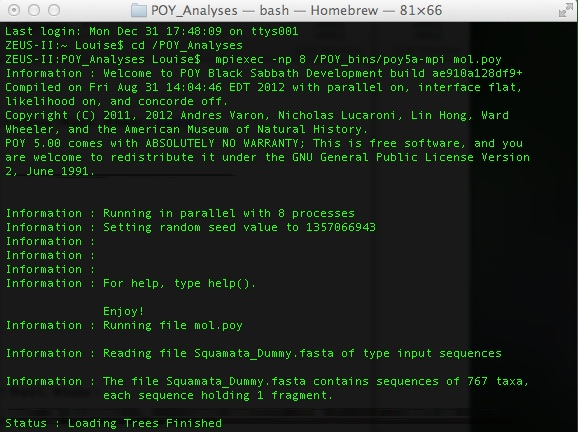
\includegraphics[width=0.9\textwidth]{doc/figures/mpiexec_script.jpg}
\end{center}
\caption{\poy flat interface displayed in a terminal window. The 
interface indicates that the program has been compiled with `parallel 
on'. The program is running the script \texttt{mol.poy} in parallel 
over 8 processors. In this case, MPICH is used to communicate 
processes during  parallel execution.}
\label{fig:mpiexecscript}
\end{figure}

%-----------------------------------
%The Graphical User Interface
%-----------------------------------

\section{The Graphical User Interface}

Two of the working environments that \poy provides are the
\emph{Graphical User Interface} and the \emph{Interactive Console}
(also known as the \emph{ncurses} interface). The \emph{Graphical
User Interface} has a user-friendly appearance like other native
stand-alone applications where different functions are accessible
through menus and windows. Thus, the entire analysis can be carried
out by clicking on appropriate selections and, where necessary,
typing specifications in designated fields. Currently, the
\emph{Graphical User Interface} is designed for the analysis of
data with parsimony or likelihood (with minimal model selection)
as the optimality criterion.  Unlike the \emph{Interactive Console},
it is not possible to specify all options with the \emph{Graphical
User Interface}.  The minimum screen size for the \emph{Graphical
User Interface} is 1024 x 768 pixels.

On the other hand, the \emph{Interactive Console} requires a detailed
knowledge of \poy commands, their arguments, and the conventions
of \poy scripting. All these features are described in the \emph{POY
Commands} chapter (\ref{commands}).

Even though the Mac OSX version of the \emph{Graphical User Interface}
is used for screen shots throughout this chapter, the Windows version
contains the same items and functionality, differing only in the
generic window format specific to the platform.

When \poy is first opened, two items appear on the screen: the \poy
menu bar across the top and the \emph{POY Launcher} window
(Figure~\ref{fig:menu_launcher_window}).

[Note: In Windows the menu bar is within the launcher window.]

\begin{figure}[htpb]
\begin{center}
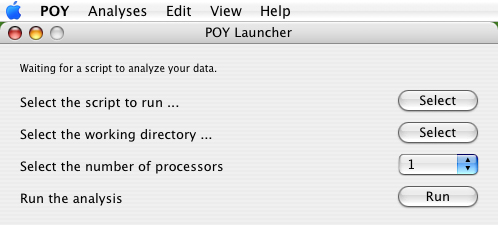
\includegraphics[width=0.75\textwidth]{doc/figures/menu_launcher_window.jpg}
\end{center}
\caption{The \poy menu bar and the \emph{POY Launcher} window. 
These items appear when \poy is opened.}
\label{fig:menu_launcher_window}
\end{figure}

\subsection{POY menu bar}
The menu bar contains the following drop-down menus:
\begin{description}
\item[POY] (Mac OSX only) Contains generic items as with other 
Mac OSX applications. This pull down menu allows selection of the 
\emph{About POY} window (Figure~\ref{fig:about_window}) that 
lists the current version of \poy, a copyright statement, and the address 
of the \poy website. In addition, it includes a \emph{Quit POY} tab 
that closes the program. 
\item[Analyses]    Contains options for different types of tree searches, 
calculation of support values, tree diagnosis, and their respective outputs. 
Other items in this menu open the \emph{POY Launcher} 
(Open Launcher) and the \emph{Interactive Console}.
\item[Edit] Contains standard tools for undoing, cutting, copying, 
pasting, deleting, and selecting.
\item[View] opens the \emph{Output} window to display the results 
(including warning and error messages) and the current state of the analysis. 
This \emph{Output} window also contains an \emph{update} tab.  
It also contains the \emph{About POY} menu item in Windows. %and Linux.  
\item[Help] Opens the \poy \emph{Manual} in PDF format (requires 
a PDF viewer).
\end{description}

\begin{figure}[htpb]
\begin{center}

\includegraphics[width=0.5\textwidth]{doc/figures/about_window.jpg}
\end{center}
\caption{The \emph{About POY} window.}
\label{fig:about_window}

\end{figure}

\subsection{POY Launcher} 
The \emph{POY Launcher} is the only window that automatically 
opens upon starting \poy. This allows the user to import a previously 
created script, designate a working directory, specify the number of 
processors, and start the analysis.

\begin{description}
\item[Select the script to run] 
Allows the user to specify the location of a \poy script.
\item[Select the working directory] 
The working directory is the directory that contains 
the input data and output files. By default, the working directory is set to 
be the same as the directory containing the selected \poy script. 
\item[Select the number of processors] 
If more than one processor or core is available, up to 
8 can be designated for running the analysis. It is important to note 
that once specified, the selection is applied to \emph{all} subsequent 
analyses in the current \poy session. Table \ref{ParallelizationGuide} 
is a guide to the parallelization ability of \poy depending on the operating 
system and the \poy interface being used. Observe that parallelization 
is \textbf{\emph {never}} supported in interactive sessions, see 
Section~\ref{interactiveconsole}.
\item[Run the analysis] 
Clicking the \emph{Run} button starts the execution of the selected 
script. Once the script is initiated, the \emph{Run} button becomes 
the \emph{Cancel} button that can be used to interrupt a \poy session.
\end{description}

\begin{table}[t] 
\small
\caption{Parallelization Guide. The field `mpi+' indicates that mpi 
must be enabled during compiling. A distinction is made between the 
\emph{Interactive Console} or \emph{ncurses} that is downloaded as 
binaries (\texttt{bins}) from the website and that which is compiled 
from the source (\texttt{src}).} 
\label{ParallelizationGuide} 
\begin{center}
\renewcommand{\arraystretch}{1.5}
\begin{tabular}{p{2.7cm}  p{1.1cm}  p{3.0cm}  p{3.0cm}  p{0.75cm}} 
\hline
Operating System & GUI & Interactive Console (bins) & Interactive Console (src) & Flat \\
\hline
Mac OSX & + & -- & -- & mpi+ \\
Windows & + & -- & -- & mpi+ \\
Linux & N/A & -- & -- & mpi+ \\
\hline
\end{tabular}
\end{center}
\end{table}

If the \emph{Run} button is clicked without the selected script and
working directory, or the names of the scripts and working directory 
are entered incorrectly, \poy issues an error message in the upper part 
of the \emph{POY Launcher} window, such as \texttt{POY finished 
with an error}.

\subsection{The \emph{Analyses} menu}
The \emph{Analyses} menu is the main toolbox of the \poy \emph{GUI} 
interface (Figure~\ref{fig:simple_search_window}, left). Selections are 
subdivided into four functional categories. The first three deal with tree 
searching, support calculation, and tree diagnosis; the fourth one is used 
for  script management or interactive command execution that bypasses the 
menu-driven script generation. Each of the menu items is described below 
in the order it appears on the menu.

Most options are consistently applied through different kinds of analysis. 
Therefore, all options are described in detail only for the \emph{Simple Search} 
analysis. The descriptions of other analyses are made with reference to the the 
\emph{Simple Search} and focus on unique options.

%-----------------------------------
%Tree search options
%-----------------------------------

\subsubsection{Tree searching options}

A number of different tree searching options are available through
the \emph{Graphical User Interface}.  These include a \emph{Simple
Search}, \emph{Timed Search}, \emph{Search with Ratchet} and
\emph{Search with Perturb}.

\subsubsection*{\emph{Simple Search}} 
The \emph{Simple Search}
window permits the analysis of a number of different data types,
including a range of molecular characters (from DNA sequences to
complete genomes), custom alphabet characters, and qualitative
characters, under parsimony.  It is also possible to carry out a
likelihood analysis of DNA sequence, morphological and qualitative
data under a number of different models.  In the simplest sense, a
typical search involves a series of steps.  First, initial trees
are generated by random addition sequence from the imported character
data.  These trees are then subjected to branch swapping, after
which trees are selected to report.  The \emph{Simple Search} window
(Figure~\ref{fig:simple_search_window}, right) provides the most
common and basic options for a standard tree search in \poy that
must be selected by either clicking the appropriate buttons or by
typing. Note that \emph{all} the empty fields must be filled in
(even if that means assigning a cost of \texttt{0} to all the
\emph{Sequence Parameters}), otherwise the default values will be
used. The window is subdivided into five sections: 

\begin{figure}
\centering
\begin{minipage}[c]{0.45\textwidth}
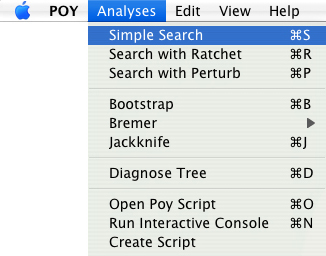
\includegraphics[width=\textwidth]{doc/figures/simplesearch_menu.jpg}
\end{minipage}
\,
\begin{minipage}[c]{0.52\textwidth}
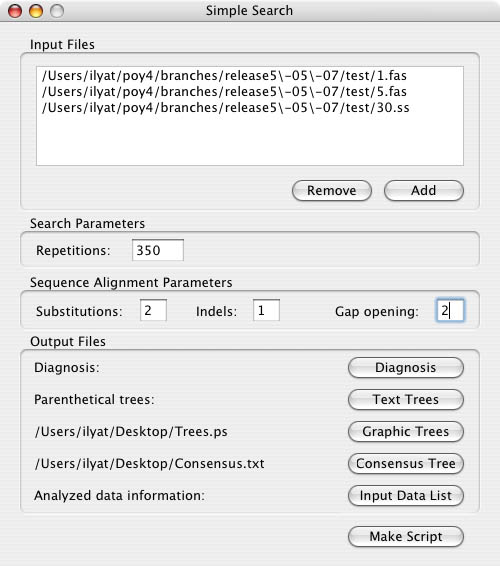
\includegraphics[width=\textwidth]{doc/figures/simplesearch_window_filled.jpg}
\end{minipage}

\caption{The \emph{Simple Search} window. Selecting \emph{Simple Search} 
from the \emph{Analysis} 
menu (left) opens the \emph{Simple Search} window options (right).}
\label{fig:simple_search_window}
\end{figure}

\begin{description}
\setlength{\parindent}{0.5cm}
\item[Input Files]
Contains the list of files that are to be input into \poy. These include
character files in nucleotide, Hennig86, and Nexus formats, as well 
as tree files. Continuous characters can be input into \poy in a Hennig86 
format matrix (see~\ccross{read}). Character data in other formats can 
be input by specifying additional arguments in the script (see~\ccross{read}).

\begin{statement}
Gap-opening cost greater than $0$ can not be specified with 
prealigned data as the columns are treated as independent in 
this file format.
\end{statement}

\item[Search Parameters]
Holds one field to set the number of independent random addition Wagner 
replicates to be generated.

\item[Input Parameters]
Holds fields to specify the optimality criterion (parsimony or likelihood).  
With \emph{Parsimony} as the optimality criterion, it is possible to select 
different datatypes (sequence, chromosome, genome, custom alphabet, 
break inversion or qualitative) and allows the user to select whether these data 
should be treated as prealigned (if possible). Selection of different datatypes 
will invoke an additional subsection (see below).  Currently, it is only possible 
to analysis sequence and qualitative data with the maximum likelihood criterion.
\end{description}   

\hangindent=1cm	\emph{Parsimony Optimality Criterion}
The parameters in this section are dependent on the data types selected 
in \emph{Input Parameters}. More detailed explanations of the different 
data types can be found below and  in the difference character types 
sections of both~\ccross{read} and ~\ccross{transform}.

\begin{description}
%\setlength{\labelwidth}{0pt}
\setlength{\labelsep}{5pt}
\setlength{\itemindent}{0pt}%
\setlength{\parindent}{0.5cm}        

\item [Sequence Parameters]  If \emph{sequence} data types are
chosen, the user can specify the substitution, indel, and gap opening
costs of sequences. Enter \texttt{0} if no gap opening cost is
desired. If the value of a parameter is not specified, default
values are used.  The default value for both substitutions and
insertion deletion events is \texttt{1} and that of gap-opening is
\texttt{0}.

\item [Chromosome and Mauve Parameters] \emph{Chromosome} characters
are multi-locus nucleotide sequences and can include nuclear
chromosomes, as well as, mitochondrial and viral genomes.  It is
possible to submit either \poyargument{annotated} (by selection of
the \emph{Annotated} box) or \emph{Unannotated} (by leaving the
\emph{Annotated} box unchecked) chromosomes. Within \emph{Annotated}
chromosomes, homologous regions, such as loci, are separated with
the pipe symbol (``$\vert$'').  \emph{Unannotated} chromosomes are
entirely without delimiters. For \emph{Unannotated} chromosomes,
the Mauve Parameters, must be set by the user.  These parameters
(\emph{Match Quality, Match Coverage, Min. Match} and \emph {Max.
Match}) are employed by the Mauve aligner to find regions of homology
or synteny blocks between chromosomes (see~\nccross{annotate}{annotate}
within the command \poycommand{transform}). Default values for these
parameters are provided in the \emph{GUI}.

\indent Within this subsection it is necessary to specify both
\emph{Locus Indel} and rearrangement (\emph{Locus Breakpoint} or
\emph{Locus Inversion}) costs.  The cost of a \emph{Locus Indel}
is by default set to 10 plus 0.9 times the length of the locus
(see~\nccross{locus\_indel} {chromosomelocusindel}  within the
command \poycommand{transform}).  Rearrangements of homologous
regions---as defined by the user in the case of \emph{Annotated}
chromosomes or as determined by the Mauve aligner as in \emph{Unannotated}
chromosomes)---are then optimized using either \emph{Locus Breakpoint}
or \emph{Locus Inversion} costs
(see~\nccross{locus\_breakpoint}{chromosomelocusbreakpoint} and
~\nccross{locus\_inversion}{chromosomelocusinversion} within the
command \poycommand{transform}).  The default cost for both is set
to 10. The user must also specify the \emph{Median solver} for the
optimization of rearrangements of \emph{Annotated} chromosomes.
The default median solver is \emph{Caprara}, but the user can
alternatively choose \emph{BBTSP, ChainedLK, COALESTSP, MGR,
Siepel, SimpleLK} and \emph{Vinh}
(see~\nccross{median\_solver}{chromosomemediansolver} within the
command \poycommand{transform}).

\indent The user must also specify whether the chromosome is
\emph{Circular} (true) or linear (false).  It is not possible to
submit pre-aligned data files for either \emph{Annotated} or
\emph{Unannotated} chromosomes.


\begin{statement}
\textbf{Locus definition}. In the \emph{Sequence Parameters} section
for a parsimony analysis, the user may be required to specify the
cost associated with a \emph{Locus Breakpoint}, \emph{Locus Inversion}
or \emph{Locus Indel}, depending on the data type. In these cases,
\emph{Locus} should \textbf{not} be taken to be the functional,
biological unit in the classical sense, but only as a homologous
segment of a sequence.  \end{statement}

\item [Genome and Mauve Parameters] \emph{Genome} characters are
multi- \\locus, multi-chromosomal nucleotide sequences, wherein
transformations (i.e. indels, substitutions, and rearrangements)
are optimized at the sequence, locus \emph{and} chromosomal level.
Within the genome data file, individual chromosomes are separated
by the at symbol (``$@$'') and the individual chromosomes remain
\emph{Unannotated}.

\indent As with \emph{Unannotated Chromosome} characters, homologous
regions are determined using the Mauve parameters (\emph{Match
Quality, Match Coverage, Min. Match} and \emph {Max. Match}).
Default values for these parameters are provided in the \emph{GUI}.
The \emph{Locus Indel} and rearrangement (\emph{Locus Breakpoint}
or \emph{Locus Inversion}) costs are set by the user. By default,
the cost of a \emph{Locus Indel} is  set to 10 plus 0.9 times the
length of the locus (see the argument~\nccross{locus\_indel}
{chromosomelocusindel} within the \emph{Chromosome and genome
transformation methods} of the command \poycommand{transform}).
Rearrangements of homologous regions, as determined by the Mauve
aligner, are then optimized using either \emph{Locus Breakpoint}
or \emph{Locus Inversion} costs  (see the
arguments~\nccross{locus\_breakpoint}{chromosomelocusbreakpoint}
and~\nccross{locus\_inversion}{chromosomelocusinversion} within the
\emph{Chromosome and genome transformation methods} of the command
\poycommand{transform}).  The default cost for both is set to 10.
A \emph{Median solver} must also be specified for the optimization
of rearrangements: \emph{BBTSP, ChainedLK, COALESTSP, MGR, Siepel,
SimpleLK} and \emph{Vinh} (see the argument~\nccross{median\_solver}
{chromosomemediansolver} within the \emph{Chromosome and genome
transformation methods} of the command \poycommand{transform}).

\indent Two other costs must be set for the analysis of this data
type--\emph{Translocation} events and \emph{Chromosome Indel}. The
cost of the \emph{Translocation} of a region of one chromosome to
another chromosome is set to 10 by default.  The cost of the insertion
or deletion of an entire chromosome is by default set to 10 plus
0.9 times the length of the chromosome.

As with \emph{Chromosome} characters, it is not possible to input 
pre-aligned data files. 

\item [Custom Alphabet Parameters] \emph{Custom Alphabet} characters
are \\those that employ a user-specified alphabet. With this data
type, only insertion-deletion and substitution events are allowed.
\emph{Custom Alphabet} characters can be input as prealigned.  Within
this subsection, the user must specify the heuristic \emph{Level}
of the median sequence calculation. \emph{Direct Optimization} is
employed in median sequence calculation. Because calculating the
median states between custom alphabet strings becomes more
computationally intensive (and time consuming) as the number of
elements in the alphabet increases, the user should select a heuristic
level of median calculation appropriate for their data.  The default
level is 2.

\indent In addition to the data file, the user is require to upload
a \emph {Cost Matrix} that specifies the substitution and indel
transformation costs for alphabet elements.  By selecting the \emph
{Cost Matrix} button within this subsection, the user can upload a
cost matrix that specifies these costs for their custom alphabet
data. For details on the format requirements for custom alphabet
data files and their associated cost matrices see the
argument~\nccross{custom\_alphabet}{customalphabet} within the
command  \poycommand{read}.

\item [Break Inversion Parameters] \emph{Break Inversion} characters
are an enhancement of \emph{Custom Alphabet} characters. In addition
to allowing substitution and insertion deletion events, element
rearrangements, as well as orientation information can also be
optimized.  The median solvers provided restrict the analysis of
prealigned data.  The rearrangement costs for \emph{Break Inversion}
characters can be optimized using either \emph{Breakpoint} or
\emph{Locus Inversion} approaches (see the
arguments~\nccross{locus\_breakpoint}{chromosomelocusbreakpoint}
and~\nccross{locus\_inversion} {chromosomelocusinversion} within
the \emph{Chromosome and genome transformation methods} of the
command \poycommand{transform}). The default cost for both is set
to 10. A \emph{Median solver} must also be specified for the
optimization of rearrangements. The default median solver is
\emph{Caprara} \cite{Caprara2001}, but the user can alternatively
choose \emph{BBTSP, ChainedLK, COALESTSP, MGR}
\cite{bourqueandpevzner2002}, \emph{Siepel} \cite{siepelmoret2001},
\emph{SimpleLK} and \emph{Vinh} (the TSP solvers BBTSP, CoalesTSP,
ChainedLK and SimpleLK taken from the Concorde package)
(see~\nccross{median\_solver} {chromosomemediansolver}  within the
command \poycommand{transform}).  The calculation of median states
between \emph {Break Inversion} strings becomes more computationally
intensive (and time consuming) as the number of elements in the
alphabet increases, therefore a single heuristic level of median
calculation can only be employed for these character types--the
default level is 1.

\indent The requirements for \emph{Break Inversion} character types
are identical to those for \emph{Custom Alphabet} characters, with
respect to substitution and indel transformation costs.  By selecting
the  \emph{Cost Matrix} button within this subsection, the user can
upload a cost matrix to specify these costs. The user should see
the argument~\nccross{custom\_alphabet} {customalphabet} within the
command \poycommand{read} for details on the format requirements
for these cost matrices, which are identical in form to those for
\emph{Custom Alphabet} characters.

\item [Qualitative Parameters] \emph{Qualitative} data are any
non-sequence, prealigned data type (e.g. morphology, behavior).
These character types are optimized as additive, non-additive or
Sankoff characters and this information must be included in the
data file when using the \emph{Graphical User Interface}.

\end{description}

\hangindent=1cm  \emph{Likelihood Optimality Criterion} Currently,
it is only possible to perform a likelihood analysis of DNA sequences
(prealigned being permitted), %morphology and qualitative character
types. Using the \emph{GUI}, these data can be analyzed with
\texttt{likelihood} only (currently, transformation of the data to
\texttt{elikelihood} cannot be performed using the \emph{GUI}).
More detailed explanations of these options can be found below and
in the \emph{Likelihood transformation methods} section of
~\ccross{transform}.  In this section the user can specify the
\emph{likelihood model} of character substitution under which the
analysis will be performed.  Available substitution models include
JC69/Neyman, F81, K2P/K80, F84, HKY85, TN93, GTR, and NCM.  Users
can also perform phylogenetic model selection using AIC, AICc and
BIC.  Within this section it is possible to specify the nature of
among-site variation under \emph{Rate Distribution}.  Rate variation
distributions allow multipliers to be applied to separate groups
of characters.  These distributions can be set to \emph{Constant},
\emph{Gamma} (for non-zero rate variation) or  \emph{Theta} (for
parameterization of invariant sites).  These distribution values
can be specified for all of the available models. In addition,
\emph{Rate Classes} enables the user to specify the number of rate
classes for the discrete \emph{Gamma} rate distribution.  The user
can choose up to 8 rate classes for either \emph{Gamma} or \emph{Theta}
models (the default is 4).  \emph{Gap Treatment}  specifies the
treatment of indels.  There are three options \emph{missing},
\emph{character}, and \emph{character plus coupled}.  When gaps are
treated as \emph{missing}, they play no role in the calculation of
tree likelihoods.  The \emph{character} option treats the insertion
and deletion of A, C, G, and T each as different types of events
that are independently estimated (hence additional parameters over
\emph{coupled}). When \emph{coupled} is specified, all indel events
are treated with the same rate parameter.  \emph{Cost} specifies
the form of likelihood employed.  The options for prealigned data
(sequence and qualitative) are \emph{MAL} for \emph{maximum average
likelihood} and {MPL} for \emph{most parsimonious likelihood}
\cite{barryandhartigan1987}. Unaligned sequences can be optimized
with both \emph{MAL} (by transforming the sequences to
\poyargument{fixed\_states} first) and \emph{MPL}.  The prior
probabilities of the states are determined using \emph{Priors}.
The options are \emph{equal}, where each state prior is set to 1
divided by the number of states, and \emph{estimated}, where the
priors are set by their frequency in the data set.  Priors for gaps
are estimated by the maximum difference in length between input
sequences.

\begin{description}
\setlength{\parindent}{0.5cm}	   
\item[Output Files]
Designates the names and locations of files containing results of
the analysis.  By default, all of these output options are generated
with default names applied.  The names can then be changed in the
generated script or the option can be removed entirely.  As implied
by their respective titles, the \emph{tree} buttons output trees
in both parenthetical (best and consensus trees) and postscript
form (although this button only outputs a PDF file of the optimal
trees found, a useful commands that the user can include in the
generated script is to output a PDF file of the consensus tree (see
the argument~\nccross{graphconsensus}{graphconsensus} within the
command \poycommand{report})).

\indent A \emph{diagnosis} file provides information relating to
the analysis. Information in this file includes the cost of the
tree, the rearrangement costs (in the case of the analysis of
chromosome, genome and break inversion data types), as well as
information about each resulting node in the tree.  At each node,
the user is provided with a cost of the tree down to that node, a
rearrangement cost (if applicable), the ``descendant nodes'' coming
from this node and information concerning individual characters at
these nodes.

\begin{statement} The \texttt{root} in the diagnosis file may not
be the same as the root \poyargument{set} by the user.  This is
because the tree length heuristics may be based on an alternate
rooting scheme than that used for the \poyargument{newick} or
\poyargument {graphic trees} output.  \end{statement}

\indent The \emph{Analyzed data information} outputs a summary of
the input data. Specifically, the number of terminals to be analyzed,
a list of included terminals with numerical identifications, list
of synonyms (if specified), a list of excluded terminals, the number
of included characters in each character-type category (additive,
non-additive, Sankoff and sequence) with the corresponding cost
regimes, a list of excluded characters, and a list of input files.

\indent The \emph{Outgroup} field allows the the user to specify
the outgroup taxon.  The name of the taxon should reflect the name
as interpreted by \poy.  Therefore, the name should take into account
synonymy files, and taxon names that contain commented out information
via use of a \$ sign (see the argument~\nccross{rename}{rename}).
\end{description}

\begin{figure}
\centering
\begin{minipage}[c]{0.45\textwidth}
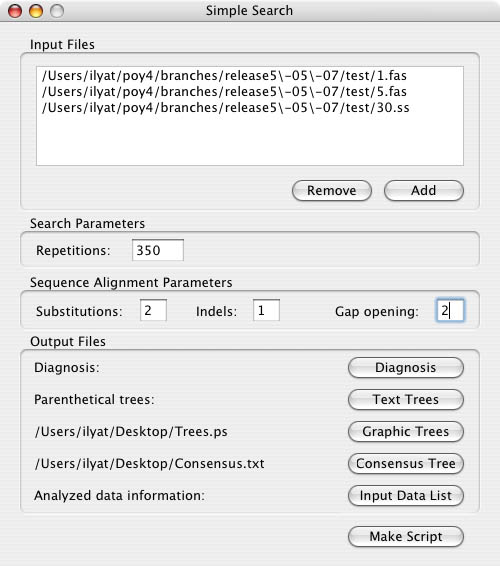
\includegraphics[width=\textwidth]{doc/figures/simplesearch_window_filled.jpg}
\end{minipage}
\,
\begin{minipage}[c]{0.52\textwidth}
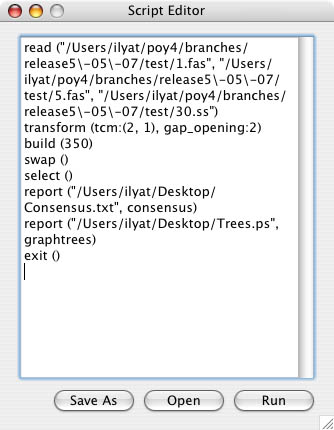
\includegraphics[width=\textwidth]{doc/figures/simplesearch_script.jpg}
\end{minipage}

\caption{The \emph{Simple Search} window with specified search 
parameters (left) and the corresponding \emph{Script Editor} window. 
Observe that the names of the output files are left as the default output names.}
\label{fig:ScriptEditor_Window}
\end{figure}

Once all the parameters are selected, click the \emph{Make Script} button 
and another window--the \emph{Script Editor}--containing the generated 
script, appears on screen (Figure~\ref{fig:ScriptEditor_Window}). 
The script can be edited by typing in the commands directly in the 
\emph{Script Editor} window, saved (by clicking the \emph{Save As} 
button), or replaced with another script (using the \emph{Open} button). 
To start the analysis, click the \emph{Run} button in the \emph{Script 
Editor} window. When the \emph{Run} button is clicked, \poy will issue a
request to save the script. Thus, not only does \poy execute the script but
it also creates the record of the type of analysis (including all user-defined 
specifications) that was performed. Moreover, these scripts can later be 
executed manually in the \emph{ncurses} or \emph{flat} interfaces, or
selected as a script to run in the \emph{Graphical User Interface}.

\subsubsection*{\emph{Timed Search}}

{\emph{Timed Search} (Figure~\ref{fig:timed_search}) implements a
default search strategy that effectively combines tree building
with TBR branch swapping, parsimony ratchet, and tree fusing.  The
\emph{Timed Search} window has the same four parameter groups
described for the \emph{Simple Search}. However, the \emph{Search
Parameters} section (called \emph{Search and Perturb Parameters})
contains four fields specifying the search targets instead of the
\emph{Repetitions} field. These include the following:


\begin{figure}
\centering
\begin{minipage}[c]{0.45\textwidth}
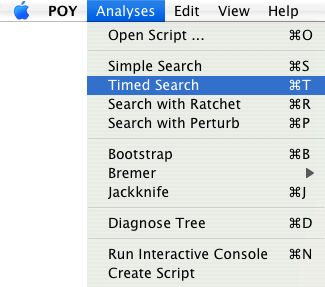
\includegraphics[width=\textwidth]{doc/figures/timedsearch_menu.jpg}
\end{minipage}
\,
\begin{minipage}[c]{0.52\textwidth}
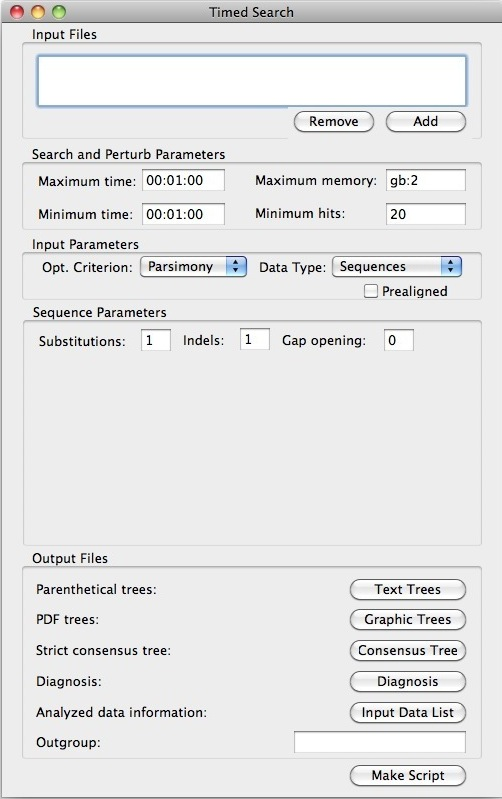
\includegraphics[width=\textwidth]{doc/figures/timedsearch_window.jpg}
\end{minipage}

\caption{The \emph{Timed Search} window. Selecting \emph{Timed Search} 
from the \emph{Analysis} menu (left) and viewing the \emph{Timed Search} 
window options (right).}
\label{fig:timed_search}
\end{figure}

\begin{description}
\item[Maximum time] The maximum total execution time for the search. 
The time is specified as days:hours:minutes.
\item[Minimum time] The minimum total execution time for the search. 
The time is specified as days:hours:minutes.
\item[Maximum memory] The maximum amount of memory allocated 
for the search.
\item[Minimum hits] The minimum number of times that the minimum 
cost must be reached before terminating the search.
\end{description}

This heuristic search is a powerful tool for analyzing data. The
number of rounds of successive searching is limited only by the
previously specified search targets. Therefore, when performing a
\emph{Timed Search}, it is {\bf crucial} to set the maximum time
such that the program has a reasonable amount of time to perform a
search.  Thus, it is important to have some approximation as to the
length of time it would take to perform a single round of searching
(e.g. build (1), followed by TBR, ratchet and fusing in the case
of a parsimony analysis of DNA sequence data).  Clearly, this is
data and optimality criterion dependent.  With this information,
the user can then estimate the amount of time necessary to perform
a thorough search (perhaps 10 times the amount of time it took to
perform this single round of build, swap, ratchet and fusing).  The
user should also allow some time for the program to collate and
write the results to files.  If the user has opted to run this
analysis in parallel, this can take some time.

\subsubsection*{\emph{Search with Ratchet}}

The parsimony ratchet is a heuristic strategy to escape  local
optima during tree searching~\cite{Nixon1999}. The ratchet reweights
a given percentage of characters for a specified number of iterations
of a search. An analysis is then performed and the resulting tree
topology is evaluated using the original data matrix with all
characters (with original weights) to determine the length of the
tree. The \emph{Search with Ratchet}
(Figure~\ref{fig:search_with_ratchet_window}) follows the same basic
steps of a simple search but includes the ratchet step after the
swap. In addition to the same sequence alignment and search parameters
as described for the \emph{Simple Search} window, the \emph{Search
Parameters} section provides the following ratchet parameters fields:


\begin{description}
\item[Ratchet iterations] The number of iterations for the parsimony
ratchet.
\item[Severity] The severity parameter of the ratchet (the weight
change factor for the selected characters).
\item[Percentage] The percentage of characters to be reweighted during 
ratcheting.
\end{description}

\begin{figure}
\centering
\begin{minipage}[c]{0.45\textwidth}
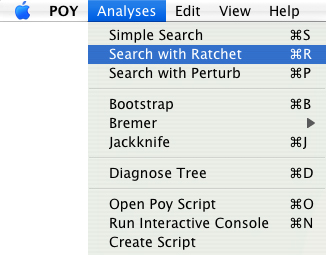
\includegraphics[width=\textwidth]{doc/figures/searchwithratchet_menu.jpg}
\end{minipage}
\,
\begin{minipage}[c]{0.52\textwidth}
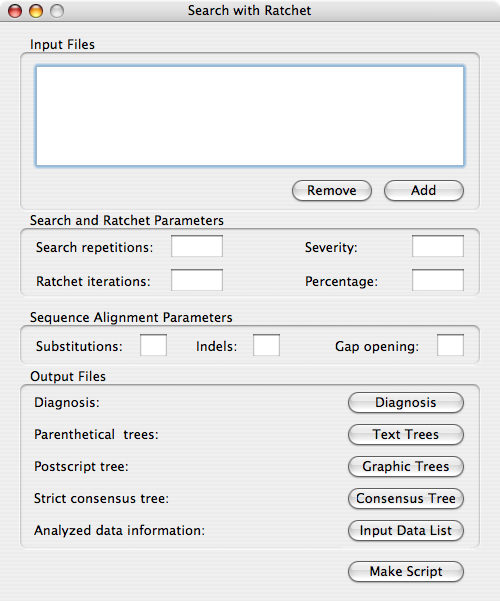
\includegraphics[width=\textwidth]{doc/figures/searchwithratchet_window.jpg}
\end{minipage}

\caption{The \emph{Search with Ratchet} window. Selecting \emph{Search 
with Ratchet} from the \emph{Analysis}  menu (left) and viewing the 
\emph{Search with Ratchet} window options (right).}
\label{fig:search_with_ratchet_window}
\end{figure}

\subsubsection*{\emph{Search with Perturb}}

\emph{Search with Perturb} (Figure~\ref{fig:search_with_perturb_window})
provides an alternative means to escape local optima by changing
the transformation cost matrix of the sequence characters, a procedure
similar in spirit to the parsimony ratchet. In addition to the same
sequence optimization and search parameters as described for the
\emph{Simple Search} window, the \emph{Search with Perturb} window
provides three extra fields with the parameters for the transformation
cost matrix perturbation as follows:

\begin{figure}
\centering
\begin{minipage}[c]{0.45\textwidth}
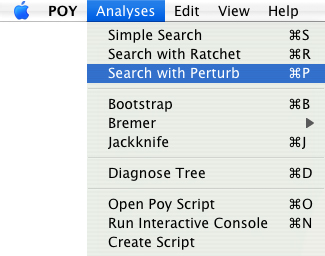
\includegraphics[width=\textwidth]{doc/figures/searchwithperturb_menu.jpg}
\end{minipage}
\,
\begin{minipage}[c]{0.52\textwidth}
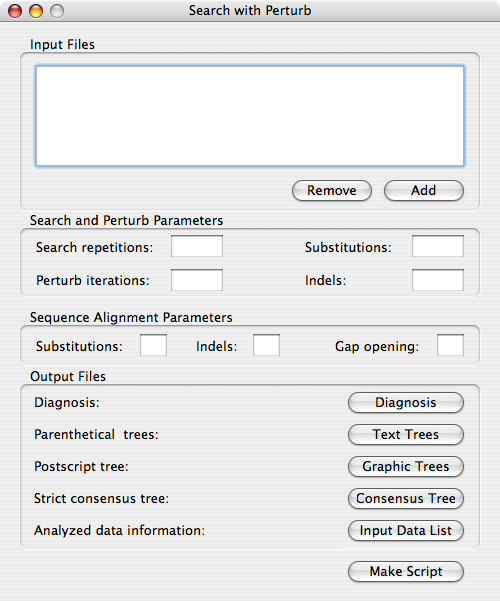
\includegraphics[width=\textwidth]{doc/figures/searchwithperturb_window.jpg}
\end{minipage} 
\caption{The \emph{Search with Perturb} window. Selecting \emph{Search with 
Perturb} from the \emph{Analysis} menu (left) and viewing the \emph{Search 
with Perturb} window options (right).}
\label{fig:search_with_perturb_window}
\end{figure}

\begin{description}
%\setlength{\labelwidth}{0pt}
%\setlength{\labelsep}{5pt}
%\setlength{\itemindent}{0pt}%
\item[Perturb iterations] Sets the number of perturb iterations to be performed.
\item[Substitutions] Specifies the cost of the perturbed substitutions.
\item[Indels] Specifies the cost of the perturbed indels.
\end{description}

During this heuristic search, \poy performs a parsimony ratchet search during 
each iteration (default values are used, i.e. 25\% probability, 2 severity).

\subsubsection{Support calculation options}

It is possible to calculate several support values using this
interface.  Two of these measures, Bootstrap and Jackknife, involve
resampling techniques, while the third, Bremer support, is an
optimality-based measure based on the cost of the tree.

Although it is possible to calculate Jackknife and Bootstrap support
values for trees constructed using dynamic homology characters, it
is recommended against doing so as resampling of dynamic characters
occurs at the fragment, rather than nucleotide, level. Consequently,
the bootstrap and jackknife support values calculated for dynamic
characters are not directly comparable to those calculated based
on static character matrices. If it is desired to perform character
sampling at the level of individual nucleotides, the dynamic
characters must be transformed into static characters using
\poyargument{static\_approx} argument of the command~\ccross{transform}
prior to executing \poycommand{calculate\_support}.  Of course, if
the dataset of dynamic characters contains a large number of
fragments, this caveat may not be warranted.

For chromosome and genome character types, only the calculation of
Bremer support values is recommended.

None of the support calculation windows include functions for tree
building and searching. Therefore, one of the input files must
contain trees for which support values are going to be calculated.

\subsubsection*{\emph{Bootstrap}}

As a resampling technique, the non-parametric \emph{Bootstrap}
resamples the original data (with replacement), creating a simulated
dataset equal to the size of the original dataset. The \emph{Bootstrap}
window (Figure~\ref{fig:bootstrap}) specifies parameters for
estimating the Bootstrap support values. In addition to the
\emph{Simple Search} window fields, it contains a field for the
bootstrap parameters, in this case a \emph{Pseudoreplicates} field,
to specify the number of bootstrap pseudoreplicates.

\begin{description}
\item[Pseudoreplicates] Specifies the number of resampling iterations.
\end{description}

\begin{figure}
\centering
\begin{minipage}[c]{0.45\textwidth}
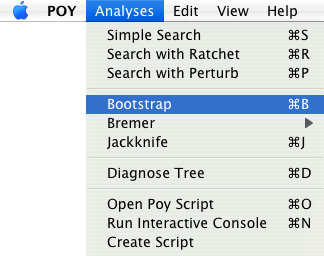
\includegraphics[width=\textwidth]{doc/figures/bootstrap_menu.jpg}
\end{minipage}
\,
\begin{minipage}[c]{0.52\textwidth}
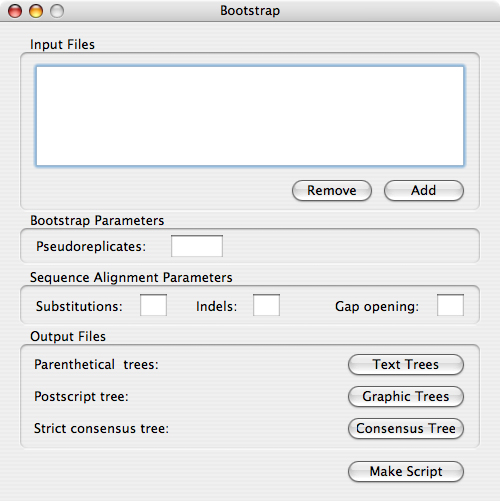
\includegraphics[width=\textwidth]{doc/figures/bootstrap_window.jpg}
\end{minipage}
\caption{The \emph{Bootstrap} window. Selecting \emph{Bootstrap} 
from the \emph{Analysis} menu (left) and viewing the \emph{Bootstrap} 
window options (right).}
\label{fig:bootstrap}
\end{figure}

\subsubsection*{\emph{Jackknife}}

An alternative statistical measure of support is the \emph{Jackknife}, 
wherein the original data matrix is resampled, but in this case without 
replacement.  The \emph{Jackknife} window (Figure~\ref{fig:jackknife}) 
specifies parameters for estimating the Jackknife support values. In 
addition to the \emph{Simple Search} window fields, \emph{Jackknife 
Parameters} contains fields to specify the number of Jackknife 
pseudoreplicates (\emph{Pseudoreplicates}) and the number of characters 
to be removed (\emph{Remove}) during each pseudoreplicate.

\begin{figure}
\centering
\begin{minipage}[c]{0.45\textwidth}
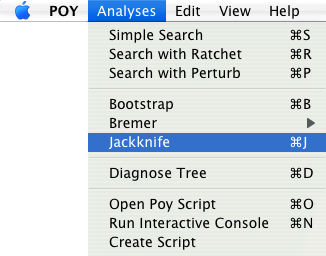
\includegraphics[width=\textwidth]{doc/figures/jackknife_menu.jpg}
\end{minipage}
\,
\begin{minipage}[c]{0.52\textwidth}
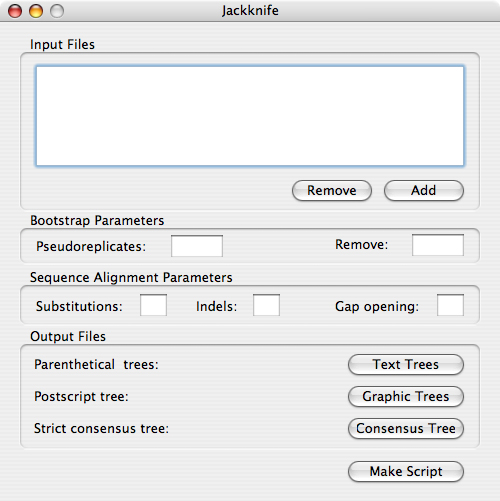
\includegraphics[width=\textwidth]{doc/figures/jackknife_window.jpg}
\end{minipage}
\caption{The \emph{Jackknife} window. Selecting \emph{Jackknife} 
from the \emph{Analysis} menu (left) and 
viewing the \emph{Jackknife} window options (right).}
\label{fig:jackknife}
\end{figure}

\begin{description}
\item[Pseudoreplicates] Specifies the number of resampling iterations.
\item[Remove] Specifies the percentage of characters being deleted 
during a pseudoreplicate.
\end{description}

\subsubsection*{\emph{Bremer}}

As an optimality-based measure of calculating tree support, Bremer
values are the number of extra steps required before a clade is
lost in the most parsimonious or strict consensus of the most
parsimonious trees.  Bremer support under likelihood is equivalent
to the log of the likelihood ratios for each branch~\cite{Wheeler2006}.
There are two ways to determine Bremer support values in \poy.  The
first involves performing a series of searches, where each group
supported on the examined cladogram is constrained not to occur in
the result.  The second does not involve constraining the tree but
collects information for all the clades not present in the set
visited trees.  Currently, calculating support via ``visited'' trees
can only be performed sequentially and not parallel.

The \emph{Bremer} option (Figure~\ref{fig:search_for_bremer_menu})
is divided into two windows: the \emph{Search for Bremer} window,
that specifies the Bremer support \cite{Bremer1988, Kallersjoetal1992}
calculation parameters, and the \emph{Report Bremer} window to
format the output of the results (Figure~\ref{fig:search_report_bremer}).

\paragraph{Search for Bremer}

\begin{figure}[htpb]
\begin{center}
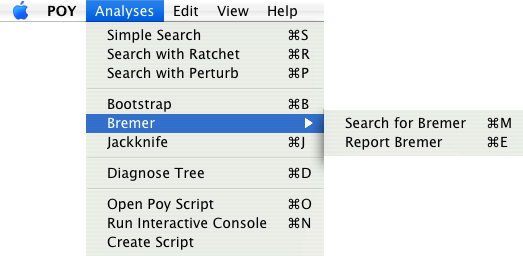
\includegraphics[width=0.65\textwidth]{doc/figures/searchforbremer_menu.jpg}
\end{center}
\caption{ Selecting the \emph{Bremer} windows from the \emph{Analysis} menu.}
\label{fig:search_for_bremer_menu}
\end{figure}

\begin{figure}
\centering
\begin{minipage}[c]{0.45\textwidth}
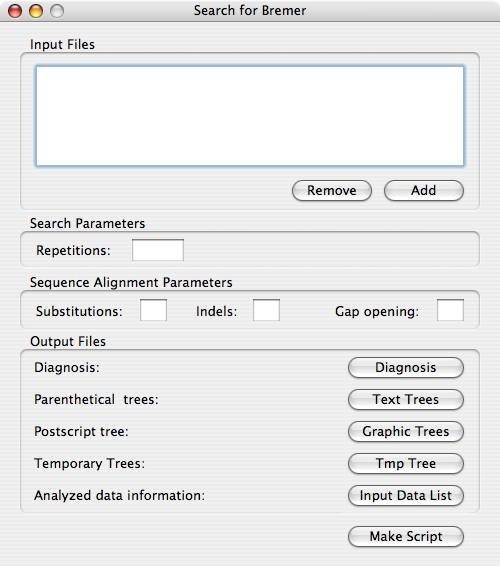
\includegraphics[width=\textwidth]{doc/figures/searchforbremer_window.jpg}
\end{minipage}
\,
\begin{minipage}[c]{0.52\textwidth}
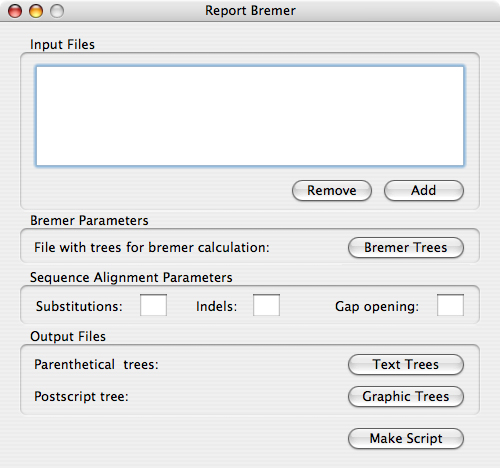
\includegraphics[width=\textwidth]{doc/figures/reportbremer_window.jpg}
\end{minipage}
\caption{Viewing the options of the \emph{Search for Bremer} (left) and the 
\emph{Report Bremer}(right) windows.}
\label{fig:search_report_bremer}
\end{figure}

The script produced in this window collects trees visited during a search for 
Bremer support calculations. This search can take a long time, as the goal of 
this search strategy is to broadly sample variation among trees, and guarantee 
that all clades have Bremer support values.  

In addition to the standard four sections defined for the \emph{Simple Search} 
window, that one of the output files is the \emph{Temporary Trees} file, which 
contains all the information required to produce the Bremer support tree
results in the \emph{Report Bremer} window. Make sure to choose a file 
name that does not overwrite this output.

If the search does not finish within the time frame available to the user the search 
can be interrupted and the intermediate results remain stored in the \emph{Temporary 
Trees} file.  As Bremer calculations are upper-bound values, terminating the search 
prior to completion and, thus, storing a smaller pool of visited trees may inflate 
support values relative to those generated by a more exhaustive search. The trees 
from the \emph{Temporary Trees} file can then be reported using the 
\emph{Report Bremer} window.

\paragraph{Report Bremer}
The script produced in this window takes the \emph{Temporary Trees} file 
generated in the \emph{Search for Bremer} window in the \emph{File with 
trees for Bremer calculation} field. 

\subsubsection{Diagnosis}
\subsubsection*{\emph{Diagnose Tree}}

The \emph{Diagnose Tree} window (Figure~\ref{fig:diagnosetree}) specifies 
parameters for reporting a diagnosis of the input tree. This window lacks the 
\emph{Search Parameters} section because the diagnosis is performed on 
the trees resulted from prior searches and no new trees are generated during 
the diagnosis procedure. In addition to the tree (or trees) file, the user must have 
input the data file associated with this tree file, in order to diagnose
the tree(s) in this file.

\begin{figure}[ht]
\centering
\begin{minipage}[c]{0.45\textwidth}
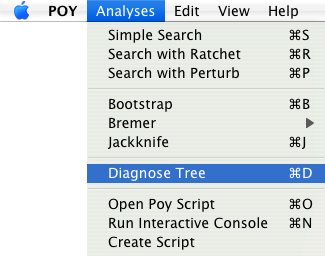
\includegraphics[width=\textwidth]{doc/figures/diagnose_menu.jpg}
\end{minipage}
\,
\begin{minipage}[c]{0.52\textwidth}
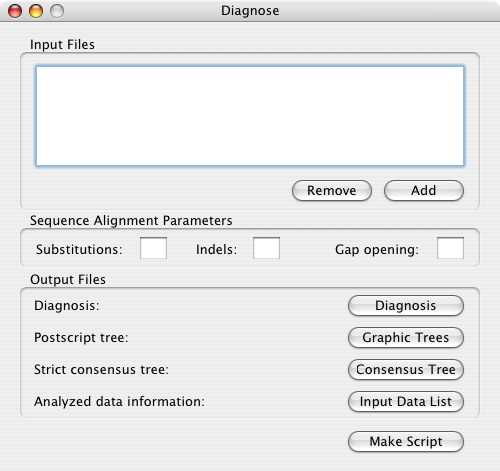
\includegraphics[width=\textwidth]{doc/figures/diagnose_window.jpg}
\end{minipage}
\caption{The \emph{Diagnose} window. Selecting \emph{Diagnose Tree} 
from the \emph{Analysis} menu (left) and viewing the \emph{Diagnose} 
window options (right).}
\label{fig:diagnosetree}
\end{figure}

\subsubsection{\emph{Script editing and the Interactive Console}}

\subsubsection*{Open POY Launcher}

Selecting \emph{Open POY Script} (Figure~\ref{fig:open_poy_launcher}) 
displays the \emph{POY Launcher} window (Figure~\ref{fig:menu_launcher_window}), 
the function of which is described above.

\begin{figure}[htpb]
\begin{center}
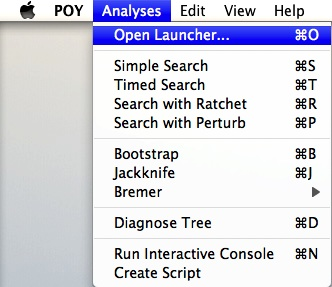
\includegraphics[width=0.5\textwidth]{doc/figures/openpoylauncher_menu.jpg}
\end{center}
\caption{The \emph{Open POY Launcher} selection opens the \emph{POY 
Launcher} window.}
\label{fig:open_poy_launcher}
\end{figure}

\subsubsection*{Run Interactive Console}

Selecting \emph{Run Interactive Console} (Figure~\ref{fig:runinteractive}) 
opens the \emph{ncurses} interface that enables the user to run the analysis 
interactively by entering \poy commands directly via the command-line 
interface of the \emph{Interactive Console} See \emph{Using the 
Interactive Console} (Section \ref{interactiveconsole}).

\begin{figure}
\centering
\begin{minipage}[c]{0.45\textwidth}
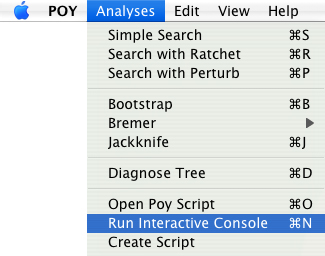
\includegraphics[width=\textwidth]{doc/figures/runinteractive_menu.jpg}
\end{minipage}
\,
\begin{minipage}[c]{0.52\textwidth}
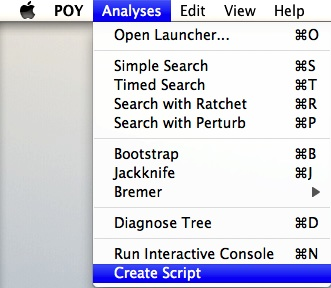
\includegraphics[width=\textwidth]{doc/figures/create_script_menu.jpg}
\end{minipage}
\caption{The \emph{Run Interactive Console} selection (left) opens \poy 
interactive console in a new window. The \emph{Create Script} selection 
opens the \emph{Script Editor} window (Figure~\ref{fig:ScriptEditor_Window}).}
\label{fig:runinteractive}
\end{figure}

\subsubsection*{Create Script}
The \emph{Create Script} selection opens a blank \emph{Script Editor} 
window that allows opening, creating, modifying, saving, and executing  
a customized script.

\subsection{The \emph{View} menu}

The \emph{View} menu contains the \emph{Output} window which is 
subdivided into two fields: the upper \emph{Results and Errors} and lower 
\emph{Status of Search} (Figure~\ref{fig:results_and_status_windows}). 
These fields display, respectively, the results (including warning and error 
messages) and the current state of the analysis. These fields are not updated 
automatically and in order to display the current state of the analysis the 
user must click the \emph{Update} button. The \emph{View} menu also 
contains the \emph{About POY} window in Windows.

\begin{figure}
\centering
\begin{minipage}[c]{0.45\textwidth}

\includegraphics[width=\textwidth]{doc/figures/view_menu.jpg}
\end{minipage}
\,
\begin{minipage}[c]{0.52\textwidth}
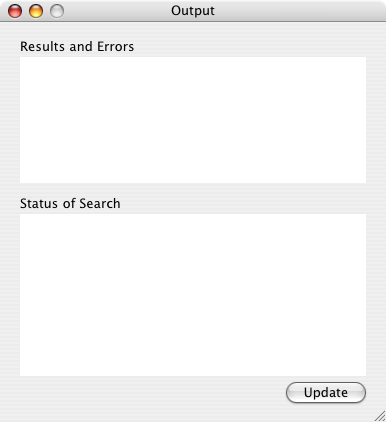
\includegraphics[width=\textwidth]{doc/figures/output_window.jpg}
\end{minipage}
\caption{Selecting the \emph{Output} window (left) and viewing the 
\emph{Results and Errors} and  \emph{Status of Search} fields.}
\label{fig:results_and_status_windows}
\end{figure}

%-----------------------------------
%Interactive Console
%-----------------------------------
\section{Using the Interactive Console} \label{interactiveconsole}

This section will help you get started using the \poy \emph{Interactive 
Console} and will prepare you for the more extensive, technical descriptions 
in the next chapter, \emph{\poy Commands}.
This section will illustrate how to input data files, check the data you are 
analyzing, generate a set of initial trees, do basic branch 
swapping to find a local optimum, and, finally, produce and visualize 
the resultant trees, their consensus, and generate support 
values in a command-line environment rather than using a 
\emph{Graphical User Interface}. 

For the purpose of this exercise, two data files, which are included in the 
download package, are available at the \poy download page.\\
\begin{center}
\url{http://www.amnh.org/our-research/computational-sciences/research/projects/systematic-biology/poy/download}
\end{center}

\begin{itemize}
\item {\texttt{28s.fas} contains unaligned DNA sequences (partial 28S 
ribosomal RNA) in FASTA format.~\cite{pearson1988}}
\item {\texttt{morpho.ss} contains a morphological data matrix in 
Hennig86 format.~\cite{farris1988}}
\end{itemize}

Once \poy has been launched and the interface (Figure~\ref{fig:figinterface})  
appears on the screen, data can be input and analysis can proceed. As you 
follow the instructions, you are encouraged to consult the help file by using 
the command \commandstyle{help} (see Section~\ref{sec:help} to learn 
more about \poy commands and their arguments).

\subsection{The interface}

The \emph{Interactive Console} provides a terminal environment with
enhanced ability to display the results and the state of the analysis.
We recommend the use of the console to explore and verify the data
in the early steps of the analysis, and to learn the scripting
language. Using the console requires familiarity with \poy commands,
their arguments, and the conventions of \poy scripting (which are
discussed in the \emph{POY Commands} chapter). It has four windows:
\emph{POY Output}, \emph{Interactive Console}, \emph{State of Stored
Search}, and \emph{Current Job} (Figure \ref{fig:figinterface}):


\begin{figure}[htbp]
\centering
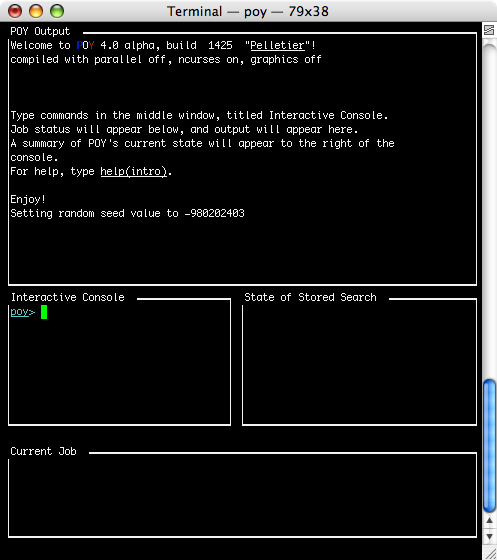
\includegraphics[width=0.9\textwidth]{doc/figures/figinterface.jpg}
\caption{\poy interface displayed in the Terminal window prior to analysis. 
Observe the cursor at the \poy prompt in the \emph{Interactive Console} 
and note that the \emph{State of Stored Search} and \emph{Current Job} 
windows are empty.}
\label{fig:figinterface}
\end{figure}

\begin{description}
%\setlength{\labelwidth}{0pt}
\setlength{\labelsep}{5pt}
\setlength{\itemindent}{0pt}%
\item[POY Output] (Figure \ref{fig:figinterface}, upper box) displays the 
status of the imported data, outputs the results of the phylogenetic analyses 
(such as trees, character diagnoses, and implied alignments), reports errors, 
and displays descriptions of \poy commands.
\item[Interactive Console] (Figure \ref{fig:figinterface}, mid-left box) 
is used to issue the commands interactively and to execute the commands 
by clicking the Return key. (See Section~\ref{commands} on the description 
of \poy commands.)
\item[State of Stored Search] (Figure \ref{fig:figinterface}, mid-right box) 
displays the time (in seconds) elapsed since the initiation of the current 
operation. This window also reports the number of trees currently in m
emory and displays the range of their costs.
\item[Current Job] (Figure \ref{fig:figinterface}, lower box) describes the 
currently running operation. When the operation is completed, the box is blank.
\end{description} 

\begin{figure}[htbp]
\centering
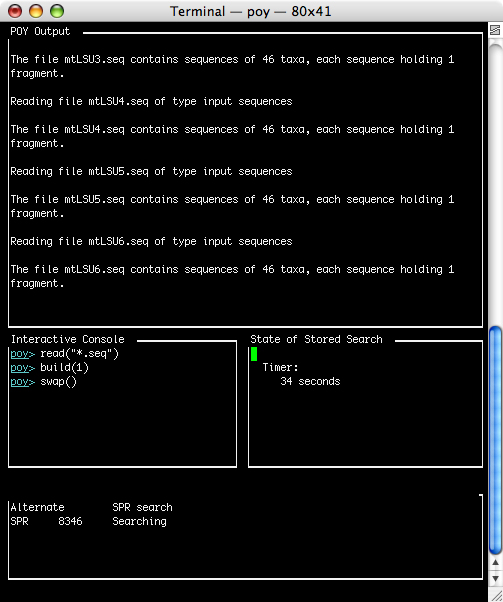
\includegraphics[width=0.9\textwidth]{doc/figures/figprocess.jpg}
\caption{\poy \emph{Interactive Console} during a process. The \emph{POY Output} 
window displays (by default) the information on the input data files. The 
\emph{Interactive Console} lists the commands that have been executed. The 
\emph{Current Job} window shows the state of the current operation and the 
current tree score. The \emph{State of Stored Search} shows the time elapsed  
since the last command \commandstyle{swap}, was initiated.}
\label{fig:figprocess}
\end{figure}

\subsection{Starting a \poy session using the \emph{Interactive Console}}

\begin{flushleft}
\begin{minipage}[c]{0.074\textwidth}

\includegraphics[width=\textwidth]{doc/figures/figlogowindows.jpg}
\end{minipage}
\,
\begin{minipage}[t]{0.88\textwidth}
\subsubsection*{Windows}
\end{minipage}
\begin{itemize}
\item{Start$>$All Programs$>$POY$>$Interactive Console}
\end{itemize}

\begin{minipage}[c]{0.074\textwidth}

\includegraphics[width=\textwidth]{doc/figures/figlogomac.jpg}
\end{minipage}
\,
\begin{minipage}[t]{0.88\textwidth}
\subsubsection*{Mac OSX}
\end{minipage}
\begin{itemize}
\item {Double-click \poy application icon to start the program.}
\item {Select \emph{Run Interactive Console} from the
\emph{Analyses} menu.}
\end{itemize}		

\begin{minipage}[c]{0.074\textwidth}

\includegraphics[width=\textwidth]{doc/figures/figlogolinux.jpg}
\end{minipage}
\,
\begin{minipage}[t]{0.88\textwidth}
\subsubsection*{Linux}
\end{minipage}
\begin{itemize}
\item Add \texttt{/opt/poy5/Resources/} (or the location you plan to install) to your \texttt{PATH} and run
\texttt{ncurses\_poy} from a terminal.
\end{itemize}
\end{flushleft}

\subsection{Entering commands}
Once this \poy interface is opened, the cursor appears in the
\emph{Interactive Console} portion of the window and is ready to
accept commands. The \emph{Interactive Console} does not support
using the mouse and, as is true for most command-line applications,
the cursor can be moved using the left and right arrow keys, and
the Backspace (in Windows) or Delete (in Mac) keys are used to erase
individual characters to the left of the current cursor position.
To eliminate the need for retyping commands anew during a \poy
session, keyboard shortcuts can be used: control-p (``previous'')
and control-n (``next'') will scroll through the commands previously
entered during the session. In addition, the \emph{Interactive
Console} is equipped with the autocomplete feature: it involves
\poy predicting a command, an argument, of file name that the user
wants to type from the first letter(s) entered. Upon typing the
first letter or part of the phrase, repeatedly pressing the TAB key
scrolls through the list of command, argument, and file names that
begin with that letter or phrase. Autocomplete simplifies interaction
with the program.

\subsection{Browsing the output}
As output is reported in the \emph{POY Output} window, only the
most recent reports will be seen in the window.  Using the Up and
Down keys allows the user to scroll up and down the \emph{POY Output}
window to see the welcome line, and previously printed reports and
help descriptions. Pressing Up and Down keys automatically places
the cursor in the lower left corner of the \emph{POY Output} window
indicating that you are interacting with that window. Only 1000
lines are stored in the memory and the output that was reported
before that will not be accessible by scrolling. The number of
lines, however, can be modified by the user using the command
\poycommand{set()}, see~\ccross{history}. If the user desires to
keep the entire output or specific items in the output, a log can
be created using the command \poycommand{set()}, see~\ccross{log})
or specific outputs can be redirected to files (see~\ccross{report}).
The user should be aware that outputting a log file can slow down
the program due to IO (input/output) delay.

\subsection{Switching between the windows}
To return to the \emph{Interactive Console}, start typing and the
cursor will automatically be placed back at the \poy prompt.  When
an operation is in progress (shown in the \emph{Current Job} window),
the cursor stays in the upper left corner of the \emph{State of
Current Search} window, and switching between the \emph{Interactive
Console} and the \emph{POY Output} window is disabled. There are
no user interactions in the \emph{Current Job} or \emph{State of
the State of Current Search}.

\subsection{Input of data} \label{sec:import}

The basic command to input data in \poy is \commandstyle{read()},
which includes the list of files (in quotation marks and separated
by commas) enclosed in parentheses. Suppose that we would like to
simultaneously analyze morphological and molecular datasets, contained
in separate data files, \texttt{morpho.ss} and \texttt{28s.fas},
respectively. We can issue a pair of \commandstyle{read()} commands
(Figure~\ref{fig:readingexample}): 

\begin{quote}
\commandstyle{read("morpho.ss")}\\ 
\commandstyle{read("28s.fas")}
\end{quote}

\begin{figure}
\begin{center}
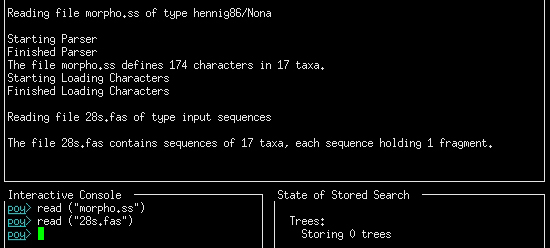
\includegraphics[width=0.9\textwidth]{doc/figures/reading_example.jpg}
\end{center}

\caption{Importing data files using the \emph{Interactive Console}.
Two consecutive \commandstyle{read} commands specify both the
morphological data file in Hennig86 format (\texttt{morpho.ss}),
and the molecular data file in FASTA format (\texttt{28s.fas}).
Observe that \poy automatically reports  in the \emph{POY Output}
window the names and types of files that have been imported.}
\label{fig:readingexample} \end{figure}

The syntax of \commandstyle{read}, like every command in \poy,
contains two elements: the name of the command, in this case
\commandstyle{read}, followed by an optional list of arguments
separated by commas and enclosed in parentheses. All filenames read
into \poy should include the appropriate suffix for the file type
(e.g. .fas, .ss, .aln, .tre etc:).  Typically, the arguments of the
command \commandstyle{read()} are names of data files, each being
enclosed in double quotes (as shown in the example above). Even
though there might be only one argument or none in some commands,
parentheses (e.g. \poycommand{pwd()}) always follow the command
name. An exhaustive discussion of \poy command structure and detailed
descriptions of all commands with examples of their usage are
provided in the \emph{POY Commands} chapter (\ref{commands}).

In order to import data by entering the names of the files, the
directory containing these files must be identified.  This can be
established in two ways--by using the command \commandstyle {cd}
to redirect the path to the directory where the data are found and
then reading in the data file:\\ 

\begin{quote}
\commandstyle{cd("/Users/username/docs/poyfiles")}\\
\commandstyle{read("28s.fas")}\\ 
\end{quote} 

or by including the
full path in the argument of \commandstyle{read}:\\ 

\begin{quote}
\commandstyle{read("/Users/username/docs/poyfiles/28s.fas")}
\end{quote}

Most of the time users are interested in importing multiple data
files to analyze an entire dataset. In this case, multiple data
files can be specified as arguments for a single command. For
example, importing both files, \texttt{morpho.ss} and \texttt{28s.fas},
can be written more succinctly:\\ \begin{quote}
\commandstyle{read("morpho.ss","28s.fas")} \end{quote} or if the
full path is included in the argument of \commandstyle{read} as:
\\

\begin{quote}
\commandstyle{read("/Users/username/docs/poyfiles/morpho.ss", \\
"/Users/username/docs/poyfiles/28s.fas")}
\end{quote}

This is equivalent to sequentially importing each file as shown in
(Figures ~\ref{fig:readingexample} and \ref{fig:reading_example2}).

Figures~\ref{fig:readingexample} and \ref{fig:reading_example2}
also illustrate an important feature that makes \poy different from
many other phylogenetic analysis programs: every time a file is
imported during a \poy session, the input data are \emph{added} to
the data in memory and \emph{do not replace them}. This
allows additional analytical flexibility. For example, if only
morphological data are read and trees are built based on these data
alone, a subsequently imported molecular character dataset will be
used in conjunction with the previously imported morphological data,
despite the fact that current trees in memory were generated only
from morphological data (Figure~\ref{fig:reading_example2}):

\begin{quote}
\commandstyle{read("morpho.ss")}\\
\commandstyle{build()}\\
\commandstyle{read("28s.fas")}\\
\commandstyle{rediagnose()}\\
\commandstyle{swap()}
\end{quote}

\begin{figure}[]
\begin{center}
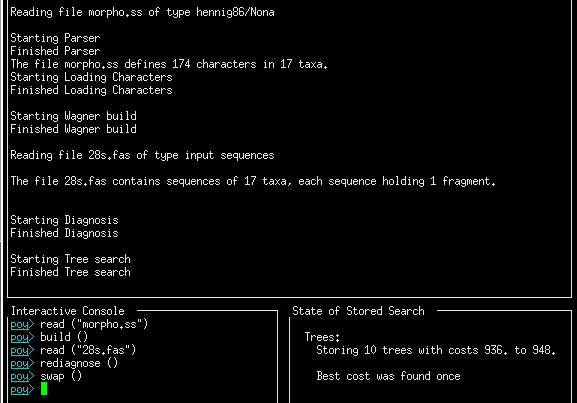
\includegraphics[width=0.9\textwidth]{doc/figures/reading_example2.jpg}
\end{center}
\caption{Building trees with morphological data only but continuing
the analysis using combined morphological and molecular data. This
example shows how we can add data to the analysis incrementally by
loading files at different points in the search. First, the
morphological data are imported from \texttt{morpho.ss} file using
\poycommand{read()} and trees are built based on these data.
Then molecular data from the \texttt{28s.fas} file are loaded into
memory. Finally, subsequent analyses, \commandstyle{rediagnose()} and
\commandstyle{swap()}, are conducted using all the data in memory, that
is the trees based on morphological data, and both morphological
and molecular character sets.} \label{fig:reading_example2}
\end{figure}

It must be noted that if the numbers of terminals differ among data
files, \emph{only} the data that correspond to the terminals used
to generate the trees (in this case, the morphological data file)
are used. The rest of the character data are ignored, unless the
trees are built again with the data files containing the expanded
number of terminals.  Also, because \poy appends trees and data in
memory, it is a good practice when starting a new analysis within
the same interactive session to clear the data using the command 
\commandstyle{wipe()}.

Valid input files include nucleotide and amino acid sequence files
in many formats, and morphological data in Hennig86 and Nexus
formats. (For information on specific formats supported by \poy and
other types of input files see ~\ccross{read}.)

\subsection{Inspecting data}

Once a dataset (or multiple datasets) is imported, \poy automatically
reports a brief description of contents for each loaded file in the
\emph{POY Output} (Figure ~\ref{fig:readingexample}). However, it
may be desirable to inspect the imported data in greater detail to
ensure that the format and contents of the files have been interpreted
correctly. This practice helps avoid common errors, such as
inconsistently spelled terminal names, which may result in bogus
results, produce error messages, and aborted jobs.

The basic command for outputting information is \commandstyle{report()}.
One of its arguments, \commandstyle{data}, outputs a set of tables
showing the list of terminals, the number and types of characters,
and the lists of terminals and characters excluded from the analysis.
To produce a report of the data files that were used in the previous
example (\texttt{morpho.ss} and \texttt{28s.fas}), we import the
data and execute \commandstyle{report(data)}:

\begin{quote}
\commandstyle{read("morpho.ss","28s.fas")}\\
\commandstyle{report(data)}
\end{quote}

This will generate an extensive, detailed output, partial views of
which are shown in Figure ~\ref{fig:reportdata}.  Obviously, the
entire report will not be visible in the \emph{POY Output} window.
Therefore, the Up and Down arrow keys and Page Up and Page Down
keys can be used to scroll.  By default, \poy reports the results
of executed commands to the \emph{POY Output} window. However, the
same output can be redirected to a file simply by adding the name
of the output file in the list of argument of the command
\commandstyle{report()} \emph{before} the argument specifying the
type of the requested report (in this case \commandstyle{data}, see
the command~\ccross{report} ). For instance, to output the data
into the file \texttt{data\_analyzed.txt} we would enter:

\begin{quote}
\commandstyle{read("morpho.ss","28s.fas")}\\
\commandstyle{report("data\_analyzed.txt",data)}
\end{quote}

\begin{figure}
\centering
\begin{minipage}[c]{0.52\textwidth}
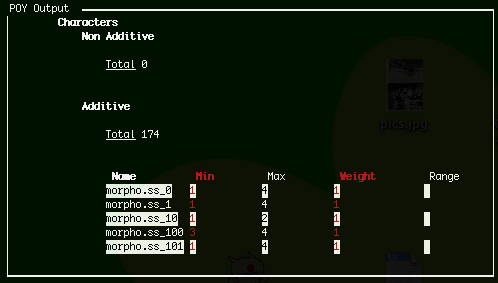
\includegraphics[width=\textwidth]{doc/figures/report2.jpg}
\end{minipage}
\,
\begin{minipage}[c]{0.44\textwidth}
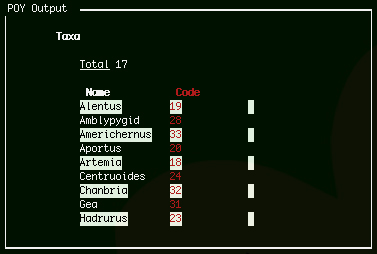
\includegraphics[width=\textwidth]{doc/figures/report3.jpg}
\end{minipage}
\caption{Inspecting imported data. The figure shows segments of 
a data report generated by \commandstyle{report(data)}. 
The left and right panels demonstrate a typical table output 
the character and terminal data respectively.}
\label{fig:reportdata}
\end{figure}

In this example, all the imported data are analyzed and, therefore,
the report fields that list excluded data will appear empty.  One
can, however, exclude specific characters or terminals from the
analysis using additional commands (see the command~\ccross{report}).

Another useful argument of \commandstyle{report} is
\commandstyle{cross\_references}. This argument displays whether
character data are present or absent for each terminal in each one
of the imported data files. This provides a comprehensive visual
overview of missing data. Building on the previous example, such
output can be generated by the following sequence of commands:
\begin{quote} \commandstyle{read("morpho.ss","28s.fas")}\\
\commandstyle{report("cross\_refs.txt",cross\_references)} \end{quote}

\begin{figure}[]
\begin{center}
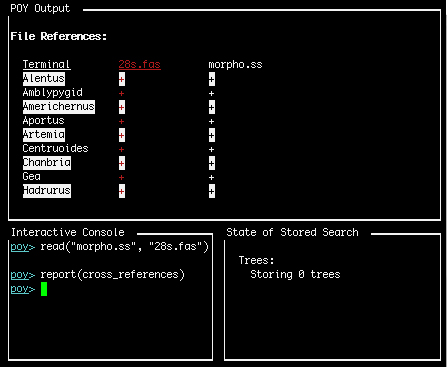
\includegraphics[width=1.0\textwidth]{doc/figures/crossref.jpg}
\end{center}
\caption{Visualizing missing data. The command
\commandstyle{cross\_references} displays a table showing whether
a given terminal (in the left column) is present (``+'') or absent
(``--'') in each data file. In this example, \texttt{28s.fas} is
missing for Amblypygid and \texttt{morpho.ss} for Hypochilus.}
\label{fig:crossref} \end{figure}

A typical output of \commandstyle{cross\_references} command is
shown in Figure ~\ref{fig:crossref}. This argument is a very useful
tool for visual representation of missing data. Moreover, reporting
all the data to a cross references file can also highlight
inconsistencies in the spelling of taxon names in different data
files.

\subsection{Building the initial trees}

The command to build trees is \commandstyle{build()} (already
mentioned in Section~\ref{sec:import}). After importing \texttt{morpho.ss}
and \texttt{28s.fas}, executing the command \commandstyle{build()}
without specifying any arguments (default settings) generates 10
Wagner trees by random addition sequence.

Many \poy commands operate under default settings when executed
without arguments. To learn what the default settings are for a
particular command use either the \commandstyle{help()} command with
the command name of interest inserted in parentheses or consult the
\emph{POY Commands} chapter (\ref{commands}).

If the user would like to specify a number of tree building replicates
different from the default value of 10, the argument \commandstyle{trees}
followed by a colon (``:'') and an integer specifying the number
of trees must be included in the argument list of the \commandstyle{build}
command: \commandstyle{build(trees:100)}. This command has a shortcut
that omits the argument \commandstyle{trees}. Thus,
\commandstyle{build(trees:100)} is equivalent to \commandstyle{build(100)}.
As defaults, the shortcuts are fully described in Section \ref{commands}.
The entire sequence of commands minimally required to import the
data and build 100 trees is the following:

\begin{quote}
\commandstyle{read("morpho.ss","28s.fas")}\\
\commandstyle{build(100)}
\end{quote}

As the tree building advances, the \emph{Current Job} window displays
the current status of the operation (Figure~\ref{fig:building}).
This window shows how many Wagner builds have been performed out
of the total number requested, the number of terminals added in the
current build, the cost of the current tree (recalculated after
each terminal addition), and the estimated time for the completion
of all the builds. When all the trees are generated, the \emph{State
of Stored Search} window displays the range of tree costs (the best
and worst costs), the number of trees stored in memory, and the
number of trees with the best cost (Figure~\ref{fig:building}).

\begin{figure}
\centering
\begin{minipage}[c]{0.507\textwidth}
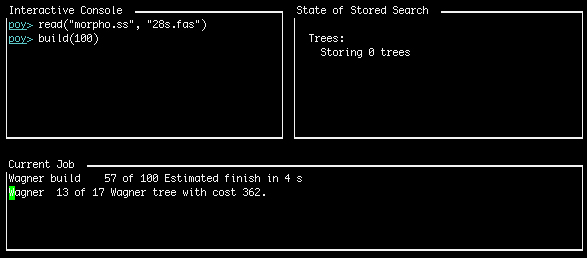
\includegraphics[width=\textwidth]{doc/figures/building1.jpg}
\end{minipage}
\,
\begin{minipage}[c]{0.453\textwidth}
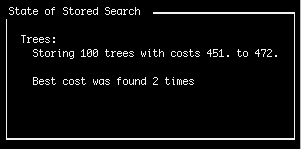
\includegraphics[width=\textwidth]{doc/figures/building2.jpg}
\end{minipage}
\caption{Generating Wagner trees. During the process of tree building (left 
panel), the \emph{Current Job} window displays how many builds have
been performed so far (\texttt{57 of 100}), the number of terminals
added in the current build (\texttt{13 of 17}), the cost of a current
tree recalculated after each terminal addition (\texttt{362}), and 
the estimated time (in seconds) for the completion of the operation
(\texttt{4 s}). Because the process is not complete, the \emph{State
of Stored Search} window contains no trees. Once tree building is
complete, the \emph{State of Stored Search} window displays the
best (\texttt{451}) and worst (\texttt{472}) costs, the number of
trees stored in memory (\texttt{100}), and the number of trees with
the best cost (\texttt{2}).} 
\label{fig:building}
\end{figure}

\subsection{Performing a local search}

Now that the trees have been generated and stored in memory, a local
search can be performed to refine and improve the initial trees by
examining additional topologies of potentially better cost.  The
command \commandstyle{swap()} implements an efficient strategy by
performing SPR and TBR branch swapping alternately. As with other
commands, the arguments of \commandstyle{swap()} allow the customization
of the swap algorithm. In the following example, branch swapping
is performed under the default settings on each of the 100 trees
build in the previous step:

\begin{quote}
\commandstyle{read("morpho.ss","28s.fas")}\\
\commandstyle{build(100)}\\
\commandstyle{swap()}
\end{quote}

Branch swapping is performed sequentially on all trees stored in
memory. During swapping, the \emph{Current Job} window reports the
number of the tree that is currently being analyzed, the method of
branch swapping, the specific routine being currently performed,
and the cost of the current tree (Figure~\ref{fig:swapping}). When
the process is complete, the \emph{State of Stored Search} window
displays the range of tree costs (the best and worst costs), the
number of trees stored in memory, and the number of trees with the
best cost (Figure~\ref{fig:swapping}). Notice that the local search
had reduced the costs of the initial best (from 451 to 446) and
narrowed the range of tree costs.

\begin{figure}
\centering
\begin{minipage}[c]{0.49\textwidth}
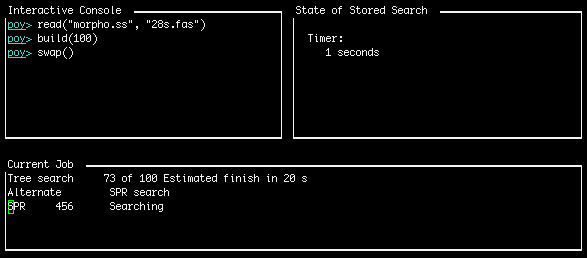
\includegraphics[width=\textwidth]{doc/figures/swap1.jpg}
\end{minipage}
\,
\begin{minipage}[c]{0.453\textwidth}
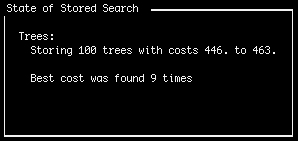
\includegraphics[width=\textwidth]{doc/figures/swap2.jpg}
\end{minipage}
\caption{Performing a local search. When searching (left panel),
the \emph{Current Job} window reports the number of the tree that
is currently being analyzed (\texttt{73 of 100}), a method of branch
swapping (\texttt{Alternate}), a function being currently performed
(\texttt{SPR search}), and a cost of the current tree (\texttt{456}).
When the searching is finished (right panel), the \emph{State of
Stored Search} window displays the best (\texttt{446}) and worst
(\texttt{463}) costs, the number of trees stored in memory
(\texttt{100}), and the number of trees of the best cost (\texttt{9})
recovered from independent tree builds and swaps. Notice that these trees may
not necessarily have unique topologies.}
\label{fig:swapping}
\end{figure}

Using different combinations of \commandstyle{swap()} arguments
allow the designation of a  large number of search strategies with
different levels of complexity. Some simple options allow the choice
between SPR and TBR. More complex strategies allow keeping a specific
number of best trees per single initial tree (generated during the
building step).  For example, the command \commandstyle{swap(trees:10)}
will keep up to 10 best trees generated during branch swapping on
a single initial tree. Consequently, if 100 trees were built
initially, this command will produce up to 1,000 trees. The argument
\commandstyle{threshold} allows the retention of suboptimal trees
within a specified percent of cost difference from the current best
tree. For example, \commandstyle{swap(trees:20,threshold:10)} will
execute a swap considering trees within a ten percent cost difference
of the current best tree and retain the 20 minimal length swapped
trees for each initial build. Other options provide the means to
sample trees as they are evaluated, timeout after certain number
of seconds, transform the cost regime, and other functions in
conjunction with many \poy commands.

\subsection{Selecting trees}

Having performed the basic steps of importing character data,
building initial trees, and conducting a simple local search, we
obtained a set of locally optimal trees in memory. Generally, a user
would like to select only those trees that are both optimal \emph{and}
topologically unique. The default setting of the \commandstyle{select()}
does exactly that.  Adding \commandstyle{select()} to our example
of command sequence for the basic analysis

\begin{quote}
\commandstyle{read("morpho.ss","28s.fas")}\\
\commandstyle{build(100)}\\
\commandstyle{swap()}\\
\commandstyle{select()}
\end{quote}

selects only unique trees of best cost. The remaining trees are
deleted from memory. The \emph{State of Stored Search} window reports
the number and the cost of the best tree(s) (Figure~\ref{fig:select}).

As an alternative, the user may choose to select topologically
unique trees, regardless of the cost, using \texttt{select(unique)}.
This may ensure that a larger tree space is explored.  If this is
used as an option during the search, the user should remember to
\commandstyle{select()} at the end of the run, prior to reporting
the results.

\begin{figure}[]
\begin{center}
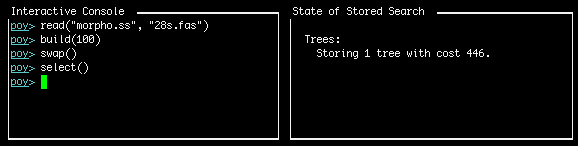
\includegraphics[width=0.9\textwidth]{doc/figures/select.jpg}
\end{center}
\caption{Selecting unique best trees. Executing \commandstyle{select()} 
keeps only unique trees of best cost. The \emph{State of Stored Search} 
window reports that there is only one unique tree of best cost (\texttt{446}).}
\label{fig:select}
\end{figure}

The command \commandstyle{select()}, is another multifunctional
command the arguments of which are also used to select (include or
exclude) specific terminals, characters, and trees.) Comparing the
output reported in the \emph{State of Stored Search} before
(Figure~\ref{fig:swapping}) and after (Figure~\ref{fig:select})
executing \commandstyle{select()} shows that swapping on 9 of 100
initial trees produced the trees of best cost (\texttt{446}), but
these trees are identical, because only one was retained when
filtered using \commandstyle{select()}.

\subsection{Visualizing the results}

There are several options for visualizing results in \poy
(see~\ccross{report}). The command \commandstyle{report("my\_first\_tree",graphtrees)} 
outputs a cladogram in PDF format (Figure~\ref{fig:trees}),
which can be displayed, edited, and printed using graphics software
(such as Adobe Illustrator or Preview).  \poy also appends the
``pdf'' extension when generating graphic output to a file. A quick
way to see the tree(s) on screen is to use the command
\commandstyle{report(asciitrees)} that draws a cladogram in the
\emph{POY Output} window (Figure~\ref{fig:trees}). The ascii tree(s)
can also be reported to a file, if an output file name is specified
within the command (\commandstyle{report("my\_first\_trees",
asciitrees)}).  These trees will be saved to a text file.

The command \commandstyle{report("my\_first\_trees.txt",trees)}
reports the trees in memory in parenthetical notation to the file
\texttt{my\_first\_trees} that can be imported in other programs.
Supported tree output formats include Newick and Hennig86.
\commandstyle{report()} can also generate consensus trees in the
graphical and parenthetical formats when appropriate arguments are
specified (for example, \commandstyle{report("strict\_consensus",graphconsensus)}).

\begin{figure}
\centering
\begin{minipage}[c]{0.45\textwidth}
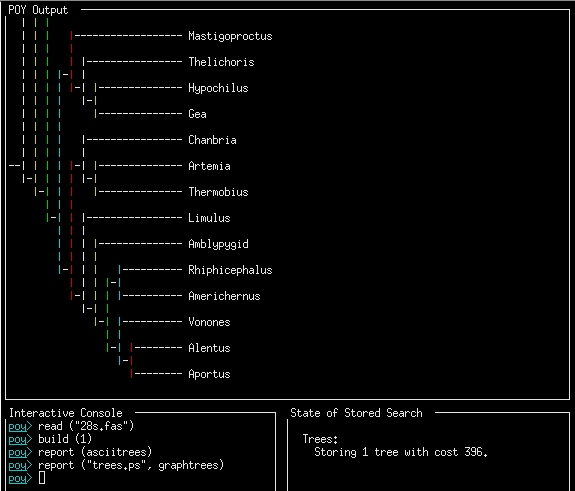
\includegraphics[width=\textwidth]{doc/figures/asciitrees.jpg}
\end{minipage}
\,
\begin{minipage}[c]{0.5\textwidth}
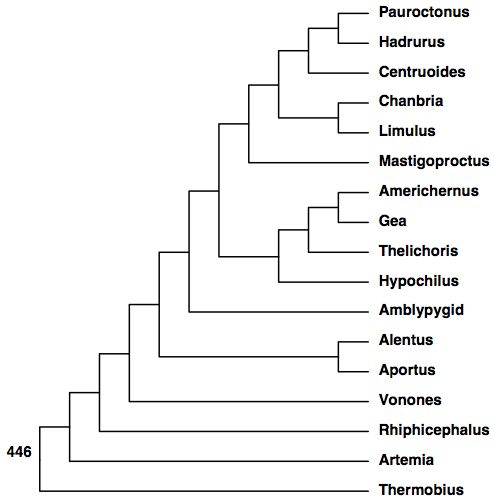
\includegraphics[width=\textwidth]{doc/figures/pstree.jpg}
\end{minipage}
\caption{Visualizing trees. An ascii tree (left) is generated using the command
\poycommand{report(asciitrees)}. The same tree is reported to a file in a PDF 
format (right) using \commandstyle{report("my\_first\_tree",graphtrees)}. 
Observe that both representations of trees  are preceded by their costs.}
\label{fig:trees}
\end{figure}

\subsection{Interrupting a process}
To interrupt a process, press control-c. By default, an error,
\texttt{Error:}\\ \texttt{Interrupted}, is reported in the \emph{POY
Output} window. The program does not close, however, and a new
command can be entered. Interrupting the analysis cancels the
execution of the last command requested by the user and restores
the data and trees in memory before that last command. For example,
the following two session are equivalent:

\begin{quote}
\commandstyle{read("morpho.ss") <ENTER>} \\
\end{quote}
and

\begin{quote}
\commandstyle{read("morpho.ss") <ENTER>} \\
\commandstyle{read("28s.fas") <CONTROL-C>} \\
\end{quote}

In both of these sessions, only the morphological dataset \texttt{``morpho.ss''} 
is read into \poy.

\subsection{Reporting errors}
If there is an error pertaining to incorrect syntax (such as a typo in a command 
name), \poy will indicate the location of the error by underlining the problematic 
part of the input with a hat symbol (``\texttt{\^}'') in the \emph{Interactive Console} 
(Figure~\ref{fig:errors}). The description of the corresponding command, its syntax, 
and examples of its usage from the help file are automatically printed in the 
\emph{POY Output} window. As noted above, the Up and Down keys can be 
used to scroll through the output and determine the source of the error. Certain 
types of errors are reported explicitly (Figure~\ref{fig:errors}).

\begin{figure}
\centering
\begin{minipage}[c]{0.48\textwidth}
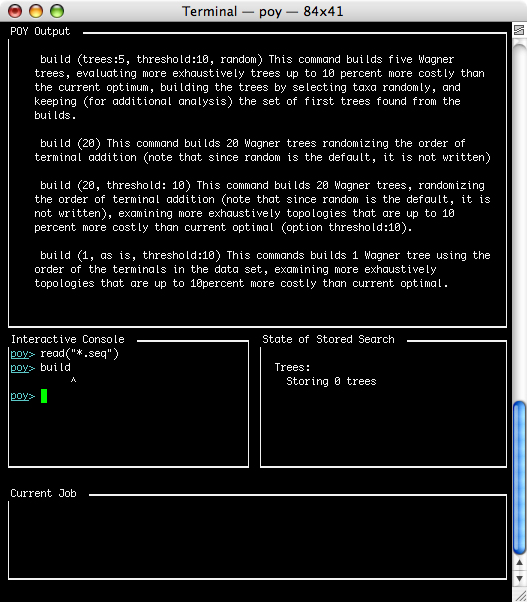
\includegraphics[width=\textwidth]{doc/figures/figerror1.jpg}
\end{minipage}%
\,
\begin{minipage}[c]{0.48\textwidth}
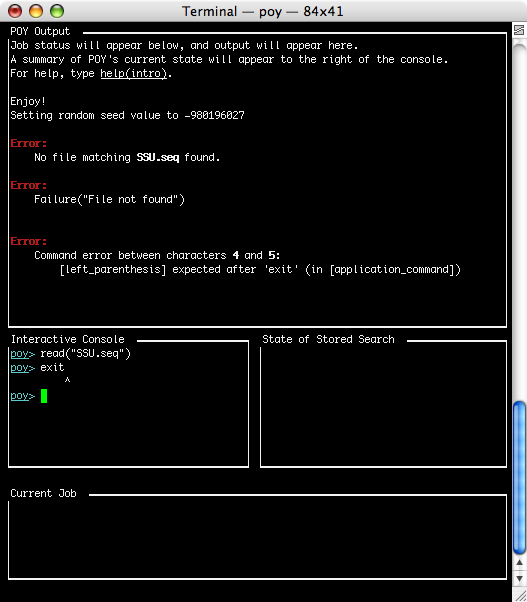
\includegraphics[width=\textwidth]{doc/figures/figerror2.jpg}
\end{minipage}
\caption{Displaying errors. \poy displays error messages in several
ways. In the example in the left panel, the command \commandstyle{build}
was entered without parentheses, which is required for a  valid
\poy command syntax; the exact place of the error is marked by
``\texttt{\^}'', in this case  following the \commandstyle{build}
commands. Examples of the proper usage of the command are automatically
displayed in the \emph{POY Output}.  In other cases (right panel),
error messages are explicitly reported in the \emph{POY Output}
window. The first and second error messages indicate that the data
file \texttt{SSU.seq} is not present, which could have been caused
either by a mistake in the name of the file, or missing file, or the
location of the file in a directory, other than the one specified
prior to starting the \poy session. The third error message indicates
that the valid syntax of \commandstyle{exit} requires the parentheses
following the command name (also shown by ``\texttt{\^}'' in  the
\emph{Interactive Console}).} \label{fig:errors} \end{figure}

\subsection{Exiting} To finish a \poy session, enter the command
\commandstyle{exit()} (Figure~\ref{fig:exithelp}) or \commandstyle{quit()}.
This will close the \poy interface and resume the Terminal window
(Mac OSX) or the Command Prompt window (Windows).

\begin{figure}[]
\begin{center}
\includegraphics[width=0.7\textwidth]{doc/figures/exithelp.jpg}
\end{center}
\caption{Exiting \poy}
\label{fig:exithelp}
\end{figure}

\section{Creating and running \poy scripts}

So far, we have communicated with \poy interactively through the
\emph{Graphical User Interface} or by executing commands from the
\emph{Interactive Console}. Another way of conducting an analysis
is to run a \emph{script}, a simple text file containing a list of
commands to be performed (Figure~\ref{fig:script}).

Running analyses using scripts has many advantages: not only does
it allow for the entire analysis to proceed from the beginning to
the end at one click of a button, but it also provides means to
examine the logical dependency of the commands and optimize memory
consumption (see the description of \poyargument{script\_analysis}
argument of the command \poycommand{report} in the \emph{POY Commands}
chapter). Submitting jobs using scripts may produce results faster
because \poy automatically optimizes the workflow of the entire
analysis by taking into account the functional relationships among
various tasks and efficiently distributing the jobs and resources
(such as memory and multiple processors).

Another advantage of using scripts is that they may contain comments
that are ignored by \poy but can be helpful to describe the contents
of the files and provide other annotations. The comments are enclosed
in parenthesis \emph{and} asterisks, e.g. \texttt{(* this is a
comment *)}. Comments can be of any length and span multiple lines.

Obviously, using scripts requires the user to design the workflow
of the process prior to conducting the analysis.  \poy scripts can
be created and saved using the \emph{Script Editor} window of the
\poy \emph{Graphical User Interface} or any conventional text editor
(such as TextPad, TextWrangler, BBEdit, Emacs, or NotePad).

\poy scripts are extremely useful in cases when operations may take
a long time to complete, eliminating the need to wait for a part
of the analysis to finish in order to proceed to the next step.
Moreover, scripts can contain a series of individual scripts that 
are run sequentially (see for example tutorial \texttt{5.4}.

There are two ways to import and run a script:
\begin{itemize}
\item using the \emph{POY Launcher} in the \emph{Graphical User Interface};
\item using the command \commandstyle{run()} of the \emph{Interactive Console}; 
for example, \texttt{run("script.txt")}, where \texttt{script.txt} is the name of 
the file containing the script. Within this script it is also possible to specify 
additional scripts to run.
\end{itemize}

It is  critical to include the command \commandstyle{exit()} at the
end of the script. Otherwise \poy will be waiting for further
instructions to be entered after executing the script's contents.

\begin{figure}
\centering
\begin{minipage}[c]{0.42\textwidth}
\includegraphics[width=\textwidth]{doc/figures/commandlist.jpg}
\end{minipage}
\,
\begin{minipage}[c]{0.53\textwidth}
\includegraphics[width=\textwidth]{doc/figures/script.jpg}
\end{minipage}
\caption{Using \poy scripts. The list of commands executed interactively
using the \emph{Interactive Console} (left) and a script containing
the same list of commands (right). Observe that the header of the
script is a comment, enclosed in ``(* *)'', that is ignored by \poy.
Also note that commands can either be listed in a row or in a column
(compare \commandstyle{build()} and \commandstyle{swap()} in the
console and in the script) and different arguments of the same
command can either be specified separately or combined in a single
argument list (compare \commandstyle{report()} in the console and
in the script). (Both conventions are valid for interactive command
submission and for scripts.)} 
\label{fig:script}
\end{figure}

\section{Obtaining help} \label{sec:help} 
Instructions to run \poy, command descriptions, and the theory behind \poy can be obtained
from a variety of sources.  

\begin{description} 
\item[POY5.0 Program Documentation] (this manual) is a comprehensive 
and detailed manual on all the aspects of using \poy, from installation to 
output and visualization of results. Included are \emph{Quick Start}, \poy
command reference, practical guides and tutorials that make the
program immediately accessible for beginners and provide in-depth
information for experienced users. As with any PDF, this document 
is easily searched using key words or phrases. The documentation in PDF format
can be accessed from the \emph{Help} menu of the graphical user
interface or downloaded separately from \poy web site at \begin{center}
\url{http://www.amnh.org/our-research/computational-sciences/research/projects/systematic-biology/poy/download}
\end{center} 
\item[POY] interactive help can be obtained by entering
\commandstyle{help()} at the \poy \emph{Interactive Console}.  To
obtain help on a particular command, the name of the command must
be specified in the parentheses following \commandstyle{help()}.
For example, to learn about the command \commandstyle{exit}, type
\commandstyle{help(exit)}.  (Figure~\ref{fig:exithelp}.) 
\item[POY5
Mail Group] is an Internet-based forum for discussing all issues
related to \poy and provides the best way to communicate with \poy
developers on specific issues (see \emph{WWW resources} below). The
website is located at \url{https://groups.google.com/forum/#!forum/poy4}.
Questions relating to both \texttt{POY4} and \poy can be posed to
this group.  
\item[POY Book] (Wheeler et al., 2006 \emph{Dynamic
Homology and Phylogenetic Systematics: A Unified Approach Using
POY} \cite{wheeleretal2006}) provides a review of the theory behind
\texttt{POY4} and by extension \poy, and contains formal descriptions
of many algorithms implemented in the program and the descriptions
of commands of the earlier version, \texttt{POY3}. A PDF version of 
the book is available at \url{http://research.amnh.org/scicomp/pdfs/wheeler/Wheeler_etal2006b.pdf} 
\item[POY Paper] (Var\'on et al., 2010. \emph{POY version 4: 
Phylogenetic analysis using dynamic homologies} \cite{Varonetal2010} 
provides a description of the overall goals, implementation and philosophy 
of POY.

\begin{figure}[htbp]
\centering
\includegraphics[width=0.23\textwidth]{doc/figures/figpoybook.jpg}
\caption{The POY Book.}
\label{fig:figprocess}
\end{figure}
\end{description}

\section{WWW resources}
\poy is an ongoing project and new versions are being continuously
developed to include new procedures, improve performance, and
eliminate reported bugs. Therefore, it is imperative to keep up
with the program's development and check regularly for updates.
There are several Internet-based resources that offer this information.

\begin{description}
\item[POY5 Web Site] Has downloadable compressed files of \poy
binaries, source code, and documentation in PDF format. It also
provides a links to the \emph{POY Mail Group}. The website is hosted
by AMNH Computational Sciences at \begin{center}
\url{http://www.amnh.org/our-research/computational-sciences/research/projects/systematic-biology/poy}
\end{center}

\item[POY5 source code repository] Contains has downloadable \poy
source code.  The site is powered by Google at \begin{center}
\url{http://code.google.com/p/poy/source} \end{center}

\item[POY5 Mail Group] Informs registered users via email of new
developments, such as new versions and updates.  It also provides
additional resources for obtaining help and a way for reporting
bugs and other problems with \poy and its documentation. In addition,
it allows users to receive and respond to each other's questions
thus providing an open forum to  discuss the methods and applications
of \poy. The users who choose not to register, have access to the
archives of the postings but will not be able to either submit or
receive emails from other users and \poy developers. The \emph{POY5
Mail Group} is hosted  by Google at \begin{center}
\url{https://groups.google.com/forum/#!forum/poy4} \end{center}

\end{description}

\chapter{\poy Commands}\label{commands}

\section{\poy command structure}

\subsection{Brief description} \label{commands}

\poy interprets and executes \emph{scripts} issued by the end user.  These can
come from the command line in the \emph{Interactive Console} of the program, or from an
input file. A script is a list of \emph{commands}, separated by any number of
whitespace characters (spaces, tabs, or newlines). Each command consists of a
name  in lower case (\poylident), followed by a list of arguments separated 
by commas and enclosed in parentheses. Most of the arguments are optional, in
which case \poy has default values.

In \poy, we recognize four types of command arguments: \emph{primitive values},
\emph{labeled values}, \emph{commands}, and \emph{lists of arguments}.

\paragraph{Primitive values} can be either an integer (\poyint), a real number
(\poyfloat), a string (\poystring), or a boolean (\poybool).

\paragraph{Labeled values} are a lowercase identifier (which are referred to as
\emph{label}), and an argument, separated by the colon character. ``:''.

\paragraph{List of arguments} are several arguments enclosed in parenthesis and
separated by commas, ``,''.

\paragraph{Commands} are standard commands that can affect the behavior of
another command when included in its list of arguments.

\paragraph{}Thus, certain commands can function as arguments of other commands. Moreover,
some commands share arguments. Although such compositive use of commands
might seem complex, this structure provides much more intuitive
control and greater flexibility. The fact that the same logical operation that functions
in different contexts maintains
the same name (typically suggestive of its function), substantially reduces the number of
commands without limiting the number of operations. Using a linguistic analogy,
\poy specifies a large number of procedures by a more complex grammar (specific
combinations of commands and arguments), rather than by increasing the vocabulary
(the number of specific commands and arguments). For example, the command
\poycommand{swap} specifies the method of branch swapping. This command is
used to conduct a local search on a set of trees. In addition,
\poycommand{swap} functions as an argument for \poycommand{calculate\_support}
to specify the branch swapping method used in each pseudoreplicate during Jackknife or
Bootstrap resampling. \poycommand{swap} can also be used to set the parameters for
local tree search based on perturbed (resampled or partly weighted) data as an argument
of the command \poycommand{perturb}. Therefore, to take the maximum advantage of
\poy functionality, it is essential to get acquainted with the grammar of  \poy.

\subsection{Grammar specification}

The following is the formal specification of the valid grammar of a script in \poy:

\begin{verbatim}
script: = | command
        | command script

command: = LIDENT "(" argument list ")"

argument list: = |
            | arguments

arguments: = |
            | argument
            | argument "," arguments

argument: = | primitive
            | LIDENT
            | LIDENT ":" argument
            | command
            | "(" argument list ")"

primitive: = | INTEGER
            | FLOAT
            | BOOLEAN
            | STRING

LIDENT: = [a-z_][a-zA-Z0-9_]*

INTEGER: = [0-9]+

FLOAT: = | INTEGER
        | [0-9]+ "." [0-9]*

STRING: = """ [^"]* """

\end{verbatim}

The following examples graphically show a typical structure of valid \poy commands
formally defined above. The Figure \ref{simplecommand} illustrates
the syntax of the command \poycommand{swap}. The name of the
command, \poycommand{swap}, is followed by a list of two arguments,
\poyargument{tbr} and \poyargument{trees:2}, inclosed in parentheses
and separated by a comma. Note that \poyargument{trees:2} is a labeled-value
argument that contains a label (\texttt{trees}) and a value (\texttt{2})
separated by a colon.

\begin{figure}[htbp]
   \centering
   \includegraphics[width=0.34\textwidth]{figures/fig-poycommand1.jpg}
   \caption{The structure of a simple \poy command. The entire command (highlighted
   in blue), consists of  a command name followed by a list of arguments (enclosed in red box).
   See text for details.}
   \label{simplecommand}
\end{figure}

Figure \ref{compositecommand} shows a more complex command structure, using the command \poycommand{perturb} as an example. This is a compound command because the list of its arguments contains another command, \poycommand{swap}. This means that executing \poycommand{perturb} performs a set of specified operations that contains a nested set of operations specified by \poycommand{swap}. Note also, that in contrast to the first labeled-values argument \poyargument{iterations}, the second labeled-values argument \poyargument{ratchet} has multiple values (a float and an integer). When multiple values are specified, they must be enclosed in parentheses and separated by a comma. The third argument is a command (\poycommand{swap}), therefore it is syntactically distinguished from other arguments, labeled and unlabeled alike, by having parentheses following the command name. It must be emphasized that the parentheses always follow the command name even if no arguments are specified. (If no arguments are specified, a command is executed under its default settings.)

\begin{figure}[htbp]
   \centering
   \includegraphics[width=0.8\textwidth]{figures/fig-poycommand2.jpg}
   \caption{A structure of a compound \poy command. Note that the list of arguments
   (enclosed in red box) includes a command (highlighted in blue). Also, note that
   \poyargument{ratchet} accepts multiple values, a float and an integer, that are inclosed in
   parentheses and separated by a comma. See text for details.}
   \label{compositecommand}
\end{figure}

\section{Notation}

Some arguments are obligatory, whereas others are not; some commands accept an
empty list of arguments, but others do not; some argument labels have
obligatory values, some have optional values. In the descriptions of
\poy commands below, the elements of \poy grammar are defined in
the text using the following conventions:

\begin{itemize}
    \item A command that could be included in a \poy script (that is can be entered in the
    	interactive console or included in an input file) is shown in \poycommand{terminal type}.
    \item Optional items are inclosed in \poycommand{[square brackets]}.
    \item Primitive values are shown in \poycommand{UPPERCASE}.
\end{itemize}

Each command description entry contains the following sections:

\begin{itemize}
    \item The name of the command.
    \item A brief description of the command's function.
    \item Cross references to related commands.
    \item The valid syntax for the command.
    \item The list of descriptions of valid arguments.
    \item Description of default settings.
    \item Examples of the command's usage.
\end{itemize}

\begin{statement}
    Default syntax. The default syntax for all commands is the same: it includes the
    command name followed by empty parentheses. For example,
    \poycommand{swap()}. The descriptions of default settings, however,
    include the entire argument list for the obvious reason of showing what is
    included in the omitted argument list.
\end{statement}

\begin{statement} \label{commandorder}
    Command order. The effect of the order of arguments in a command depends on the context. 
    If arguments are not logically interconnected, their order is not
    important. For example, the commands \poycommand{build(10,randomized)} and
    \poycommand{build(randomized,10)} are equivalent. However, executing the
    commands \poycommand{transform(tcm:(1,1),gap\_opening:4)} and
    \poycommand{transform(gap\_opening:4,tcm:(1,1))} will produce different results
    because \poycommand{gap\_opening} \emph{modifies} the values set by
    \poyargument{tcm}, while \poyargument{tcm} \emph{overrides} the values set by \poyargument{gap\_opening}.
\end{statement} 

\begin{statement}
    Output files. When an output file is specified, the file name (in double quotes and
    followed by a comma) must precede the argument.
\end{statement}

\begin{statement}
    Certain command arguments are mainly useful to \poy developers, and
    those arguments are preceded by an underscore.
\end{statement}

\section{Command reference}
   %build
   
     \begin{command}{build}{buildcommand}

    \syntax{\obligatory{(\optional{argument list})}}
	
 	\begin{poydescription}
        Builds Wagner trees~\cite{farris1970}. Building multiple trees with a randomized addition of terminals allows for
        the evaluation of many more possible tree topologies and generates a diversity of trees for subsequent analysis. 
        The arguments of the command \poycommand{build} specify the number of trees to be generated and
        the order in which terminals are added during a single tree building procedure. During tree
        building, \poy reports in the \emph{Current Job} window of the \emph{ncurses} interface
        which of the terminal addition strategies (e.g. \texttt{as\_is} or \texttt{randomized}) is currently used.
        
        By default \poy replaces the trees stored in memory with those generated
        in a subsequent build. For example, executing \poycommand{build(10)}
        followed by \poycommand{build(20)} will replace the 10 trees generated
        during the first build with 20 new trees. However, it might be desirable
        to generate a large number of trees by
        appending trees from multiple separate builds. To keep trees from consecutive
        builds, a tree output file must be specified using the command ~\ccross{report} that must 
        precede the \poycommand{build} command. This will produce a file
        containing the trees appended from all builds. If the same file name is used for reporting
         trees for other analysis, the new trees are going to be appended. Alternatively, trees from different
        builds can be redirected to separate files if different file names are specified.
        
        The command \poycommand{build} is also used as
        an argument for the command \poycommand{calculate\_support}.
   	\end{poydescription}

\begin{arguments}

        \argumentdefinition{all}{\optional{\poyint}}
            {Turns off all preference strategies for adding branches
            and simply tries all possible addition positions for
            all terminals.  By default ten trees are built but the number 
            of  trees can be specified by the integer or by the argument 
            \poyargument{trees}.}
            {allbuild}

        \argumentdefinition{as\_is}{} 
            {Indicates that in one of the trees to be built, the terminals are
            added in the order in which they appear in the imported data files,
            and all others are built using a random addition sequence.}
            {asis}

        \argumentdefinition{branch\_and\_bound}{\optional{\poyfloat}}
            {Calculates the exact solution using the Branch and Bound algorithm
            ~\cite{hendy1982}. By default only one optimal tree is kept but
            the number of optimal trees to be retained can be specified by the
            argument \poyargument{trees}. The optional float value specifies the
            bound (either tree cost or likelihood score).}
            {branchandbound} 

        \argumentdefinition{constraint}{\optional{\poystring}}
            {Builds trees using the set of constraints specified by a consensus
            tree input file. If no input file is provided, the constraint is calculated as
            the strict consensus of the trees in memory. Every tree built
            using this method is subjected to the same randomization as Wagner
            builds within each constraint.}
            {buildconstraint}

        \argumentdefinition{INTEGER}{}
            {The integer argument specifies the number of independent, individual
            Wagner tree builds. This is a shortcut of the argument \poyargument{trees}.}
            {}

        \argumentdefinition{lookahead}{\obligatory{\poyint}}
            {The number of trees that can be kept at each build step. If the
            \poyargument{lookahead} argument 
            specifies a number $n$, and the best tree found has cost $c$, then the best $n$
            trees with cost at most $c + threshold$ as specified by
            the \nccross{threshold}{buildthreshold} command are held for the
            next build step. If no \poyargument{threshold} command is specified,
            then it is set to $0$.}
            {lookahead}

          \argumentdefinition{of\_file}{\obligatory{\poystring}}
            {Imports a tree file included in the file path of the argument. This command is
            useful for importing starting trees for calculating \ccross{bremer} support.
            In other contexts the command \ccross{read} can be used with the same effect.}
            {offile}

         \argumentdefinition{optimize} {(model \optional {\poylident}, branch\optional {\poylident})}
            {Specifies when the likelihood model and how the branches are optimized during
            the build routine. These options are also available in the \poycommand{fuse} and 
            \poycommand{swap} commands. In all cases a complete round 
            of optimization will occur after the completion of a build.

            \begin{description}

                  \argumentdefinition{model:always}{}
                    {Optimize the model after every additional taxon is added (default).}
                    {buildmodelalways}
                    
                \argumentdefinition{model:max\_count:{\poyint}}{}
                    {Optimize the model after every defined number (\poyint) of taxa are added to the tree.}
                    {buildmaxcount}
                    
                \argumentdefinition{model:never}{}
                    {Do not optimize the model during the build.}
                    {buildmodelnever}
\\
                \argumentdefinition{branch:all\_branches}{}
                    {Optimize all branch lengths after each taxon is added (default).}
                    {buildallbranches}

                \argumentdefinition{branch:join\_region}{}
                    {Optimize a maximum of five branches; the edge connecting
                    the new taxa to the tree, and the two sides of that joined
                    edge.}
                    {buildjoinregion}
                    
                \argumentdefinition{branch:never}{}
                    {Do not optimize the branches during the build process. We use
                    an estimate based on the proportion of sites that transform.}
                    {buildbranchnever}

            \end{description}
            }
            {buildoptimize}

	 \argumentdefinition{nj}{}
            {Creates a tree using the Neighbor Joining algorithm~\cite{saitou1987}. If more than
            one tree is requested, all the trees will be the same (the algorithm
            implementation is deterministic).}{}

        \argumentdefinition{random}{}
            {Generates a tree at random. All possible trees have equal probability.}
            {buildrandom}

	    \argumentdefinition{randomized}{} 
            {Indicates that terminals are added in random order on every Wagner tree built. 
            This is a default tree-building strategy.}
            {randomized}

       \argumentdefinition{STRING}{}
            {This is a shortcut of the argument \poyargument{of\_file}.}
            {}

        \argumentdefinition{threshold}{\obligatory{\poyfloat}}
            {The numerical value specifies the extra cost over the current best
            tree that makes another tree acceptable for the lookahead list. This 
            parameter is only useful if~\nccross{lookahead}{lookahead} is used.}
            {buildthreshold}
            
        \argumentdefinition{trees}{\obligatory{\poyint}}
            {The integer value specifies the number of independent, individual
            Wagner tree builds. The label \poyargument{trees} is optional: it is
            sufficient to specify only the integer value. Therefore, \poycommand{build(5)} is
            equivalent to \poycommand{build(trees:5)}.  Note that  \poyargument{trees} is
            also used as an argument of the command \nccross{swap}{swapcommand}
            but with different meaning.
            
            The value \texttt{0} generates no trees but it \emph{retains} all trees in memory.
            This is useful, for example, in the \ccross{bremer} support calculation,
            where instead of generating new trees per each node, the searches are
            performed on the trees in the neighborhood of the current trees in memory.}
            {treesbuild}
            

   \end{arguments}
      
   \poydefaults{trees:10, randomized, lookahead:1, threshold:0}
       {By default, \poy will build 10 trees using a random addition sequence for
       each of them.}

	\begin{poyexamples}
	\poyexample{build(20)}
            {Builds 20 Wagner trees randomizing the order of terminal
            addition (note that because the argument \poyargument{randomized} 
            is specified by default, it can be omitted).}
           
	\poyexample{build(trees:20, randomized)}
            {A more verbose version of the previous example. By default a build
            is randomized, but in this case the addition sequence is explicitly
            set. For the total number of trees, rather than simply specifying \texttt{20},
            the label \texttt{trees} is used. The verbose version might be desirable
            to improve the readability of the script.}

          \poyexample{build(all:30)}
            {Builds 30 Wagner trees, trying all possible addition positions for all terminals}.
            
	\poyexample{build(15, as\_is)}
            {Builds the first Wagner tree using the order of terminals in the first
            imported data file and generates the remaining
            14 trees using random addition sequences.}
            
           \poyexample{build(branch\_and\_bound, trees:5)}
            {Builds trees using branch and bound method and keeps up to
            5 optimal trees in memory.}
            
            \poyexample{build(constraint:"cstree.tre")}
            {Builds trees using using the set of constraints specified by the consensus tree 
            file "cstree.tre".}
            
            \poyexample{build(trees:100,optimize(model:max\_count:5,branch: \\  all\_branches))}
            {Builds 100 trees and optimizes the likelihood model after every 5 
            taxa are added to the tree.  All branch lengths are optimized after the addition 
            of each taxon to the tree.}
                    
	\end{poyexamples}

\end{command}

%calculate_support

\begin{command}{calculate\_support}{calculatesupport}

	\syntax{\obligatory{(\optional{argument list})}}

	\begin{poydescription} 
            Calculates the requested support values. \poy implements support
            estimation based on resampling methods (Jackknife~\cite{Farrisetal1996} 
            and Bootstrap~\cite{Felsenstein1985}) and Bremer support~\cite{Bremer1988, 
            Kallersjoetal1992}. The Jackknife and Bootstrap support values are computed as
            frequencies of clades recovered in strict consensus trees built in each resampling
            iteration. The consensus trees are based on best trees recovered in each replicate
            with zero-length branches collapsed. All the arguments of 
            \poycommand{calculate\_support} command are optional and
            their order is arbitrary.  For examples of scripts implementing support measures see 
           tutorials \texttt{5.4}, \texttt{5.5} and \texttt{5.6}. 
            
	  The \poycommand{calculate\_support} command does not output support 
	  values by default. The output of support values must be requested using 
	  the command~\ccross{report}. This is particularly important for Jackknife 
	  and Bootstrap support values, as these sampling techniques
            do not require the presence of trees in memory. Therefore, it is possible to 
            perform the sampling for support values \emph{before}
            the tree of interest has been found.
                    \end{poydescription}
            
 \begin{statement}

                In the context of dynamic
                homology, the characters being sampled during pseudoreplicates
                are entire sequence fragments, not individual nucleotides.
                Consequently, the bootstrap and jackknife support values
                calculated for dynamic characters are not directly comparable to
                those calculated based on static character matrices. If it is
                desired to perform character sampling at the level of
                individual nucleotides, the dynamic characters must be
                transformed into static characters using \poyargument{static\_approx}
                argument of the command~\ccross{transform}
                prior to executing \poycommand{calculate\_support}. Alternatively, an 
                output file in the Hennig86 format can be
                generated based on an implied alignment
                using~\ccross{phastwinclad} that can subsequently be analyzed
                using other programs.  
                
 \setlength{\parindent}{0.5cm}                                
                \indent Of course, 
                if the dataset of dynamic characters contains a large number of fragments, 
                this caveat may not be warranted.
                
 \setlength{\parindent}{0.5cm}                                
                \indent It is important to remember that the local optimum for the dynamic
                homology characters can differ from that for the static homology characters
                based on the same sequence data. Therefore, it is recommended to perform 
                an extra round of swapping on the transformed data to reach the local 
                maximum for the static homology characters prior to calculating support values.
            \end{statement}
          
 \begin{statement}
	The placement of the root affects calculation of Bremer support values.
	  Therefore, it is critical to specify the root prior to executing
	  \poycommand{calculate\_support}. See the description of the
	  command \nccross{set}{root} on how to specify the root.
	\end{statement}          
                       
        
              
	\begin{arguments}
		\begin{argumentgroup}{Support calculation methods}
            {The following commands allow selection among several methods for
            calculating support.} 

			\argumentdefinition{bootstrap}{\optional{\poyint}}
                {Calculates Bootstrap support~\cite{Felsenstein1985}. 
                The integer value specifies
                the number of resampling iterations (pseudoreplicates). If the value
                is omitted, 5 pseudoreplicates are performed by default.} 
                {}
                
			\argumentdefinition{bremer}{}
                {Calculates Bremer support values ~\cite{Bremer1988, Kallersjoetal1992}
                for each tree in memory by performing independent constrained searches for each
                node. The parameters for the searches can be modified using arguments
                described under \emph{Search strategy}.} 
                {}
  
			\argumentdefinition{jackknife}{\optional{([argument list])}}
                {Calculates Jackknife support~\cite{Farrisetal1996} using the 
                sampling parameters specified by the arguments. The arguments of
                \poyargument{jackknife} are optional and their order is arbitrary. If
                both values are omitted, the default values of each argument is used.}
                {}
        
              	        
                \begin{description}
                    \argumentdefinition{remove}{\obligatory{\poyfloat}}
                        {The value of the argument \poyargument{remove} specifies the
                        percentage of characters being deleted during a pseudoreplicate. The
                        default of \poyargument{remove} is \texttt{36} percent.}
                        {}
                     \argumentdefinition{resample}{\obligatory{\poyint}}
                        {The value of the argument \poyargument{resample} specifies the
                        number of resampling pseudoreplicates. The default of \\
                        \poyargument{resample} is \texttt{5}.}
                        {}
               \end{description}  
		\end{argumentgroup}

        \begin{argumentgroup}{Search strategy}
            {The calculation of the support values requires a local search,
            that is performed under the default settings unless the values
            of the following arguments are specified.}
		 
	     \argumentdefinition{build}{}
             {For calculating Bremer support, the integer value of
             \poyargument{build} specifies the number of independent
             Wagner tree builds per node. The integer value \texttt{0}
             (\texttt{build:0}) specifies that Bremer support values are
             calculated on the starting trees currently
             in memory, rather than on newly generated trees.
             The initial trees for calculating Bremer support
             can also be imported using the argument \poyargument{of\_file}
             of the command ~\nccross{build}{buildcommand}.
             
             For calculating Jackknife
             and Bootstrap supports, build specifies the number of
             Wagner tree builds per pseudoreplicate.  Single best trees from all
             pseudoreplicates are used to calculate the support values. If
             multiple best trees are recovered in a pseudoreplicate, one 
             is selected. If \poyargument{build} is
             omitted from the argument list of \poycommand{calculate\_support},
             a single random addition Wagner tree per
             pseudoreplicate is built by default. This is equivalent to 
             \poycommand{build(trees:1, randomized)}. See
             \nccross{build}{buildcommand} for a detailed discussion of
             arguments of the command \poycommand{build}.}
             {buildarg}

        \argumentdefinition{swap}{}
            {Specifies the method and parameters for local tree search. If search
            parameters are not specified, the search is performed under
            the default settings of ~\nccross{swap}{swapcommand}.} 
            {swaparg}
	     
        	\end{argumentgroup}

	\end{arguments}

    \poydefaults{bremer,build(trees:1,randomized),swap(trees:1)}
    {By default \poy will calculate the Bremer support for each tree in memory node by node.
    However, if no trees are stored in memory, executing the command
    \poycommand{calculate\_support()} does not have any effect.}
    
     	\begin{poyexamples} 

        \poyexample{calculate\_support(bremer)}
            {Calculates Bremer support values by performing
            independent searches for every node for every tree in memory. 
            This is equivalent to executing \poycommand{calculate\_support()}, the default setting.}
         
         \poyexample{calculate\_support(bremer, build(trees:0), swap(trees:2))}
            {Calculates Bremer support values by performing swapping on 
            each tree in memory for every node and keeping up to two
            best trees per search round.}
          
          \poyexample{calculate\_support(bremer, build(of\_file:"new\_trees"), \\
          swap(tbr, trees:2))}
            {Calculates Bremer support values by performing TBR swapping on 
            each tree in the file \texttt{new\_trees} located in the current
            working directory for every node and keeping up to two
            best trees per search round.}  
            
         \poyexample{calculate\_support(bootstrap)}
         {Calculates Bootstrap support values under default settings. This command
         is equivalent to \poycommand{calculate\_support(bootstrap:5, \\ build(trees:1,
         randomized), swap(trees:1))}.}
	
        \poyexample{calculate\_support(bootstrap:100, build(trees:5), \\
            swap(trees:1))}
            {Calculates Bootstrap support values performing one random resampling with
            replacement, followed by 5 Wagner tree builds (by random addition sequence)
            and swapping these trees under the default settings of the command 
            \poyargument{swap}, and keeping one minimum-cost tree. The procedure
            is repeated 100 times.}
        
        \poyexample{calculate\_support(jackknife)}
            {Calculates Jackknife support values under default settings.  This command
            is equivalent to \poycommand{calculate\_support(jackknife:(resample:5, \\
            remove:36), build(trees:1, randomized), swap(trees:1))}.}     
            
         \poyexample{calculate\_support(jackknife:(resample:1000, remove:25), \\ 
            build(100), swap(tbr,trees:5))}
            {Calculates Jackknife support values randomly removing 25 percent of the
            characters, building 100 Wagner trees by random addition sequence, swapping 
            these trees using \poyargument{tbr}, and keeping up to 5 minimum-cost tree in the
            final swap per swap (totaling up to 500 stored trees per replicate). 
            The procedure is repeated 1000 times.}

	\end{poyexamples}
            
	\begin{poyalso}
		\cross{report}
        \ncross{supports}{supports}
        \ncross{graphsupports}{graphsupports}
	\end{poyalso}

\end{command}

   %clear_memory
   
\begin{command}{clear\_memory}{clearmemory}

	\syntax{\obligatory{(\optional{argument list})}}
	
	\begin{poydescription}
            Frees unused memory. Rarely needed, this is a useful command when the
            resources of the computer are limited. The arguments are optional and
            their order is arbitrary.
	\end{poydescription}
	
	\begin{arguments}
		\argumentdefinition{m}{}
            {Includes the alignment matrices in the freed memory.} 
            {clearmemoryalign}

		\argumentdefinition{s}{}
            {Includes the unused pool of sequences in the freed memory.}
            {clearmemoryseq}
	\end{arguments}
	
    \poydefaults{}{By default \poy clears all memory
    \emph{except} for the pool of unused sequences and the matrices used for the
    alignments.}
	
	\begin{poyexamples}
		\poyexample{clear\_memory(s)}
            {This command frees memory including all alignment matrices but keeping
            unused pool of sequences.}
	\end{poyexamples}

	\begin{poyalso}
		\cross{wipe}
	\end{poyalso}
	
\end{command}

   %cd
   
\begin{command}{cd}{cd}

	\syntax{\obligatory{(\poystring)}}

	\begin{poydescription}
            Changes the working directory of the program. This command is useful
            when data files are contained in different directories. It also
            eliminates the need to navigate into the working directory before
            beginning a \poy session. 
            
            With the \emph{Interactive Console}, the path of the directory can be completed 
            by dragging and dropping the icon of the directory into the terminal window of this interface. 
            
            To display the path of the current directory, use the command~\ccross{pwd}.
	\end{poydescription}

	\begin{arguments}
		\argumentdefinition{STRING}{}
            {The value specifies a path to a directory.}
            {}
	\end{arguments}
	
	\begin{poyexamples}

		\poyexample{cd ("/Users/username/docs/poyfiles")}
            {Changes the current directory to the directory \emph{poyfiles} in a Mac OSX 
            environment (when using a PC, the forward slashes should be replaced with backslashes).}
            

    \end{poyexamples}

    \begin{poyalso}
        \cross{pwd}
    \end{poyalso}

\end{command}

   %echo
   
\begin{command}{echo}{}

    \syntax{\obligatory{(\poystring, output class)}} 
	
	\begin{poydescription} 
         Prints the content of the string argument into a specified type of output.
         Several types of output are generated by \poy  which are specified by the
         ``output class'' of arguments (see below). If no output-class arguments are
         specified, the command does not generate any output.
	\end{poydescription}

    \begin{arguments}
           \begin{argumentgroup}{Output class}
        \argumentdefinition{error}{}
            {Outputs the specified string as an error message (\texttt{stderr} in the
            \emph{flat} interface).}
            {errorecho}

        \argumentdefinition{info}{}
            {Outputs the specified string as an information message (\texttt{stderr} in the
            \emph{flat} interface).}
            {}

        \argumentdefinition{output}{\optional{\poystring}}
            {Reports a specified string (\texttt{stdout} in the \emph{flat} interface) to screen or file, 
            if the filename string (enclosed in parentheses) is specified following \texttt{output} 
            and separated from it by a colon, ``:''.}
            {}
           \end{argumentgroup}
    \end{arguments}

	\begin{poyexamples}

        \poyexample{echo("Building\_with\_indel\_cost\_1", info)}
            {Prints to the output window in the \emph{ncurses} interface and to the
            standard error in the \emph{flat} interface the message 
            \texttt {Building\_with\_indel\_cost\_1}.}

        \poyexample{echo("Final\_trees", output:"trees.txt")}
            {Prints the string \texttt{Final\_trees} to the file \texttt{trees.txt}.}

        \poyexample{echo("Initial\_trees", output)}
            {Prints the string \texttt{Initial\_trees} to the output window in the
            \emph{ncurses} interface, and to the standard output (\texttt{stdout} in the \emph{flat}
            interface).}
    \end{poyexamples}

	\begin{poyalso}
		\cross{report}
	\end{poyalso}

\end{command}

   %exit
 
\begin{command}{exit}{} 

	\syntax{\obligatory{()}}

	\begin{poydescription}
         Exits a \poy session. This command does not accept any argument.
         \poycommand{exit} is equivalent to the command \poycommand{quit}.

 \begin{statement}
	To interrupt a process without quitting a \poy session, use {\bf control-c}.
         It aborts a currently running operation but keeps all the previously accumulated
         data in memory. It does not abort the current session permitting the entry of new
         commands and continuing the session.
        \end{statement}
	
	 \end{poydescription}
	 
    \begin{poyexamples}
        \poyexample{exit()}
            {Quits the program.}
    \end{poyexamples}

    \begin{poyalso}
        \cross{quit}
    \end{poyalso}

\end{command}

   %fuse
 
\begin{command}{fuse}{}

    \syntax{\obligatory{(\optional{argument list})}}

    \begin{poydescription}
            Performs Tree Fusing~\cite{goloboff1999} on the trees in memory.  
            Tree Fusing  can be used to escape local optima
            by exchanging clades with identical composition of terminals, differing in arrangement
            between pairs of trees. Only \emph{one} pair of trees is evaluated during a single iteration.
    \end{poydescription}

    \begin{arguments}
        \argumentdefinition{iterations}{\obligatory{\poyint}}
            {Specifies the number of iterations of tree fusing to be performed. The
            number of iterations is effectively the number of pairwise clade exchanges. 
            The default number of iterations is four times the number of retained
            trees (as specified by \poyargument{keep}).}
            {}

	 \argumentdefinition{keep}{\obligatory{\poyint}}
            {Specifies the maximum number of trees to keep between iterations.
            By default, the number of trees retained is the same as the number
            of starting trees.}
            {}
                  
         \argumentdefinition{optimize} {(model \optional {\poylident}, branch \optional {\poylident})}
            {Specifies when the likelihood model and how the branches are
            optimized during the fuse routine. These options are also available
            in the \poycommand{build()} and \poycommand{swap()} commands. In all
            cases a complete round of optimization will occur after the
            completion of a build.

            \begin{description}

                 \argumentdefinition{model:always}{}
                    {Optimize the model after every join (default).}
                    {fusemodelalways}
                    
                \argumentdefinition{model:never}{}
                    {Do not optimize the model during the fuse.}
                    {fusemodelnever}
\\
                \argumentdefinition{branch:all\_branches}{}
                    {Optimize all branch lengths on each join.}
                    {fuseallbranches}

                \argumentdefinition{branch:join\_region}{}
                    {Optimize a maximum of five branches; the new edge, and the two
                    edges on either side.}
                    {fusejoinregion}

                \argumentdefinition{branch:never}{}
                    {Do not optimize the branches during the fuse process.
                    Estimates are made based on the proportion of sites that
                    would undergo a transformation.}
                    {fusebranchnever}

            \end{description}
            }
            {fuseoptimize}

	\argumentdefinition{replace}{\obligatory{\poylident}}
            {Specifies the method for tree selection. Acceptable arguments
            are:
            
            \begin{description}
                 \argumentdefinition{best} {}
                 {Keeps a set of trees of the best cost regardless of their origin.}
                 {best}
                 
                 \argumentdefinition{better} {}
                 {Replaces parent trees with trees of better cost
                produced during a fusing iteration.}
                {better}
                
              \end{description}
              
            The default is \texttt{best}.}
            {}

        \argumentdefinition{swap}{}
            {Specifies tree swapping strategy to follow each iteration of tree fusing.
            No swapping is performed under default settings.
            See the description of the command~\nccross{swap}{swapcommand}.}
            {}
            
    \end{arguments}
    
    \poydefaults{replace:best}
        {By default \poy performs fusing, keeping the same number of trees per
        iterations as the number of the starting trees. The number of iterations is
        four times the number of starting trees. During this procedure, only the best
        trees are retained. No swapping is performed subsequent to tree fusing.}
        
    \begin{poyexamples}
	
	\poyexample{fuse(iterations:10, replace:best, keep:100, swap())}
            {This command executes the following sequence of operations. In the
            first iteration, clades of the same composition of terminals are exchanged
            between two trees from the pool of the trees in memory. The cost of the
            resulting trees is compared to that of the trees in memory and a subset of
            the trees containing up to 100 trees of best cost is retained in memory.
            These trees are subjected to swapping under the default settings of
            \poycommand{swap}. The entire procedure is repeated nine more times.}
            
            \poyexample{fuse(optimize:(model:never, branch:join\_region))}
            {This command performs tree fusing, specifying that the likelihood model is never optimized 
            after each round of fusing , but that a maximum of five branches are optimized
            each round.}
            
            \poyexample{fuse(swap(constraint))}
            {This command performs tree fusing  
            with modified settings for swapping that follows each iteration. Once
            a given iteration is completed, a consensus tree of the files in memory
            is computed and used as constraint file for subsequent rounds of swapping (see
            the argument \nccross{constraint}{swapconstraint} of the command
            \poycommand{swap}).}    

     \end{poyexamples}
        
        \begin{poyalso}
        \cross{swap}
    \end{poyalso}

\end{command}


%help

   
\begin{command}{help}{}

	\syntax{\obligatory{(\optional{argument})}}
	
	\begin{poydescription}
         Reports the requested contents of the help file on screen.
	\end{poydescription}
	
	\begin{arguments}
        \argumentdefinition{LIDENT}{}
            {Reports the description of the command, the name of which is specified by the
            LIDENT value.}
            {}

        \argumentdefinition{STRING}{}
            {Reports every occurrence in the help file of the expression specified by the string value.}
            {}
	\end{arguments}
	
	\poydefaults{}
        {By default \poy displays the entire content of the help file on screen.}
        
	\begin{poyexamples}
		\poyexample{help(swap)}
            {Prints the description of the command
            \poycommand{swap} in the \emph{POY Output} window of the \emph{ncurses}
            interface or to the standard error in the \emph{flat} interface.}

        \poyexample{help("log")}
            {Finds every command with text containing the substring \texttt{log} and
            prints them in the \emph{POY Output} window of the \emph{ncurses}
            interface or to the standard error in the \emph{flat} interface.}

	\end{poyexamples}

\end{command}

   %inspect

\begin{command}{inspect}{}

	\syntax{\obligatory{(\poystring)}} 

	\begin{poydescription}
        Retrieves the description of a \poy file produced by the command \ccross{save}. If the description were
        not specified by the user, \poycommand{inspect} reports that the
        description is not available. If the file is not a proper
        \poy file format, a message is printed in the \emph{POY Output}
        window of the \emph{ncurses} interface or to the standard error of the \emph{flat} interface.

        \poy files are not intended for permanent storage. They are recommended
        for temporary storage of a \poy session, checkpointing
        the current state of the search (to avoid losing data in case the computer or the
        program fails), or reporting bugs. \poy also automatically
        generates \poy files in cases of terminating errors (important exceptions are
        out-of-memory errors). 

    \end{poydescription}

    \begin{poyexamples}
        \poyexample{inspect("initial\_search.poy")}
            {Prints the description of the \poy file \texttt{initial\_search.poy}
            located in the current working directory in the \emph{POY Output}
            window of the \emph{ncurses} interface or to the standard error in the \emph{flat}
            interface. If, for example, the file was saved using
            the command \poycommand{save ("initial\_search.poy", "Results\_of\_Total\_Analysis")}, 
            then the output message is: \texttt{Results\_of\_Total\_Analysis}.}
    \end{poyexamples}

    \begin{poyalso}
        \cross{save}
        \cross{load}
        \cross{cd}
        \cross{pwd}
    \end{poyalso}

\end{command}

   %load
   
\begin{command}{load}{}

	\syntax{\obligatory{(\poystring)}} 

	\begin{poydescription}
             Imports and inputs \poy files created by the command
             \poycommand{save}.  The name of the file to be loaded
              is included in the string argument. All the information of
               the current \poy session will be replaced with the contents
              of the \poy file. If the file is not in proper \poy file
            format, an error message is printed in the \emph{POY Output}
            window of the \emph{ncurses} interface, or the standard error in the \emph{flat} interface.
            See the description of the command \ccross{save} on the \poy file
            and its usage.

            \poy files are not intended for permanent storage: they are recommended
        for temporary storage of a \poy session, checkpointing
        the current state of the search (to avoid losing data in case the computer or the
        program fails), or reporting bugs. \poy also automatically
        generates \poy files in cases of terminating errors (an important exception is
        out-of-memory error).
	
	\end{poydescription}

    \begin{poyexamples}
        \poyexample{load("initial\_search.poy")}
            {Reads and imports the contents of the \poy file
            \texttt{initial\_search.poy}, located in the current working
            directory.}
    \end{poyexamples}

    \begin{poyalso}
        \cross{save}
        \cross{inspect}
        \cross{cd}
        \cross{pwd}
    \end{poyalso}

\end{command}

   %perturb
	 
\begin{command}{perturb}{}

	\syntax{\obligatory{(\optional{argument list})}}

	\begin{poydescription} 
        Performs branch swapping on the trees currently in memory using 
        temporarily modified (``perturbed'') characters. Once a local optimum is
        found for the perturbed characters, a new round of swapping using the
        original (non-modified) characters is performed. Subsequently, the costs
        of the initial and final trees are compared and the best trees are
        selected. If there are $n$ trees in memory prior to searching using
        \poycommand{perturb}, then the  $n$ best trees are selected at the end.
        For example, if there are 20 trees currently in memory, 20 individual
        \poycommand{perturb} procedures will be performed (each procedure
        starting with one of the 20 initial trees), and 20 final trees are
        produced.

        This command allows for movement from a local search optimum in the tree
        space by \emph{perturbing} the character space (hence the name). The
        arguments specify the type of perturbation (\poyargument{ratchet},
        \poyargument{resample}, and \poyargument{transform}), the parameters of
        the subsequent search (\poyargument{swap}), and the number of iterations
        of the \poycommand{perturb} operation (\poyargument{iterations}).
        
        No new Wagner trees are generated following the perturbation of the
        data; the search is performed by local branch swapping (specified by
        \poyargument{swap}). If \poycommand{perturb} is executed with no
        trees in memory, an error message is generated. The arguments of
        \poycommand{perturb} are optional and their order is arbitrary. 
 	\end{poydescription}

	\begin{arguments}

         \argumentdefinition{iterations}{\obligatory{\poyint}}
            {Repeats (iterates) the \poycommand{perturb} procedure for the
            number of times specified by the integer value. The number of
            iterations is reported in the \emph{Current Job} window of the
            \emph{ncurses} interface and to the standard error in the \emph{flat} interface.}
            {}

        \argumentdefinition{ratchet}{\optional{(\poyfloat, \poyint)}}
            {Perturbs the data by implementing a variant of the parsimony
            ratchet~\cite{Nixon1999} by reweighting characters listed in \poycommand{report(data)}. 
            For unaligned data, the \poyargument{ratchet} randomly selects and reweights a fraction of
            sequence fragments (\emph{not} individual nucleotides) specified
            by the float (decimal) value, upweighted by a factor specified by the integer
            value (severity). Thus, the number of sequence fragments into which the 
            data is partitioned will impact the effectiveness of using the ratchet on dynamic character matrices.  
            For static matrices, such as those obtained using the 
            command~\nccross{transform}{transformcommand}, \poycommand{ratchet} randomly selects and
            reweights individual nucleotide positions (column vectors), as in Nixon's
            original implementation ~\cite{Nixon1999}. 
            Under default settings,
            \poyargument{ratchet} selects 25 percent of characters and upweights
            them by a factor of 2.  Unless \poyargument{ratchet} is performed
            under default settings (that does not require the specification of the
            fraction of data to be reweighted and the severity value), both
            values must be specified in the proper order and separated by a comma.
            This argument is only used as an argument for \poycommand{perturb}.}
            {}

        \argumentdefinition{resample}{\obligatory{\poyint}}
            {Resamples the characters in random order with
            replacement. The \poyint specifies the number of characters to be resampled.
            No default settings are available for \poyargument{resample}. This
            command is only used as an argument of \poycommand{perturb}.}
            {}

         \argumentdefinition{swap}{}
            {Specifies the method of branch swapping for a local tree search
            based on perturbed data. If the argument \poyargument{swap}
            is omitted, the search is performed under default settings of the
            command~\nccross{swap}{swapcommand}.}
            {swaparg}

        \argumentdefinition{transform}{}
            {Specifies a type of character transformation to be performed
            \emph{before} executing a \poycommand{perturb} procedure.
            See the command~\nccross{transform}{transformcommand} for
            the description of the methods of character type transformations
            and character selection.}
            {}

	\end{arguments}

    \poydefaults{ratchet:(0.25,2), iterations:1, swap (trees:1)}
        {When no arguments specified, \poy performs the ratchet procedure under
        default settings.}
	
	\begin{poyexamples}
	
	    \poyexample{perturb(resample:50, iterations:10)}
        	{Performs 10 successive repetitions of random resampling of 50
            characters with replacement. Branch swapping is performed
            using alternating SPR and TBR, and and keeping one minimum-cost tree
            (the default of \poycommand{swap}).}
	
	    \poyexample{perturb(iterations:20, ratchet:(0.18,3))}
            {Performs 20 successive repetitions of a variant of the ratchet (see
            above) by randomly selecting 18 percent of the characters (sequence
            fragments) and upweighting them by a factor of 3. Branch swapping is
            performed using alternating SPR and TBR, and keeping one
            optimal tree (the default of \poycommand{swap}).}

        \poyexample{perturb(iterations:1, transform (tcm:(4,3)))}
            {Transforms the cost regime of all applicable characters (i.e.
            molecular sequence data) to the new cost regime specified by
            \poyargument{transform} (cost of substitution 4 and cost of indel 3).
            Subsequently a single round of branch swapping is
            performed using alternating SPR and TBR, and and keeping one
            optimal tree (the default of \poycommand{swap}).}
            
        \poyexample{perturb(ratchet:(0.2,5), iterations:25, swap(tbr, trees:5))}
            {Performs 25 successive repetitions of a variant of the ratchet (see
            above) by randomly selecting 20 percent of the characters (sequence
            fragments) and upweighting them by a factor of 5. Branch swapping is
            performed using TBR and keeping up to 5 optimal trees in each iteration.}
            
        \poyexample{perturb(transform(static\_approx), ratchet:(0.2,5), iterat-\\
        ions:25, swap(tbr, trees:5))}
            {Transforms all applicable (i.e. dynamic homology sequence
            characters) using \poyargument{transform} into static characters.
            Therefore, the subsequent ratchet is performed at the level of
            individual nucleotides (as in the original implementation),
            \emph{not} sequence fragments. Thus, ratchet is performed by
            selecting 20 percent of the characters (individual nucleotides) and
            upweighting them by a factor of 5.  Branch swapping is performed
            using TBR and keeping up to 5 optimal trees in each iteration as in
            the example above.}

	\end{poyexamples}
               
	\begin{poyalso}
		\ncross{swap}{swapcommand}
        		\ncross{transform}{transformcommand}
	\end{poyalso}
	
\end{command}

   %pwd
   
\begin{command}{pwd}{pwd}

	\syntax{\obligatory{()}}
	
	\begin{poydescription}
         Prints the current working directory in the \emph{POY Output} window of
         the \emph{ncurses} interface and the standard error (stderr) of the \emph{flat} interface.
         The command \poycommand{pwd} does not have arguments. The default
         working directory is the shell's directory when \poy started.
	\end{poydescription}
	
	\begin{poyexamples}
		\poyexample{pwd()}
            {This command generates the following message: ``\commandstyle{The current
            working directory is /Users/username/datafiles/}''. The actual reported
            directory will vary depending on the directory of the shell when
            \poy started, or if it has been changed using the command
            \poycommand{cd()}.}
    \end{poyexamples}

    \begin{poyalso}
        \cross{cd}
    \end{poyalso}

\end{command}

   %quit
   
\begin{command}{quit}{}
	
	\syntax{\obligatory{()}}
	
	\begin{poydescription}
        Exits \poy session. This command does not have any arguments
        \poycommand{quit} is equivalent to the command \poycommand{exit}.
        \end{poydescription}

 \begin{statement}
	To interrupt a process without quitting a \poy session, use Control-C.
	 It aborts a currently running operation but keeps all the previously accumulated
	 data in memory. It does not abort the current session, thereby permitting the 
	 entry of  new commands and continuing the session.
	\end{statement}

    \begin{poyexamples}
        \poyexample{quit()}{Quits the program.}
    \end{poyexamples}
    
    \begin{poyalso}
        \cross{exit}
    \end{poyalso}
\end{command}

   %read
   
\begin{command}{read}{}

    \syntax{\obligatory{(\optional{argument list})}}  

	\begin{poydescription} 
        Imports data files and tree files.  Supported formats include ASN1, Clustal, FASTA,
        GBSeq, Genbank, Hennig86, Newick, NewSeq, Nexus, PHYLIP, POY3,
        TinySeq, and XML. Filenames must be enclosed in quotes and, if multiple
        filenames are specified, they must be separated by commas. All filenames 
        read into \poy must include the appropriate suffix (e.g. .aln, .fas, 
        .fasta, .ss, .tre). The exclusion of these suffixes will result in an error such as \texttt{
        "Sys\_error ("No such file or directory")"}.  The filename must match exactly.
        \poycommand{read} automatically detects the type of the 
        input file. This command can also use wildcard expressions (such as *) to
        refer to multiple files in a single step. For example, \poycommand{read("*.fas*")} 
        imports all files of the FASTA format in the current directory (in this case 
        this will include files that end in both \texttt{.fas} and \texttt{.fasta}. Moreover, 
        importing all files that begin with the filename \texttt{BAP} is achieved by typing 
        \poycommand{read("BAP.*")}. Specifying a filename(s) is obligatory: 
        an empty argument string, \poycommand{read()}, results in no data being 
        read by \poy. The list of imported files and their content
        can be reported on screen or to a file using \poycommand{report(data)}.
        
        If a file is loaded twice, \poy will issue an error message, but this will not
        interfere with subsequent file loading and execution of commands.
                
\begin{statement}
When running a script that includes reading in trees from a previous analysis, these trees {\bf must} be read 
in {\bf after} the build stage.  If the trees are read in before the build they will be replaced by the trees 
generated during the build.
\end{statement}

       \poy automatically reports in the \emph{POY Output} window of the \emph{ncurses}
            interface or to the standard error in the \emph{flat} interface the names
            of the imported files, their file type, and a brief description of
            their contents. A more comprehensive report on the contents of the imported
            files can be requested (either on screen or to a file) using the argument
            \poyargument{data} of the command \ccross{report}.
            
    	\end{poydescription}

	\begin{arguments}

	    \begin{argumentgroup}{Data file types}
	        To import data files, individual data file names must be included in
            the list of \poycommand{read} arguments, enclosed in quotes, and
            separated by commas. If no data file types are specified, the types
            of the imported files are recognized automatically. To specify the
            data type, an additional argument explicitly denoting the data type,
            is included; it is followed by a colon (``:'') and the list of data
            file names (enclosed in parentheses), separated by commas and
            enclosed in quotes. This format prevents any ambiguity in importing
            multiple data file types simultaneously (i.e. included in an
            argument list of a single \poycommand{read}) command.

	\end{argumentgroup}
	
	        \begin{statement}
            Although \poy recognizes multiple data file formats, it does not
            interpret all of their contents. Instead, it will recognize and import
            only character data and ignore other content (such as blocks of
            commands, \emph{etc.}). For certain data file formats, \poy will interpret
            additional information as detailed for each file type below.
            It is important, however, to verify that the data was interpreted properly (using
            the command \poycommand{report}).
            \end{statement}
            
                \begin{statement}
            Unlike many phylogenetic programs, \poy does not clear the memory
            upon reading a second file. Instead, any subsequently read files
            will be added to the total data being analyzed.  If a \emph{new} taxon
            appears in a file, then it is be assigned missing data for all
            previously loaded characters. If a taxon does \emph{not} appear in a
            file, missing data are assigned for the characters that appearing in it. 

 \setlength{\parindent}{0.5cm}                                
                \indent To eliminate the imported data and then to input a new data
            the \poycommand{wipe()} command must be issued first. 
        \end{statement}
        
        \begin{statement}
             If one of the terminal names in an imported data file contains
             a space, `` '', \poy issues a warning. It is therefore advisable to format taxon 
             names in the data files, such that any space is replaced by an underscore, e.g. 
             \texttt{Rhacodactylus\_ciliatus}. A warning is also issued if a taxon name appears to match a 
             nucleotide sequence.  If one of the terminal names in an imported molecular 
             file contains a percentage ("$\%$") or an at ("$@$") symbol, the file will not be loaded 
             because it may cause the program to crash when reporting results.
                          
         \end{statement}

	\begin{argumentgroup}{Basic data types}
	This set of arguments covers the importing of all data files  (except \poyargument{chromosome}, 
	\poyargument{genome}, \poyargument{custom\_alphabet} and \poyargument{breakinv}),
	 as well as tree files in parenthetical notation.
	
         \argumentdefinition{aminoacids}{\obligatory{(\poystring list)}}
                {Specifies that the data listed in the string argument
                are amino acid sequences in FASTA format.} {}
            
	        \begin{statement}
                Currently, IUPAC ambiguity codes for amino acids are \emph{not}
                supported other than for \texttt{X} and inputing files that contain amino acid data with
                ambiguities results in an error message.
            \end{statement}
           
          \argumentdefinition{nucleotides}{\obligatory{(\poystring list)}}
            {Specifies that the data in the list of files hold nucleotide
            sequences in FASTA format. The sequences can be divided into smaller
            fragments using a pound sign ("\#"), and each fragment is visible as an
            individual character.} 
            {}
            
             \begin{statement}
                \poy recognizes the characters \texttt{x} and \texttt{n} as
                representing any nucleotide base (\texttt{a}, \texttt{c}, \texttt{g}, 
                or \texttt{t}).  The \texttt{$?$} symbol inserted in sequence data 
                signifies missing data, a gap, or any nucleotide base may occur in 
                that matrix position. For prealigned data sequence gaps are recognized 
                by dashes.
            \end{statement}
            
             \begin{statement}
                Continuous characters can be treated as such by assigning the lower
                and upper bounds of the range as polymorphic additive character 
                states~\cite{goloboffetal2006}.    Although they will be optimized 
                simultaneously with all other characters, continuous characters 
                must be scored in a separate Hennig86 format matrix with the heading 
              \texttt{ "nstates cont"} --- an example of this file format (\texttt{ccm.ss}) is available at 
                \url{http://www.amnh.org/our-research/computational-sciences/research/projects/systematic-biology/poy}. 
                This file is included into the \poy installation package.
                Consider a continuous character  \texttt{winglength}, the states of 
                which are ranges of measurements in hundredth of a millimeter,  
                for example 2.53-3.68 mm for a given terminal. A corresponding 
                character state in the  additive character matrix (in Hennig86 format) is 
                \texttt{[253,368]}. Because additive characters are integers, such 
                characters need to be re-scaled using the \poyargument{weightfactor} 
                argument of \poycommand{transform}.  To scale the values, a transformation 
                is applied to the character \texttt{winglength} as follows:
                \poycommand{transform(names:("winglength"),(weightfactor:0.01))}.
	        \end{statement}
             
             \argumentdefinition{STRING}{}
                {Reads the file specified in the path included in the string argument.
                A path can be absolute or relative to the current working
                directory (as printed by \poycommand{pwd()}). The file type is
                recognized automatically.  Molecular files are assumed to
                contain nucleotide sequences. Valid files to read using this
                command are: tree files using parenthetical notation (Newick,
                \poy trees), Hennig86 files, Nona files, Sankoff character files
                as used in POY 3, FASTA files (and virtually any file generated
                by Genbank), and Nexus files. Only taxon names, trees,
                characters, and cost regimes will be imported from each one of
                this files, no other commands are currently recognized.}
                {}
     \end{argumentgroup}              
     

   \begin{argumentgroup}{Chromosome and genome type characters}          
     	This set of arguments govern characters that are either multi-locus nucleotides 
	sequences (\poyargument{chromosome}) or multi-locus, multi-chromosomal nucleotide
	sequences (\poyargument{genome}).  Chromosome sequences can be \poyargument
	{annotated} or unannotated.
     
             \argumentdefinition{annotated}{\obligatory{(\poystring list)}}
            {Specifies that the data listed in the string argument are chromosomal
            sequences with pipes (`` $\vline$ '') separating individual
            loci. This data type allows for locus-level rearrangements specified by
              the command \nccross{transform}{transformcommand}. Locus homologies are
            determined dynamically, but based on annotated regions~\cite{vinh2006}. 
            (For a sample script using this data type see tutorials \texttt{5.9} and \texttt{5.10}.} 
            {chromosomeannotated}
            
             \argumentdefinition{chromosome}{\obligatory{(\poystring list)}}
            {Specifies that the data in the files listed in the string argument
            are chromosomal sequences without predefined locus boundaries, i.e. 
            unannotated chromosomes.
            Specifying that imported sequences are chromosome type data enables
            the application of parameter options that optimize chromosome-level
            events such as rearrangements, inversions, and large-scale
            insertions and deletions (including duplications). These parameter
            options (e.g. inversion cost) are specified using the
            command~\nccross{transform}{transformcommand}.  
            Unlike when using \poycommand{annotated} data type,
            both locus-level and nucleotide-level homologies
            are determined dynamically~\cite{darlingetal2004, vinh2007} 
            (see tutorial \texttt{5.8}). If chromosome sequences are imported as
            nucleotide type data, they can be converted to chromosome type data
            using the  \poyargument{seq\_to\_chrom} argument of
            \nccross{transform}{transformcommand}.} 
            {}
            
              \argumentdefinition{genome}{\obligatory{(\poystring list)}}
            {Specifies that the data listed in the string argument are
            multi-chromosomal nucleotide sequences with an at sign (``$@$'')  
            separating individual chromosomes. This data type
            allows for chromosome-level rearrangements which are specified by
           the command \nccross{transform}{transformcommand}. Chromosome
            homologies are determined using the Mauve aligner~\cite{darlingetal2004} within 	 	
            the command \nccross{transform}{transformcommand}. [Note: for genome
            character types, it is only possible to separate the individual chromosomes and 
            not the loci within these chromosomes.  A sample script using this data type 
            can be found in tutorial \texttt{5.11}.)} 
            {genome}

   \end{argumentgroup}
   
   
   \begin{argumentgroup}{Custom alphabet type characters}
	This set of arguments are for characters are those that employ a user-specified alphabet. 
	These include characters of the custom alphabet, as well as break inversion type.
	
 	\argumentdefinition{breakinv}{\obligatory(\poystring list, tcm \obligatory(\poystring),{\optionall {\poylident list}})}
	{An enhancement of the data file type \poyargument{custom\_alphabet} (see below), allowing
            rearrangement events. Syntactically, \poyargument{breakinv} data type is identical to the
            \poyargument{custom\_alphabet} data type.  Four optional arguments are possible (\poylident list): 
            \poyargument{level};  \poyargument{init3d};  \poyargument{tiebreaker};  and  \poyargument{orientation}.
            \poyargument{level}, \poyargument{init3d}, and \poyargument{tiebreaker} can be used in conjunction
            with both \poyargument{breakinv} and \poyargument{custom\_alphabet} character types 
            (see the argument~\nccross{custom\_alphabet}{customalphabet} below for a description of these arguments), 
            while \poyargument{orientation} can be applied to \poyargument{breakinv} characters only.
            Specifying that imported sequences are \poyargument{breakinv} type data enables
            the application to calculate  either locus breakpoint or locus inversion costs to these data.  These parameter
            options are specified using the command~\nccross{transform}{transformcommand}.} 
            {breakinv}
           
         \begin{description}

	\argumentdefinition{orientation}{\obligatory \poybool}
	{This argument requires an obligatory boolean value, namely \poyargument{true} or 
	\poyargument{false}. It allows the user to specify the orientation of custom-defined alphabet
	characters. The tilde (``$\sim$'') symbol preceding an alphabet character indicates the negative 
	orientation. The default option is \texttt{false}. }
	{}
	\end{description}
      
	 \argumentdefinition{custom\_alphabet}{(\obligatory\poystring list, tcm \obligatory(\poystring),{\optionall {\poylident list}})}
            {Reads \\ the data in the user-defined alphabet format. The first string argument is
            the name of a data file(s) that contains custom-alphabet sequences in FASTA format. 
            The characters can be (but are not required to be) separated by spaces.
            An example of a corresponding input file follows:\\
               
          \texttt{$>$Taxon1\\
	\indent alphabetagammadelta\\
	\indent $>$Taxon2\\
	\indent alphabetabetagammadelta\\
	\indent $>$Taxon3\\
	\indent alphabetabetadelta\\}
	
             The \texttt{tcm} refers to the custom-alphabet matrix that contains two parts:
            an alphabet itself, where the alphabet elements are separated by spaces, and a
            transformation cost matrix. The elements in an alphabet can be letters, digits, or
            both, as long as one element is not a prefix of another  (``prefix-free''). For
            example, the following pairs of custom-alphabet elements are \emph{not} valid
            because the first is a prefix of the second (which would prevent the proper parsing of
            an input file): \texttt{AB} and \texttt{ABBA} or \texttt{122} and \texttt{122X}.
            The transformation cost matrix contains the rows and columns in which the
            positions from left to right and top to bottom correspond to the sequence of the
            elements as they are listed in the alphabet. An extra rightmost column and lowermost
            row correspond to a gap. It is important that the cost matrix  be symmetrical. An example 
            of a valid custom alphabet input file is provided below:
       	  \\
	       \begin{equation*}
                \begin{array}{lllll}
                      alpha & beta & gamma & delta &   \\
                    0 &     2 &    1 &     2 &     5 \\
                    2 &     0 &    2 &     1 &     5 \\
                    1 &     2 &    0 &     2 &     5 \\
                    2 &     1 &    2 &     0 &     5 \\
                    5 &     5 &    5 &     5 &     0
                 \end{array}
            \end{equation*} 
           In this example, the cost of transformation of \texttt{alpha} into \texttt{beta} is \texttt{2},
           and cost of a deletion or insertion of any of the four elements costs \texttt{5}.
           
	Three optional arguments of \poyargument{custom\_alphabet} are possible ([\poylident list]): 
	\poyargument{init3d}; \poyargument {level}; and \poyargument{tiebreaker}.  

	\begin{description}
	
	\argumentdefinition{init3d} {\obligatory \poybool}
	{This argument requires an obligatory boolean value, namely \texttt{true} or \texttt{false}.
	 \poyargument{init3d} initiates a 3D matrix, but the user should be aware 
	that this option can consume a great deal of memory.}
	{}

	\argumentdefinition{level}{\obligatory {(\poyint, \poylident)}}
	{This argument determines the heuristic \poyargument{level} of the median sequence calculation.  
	The user must define both the level itself, as specified by the \poyint, and the keep method, as specified 
	by the \poylident (\texttt{first}, \texttt{last}, or \texttt{at\_random}.  If the \poylident is \poyargument{first}, 
	ties are broken (if the number of equally costly states is greater than the level number) by choosing the 
	first median state examined; if \poyargument{last}, the last state, and if \poyargument{at\_random}
	 then uniformly at random. The default 	\poyargument{level} is \texttt{2} and keep method is \texttt{first}.  }
	{}
	
	\argumentdefinition{tiebreaker} {\obligatory \poylident}
	{This argument determines how ties among median states are chosen: \texttt{first}, \texttt{last}, 
	and \texttt{at\_random}.  If \texttt{first} is chosen, 	then the ties are broken (if the number of 
	equally costly states is greater than the level number) by choosing the first median state examined; 
	if \texttt{last}, the last state, and if \texttt{at\_random} then uniformly at random. The default choice method is \texttt{first}.}
	{}
	
\end{description}

%	\poycommand{custom\_alphabet} characters can be transformed into \poycommand{breakinv} using the argument
%	\poyargument{custom\_to\_breakinv} within \poyargument{transform} (see~\ccross{transform}).
	}
	 {customalphabet}
	 
\end{argumentgroup}

            \begin{statement}
            As a rule, transformation cost matrices are employed at the \poyargument{transform} stage of the
            analysis.  With \poyargument{prealigned} and \poyargument{custom\_alphabet} characters however, 
            the cost matrix (\texttt{tcm}) needs to  be read in along with the data files.
            \end{statement}

\begin{argumentgroup}{Prealigned data}
	This set of arguments specifies how certain characters, namely sequences, amino acids 
	and custom alphabet characters, are read as prealigned.
	
        \argumentdefinition{prealigned}{\obligatory{(\poylident{\obligatory{(\poystring list)}}{\optionall {,tcm:\poystring,gap\_opening:\poyint})}}}
            {Specifies that the data indicated in the \poystring, of the type identified by the \poylident (i.e. 
            \texttt{aminoacid(s)}, \texttt{custom\_alphabet} or \texttt{nucleotides}) are prealigned.
            A transformation cost matrix, as defined in the tcm \poystring argument and a \texttt{gap\_opening}
            cost can be specified.  If these are not specified, the default cost of tcm(1,1) and gap\_opening
            cost $ 0 $ are assigned. (See the argument~\nccross{tcm}{transformtcm} 
            of the command \poycommand{transform}.)}
            {prealigned1}
        
         \begin{statement}
            By default, upon importing prealigned sequence data, all the gaps are
             removed and the sequences are treated as dynamic homology characters.
             To preserve the alignment the data must be imported using the
             \poyargument{prealigned} argument of the command \poycommand{read}.
          \end{statement}
         
        \argumentdefinition{prealigned}{\obligatory{(\poylident{\obligatory{(\poystring list)}}}{\optionall {,tcm:(INT, INT),gap\_opening:INT})}}
            {Specifies that the input sequences are prealigned and should be
            assigned substitution and indel costs as defined by the
            \poyargument{tcm} integers \texttt{(INT, INT)} and \poyargument{gapopening} integer. (See the 
            argument~\nccross{tcm}{transformtcm} 
            of the command \poycommand{transform}.)}
            {prealigned2}
            
           \end{argumentgroup}
            
           \end{arguments}
	        
    \poydefaults{}{If no data files are specified, \poy does nothing. If however,
    data files are listed but character type is not indicated, \poy automatically
    detects data file types and interprets sequence files as nucleotides-type data.}

	\begin{poyexamples}
	
        \poyexample{read("/Users/andres/data/test.txt")}
            {Reads the file \texttt{test.txt} located in the path
            \texttt{/Users/andres/data/}.}

        \poyexample{read("28s.fas", "initial\_trees.txt")}
            {Reads the file \texttt{28s.fas} and loads the trees in parenthetical notation
            of the file \texttt{initial\_trees.txt}.}

        \poyexample{read("SSU*", "*.txt")}
            {Reads all the files with names starting with \texttt{SSU}, and all the
            files with the extension \texttt{.txt}. The types of the data files are determined
            automatically.}
        
        \poyexample{read(nucleotides:("chel.FASTA", "chel2.FASTA"))}
            {Reads the files \texttt{chel.FASTA} and \texttt{chel2.FASTA}, containing nucleotide
            sequences.}

        \poyexample{read(aminoacids:("a.FASTA", "b.FASTA", "c.FASTA"))}
        {Reads the amino acid sequence files \texttt{a.FASTA}, \texttt{b.FASTA}, and
         \texttt{c.FASTA}.}

        \poyexample{read("hennig1.ss", "chel2.FASTA", aminoacids:("a.FASTA"))}
        {Reads the Hennig86 file \texttt{hennig1.ss}, the FASTA file \texttt{chel2.FASTA}
        containing nucleotide sequences, and the amino acid sequence file \\ \texttt{a.FASTA}.}
            
         \poyexample{read(annotated:("ch1.txt","ch2.txt"),chromosome:("ch3.txt"))}
         {Reads three files containing chromosome-type sequence data. The sequences in 
         two files, \texttt{ch1.txt} and \texttt{ch2.txt}, contain pipes (``~$\vline$~'') 
         separating individual loci, whereas the sequences in the third (\texttt{ch3.txt}), 
         are without predefined boundaries. (Note: see tutorial \texttt{5.10}, which illustrates
         the transformation of these two data types in the same analysis).}
            
         \poyexample{read(genome:("mt\_genomes", "nu\_genomes"))}
         {Reads two files containing genomic (multi-chromosomal) sequence data.}

        \poyexample{read(breakinv:("BI\_run1",tcm:("alphabet"),level:1,tiebreaker: \\ first, orientation:false)}
        {Reads the file, \texttt{BI\_run1}, which contains data in custom alphabet format.  
        This data is defined in the \texttt{tcm} file, \texttt{alphabet}. The heuristic level of 
        median sequence calculation is set to $1$. If ties among median states are encountered, 
        the \texttt{first} will be chosen. Any tilde (``$\sim$'') symbols in the data file will be ignored.} 
        
        \poyexample{read(custom\_alphabet:("CA\_run1",tcm:("alphabet"),level:2,\\tiebreaker:last))}
        {Reads the file, \texttt{CA\_run1}, which contains data in custom alphabet format.  
        This data is defined in the \texttt{tcm} file, \texttt{alphabet}. The heuristic level of 
        median sequence calculation is set to $2$.  If ties among median states are encountered, 
        the \texttt{last} will be chosen.} 
        
        \poyexample{read(prealigned:("18s.aln", tcm:(1,2)))}
	{Reads the prealigned data file \texttt{18s.aln} which was generated from the nucleotide file \texttt{18s.FASTA}
	using the the transformation costs \texttt{1} for substitutions and \texttt{2} for indels.}
	
	\poyexample{read(prealigned:(nucleotides:("*.nex"), tcm:("matrix1")))}
	{Reads character data from all the Nexus files as prealigned data using the the transformation cost
	 matrix from the file \texttt{matrix1}.}

	\end{poyexamples}

	\begin{poyalso}
          \cross{report}
	\end{poyalso}

\end{command}

   %recover
   
\begin{command}{recover}{}
    \syntax{\obligatory{()}}

    \begin{poydescription}
            Recovers the best trees found during swapping, even if the swap were
            cancelled. This command functions only if the argument \nccross{recover}{recoverarg} 
            were included in a previously executed 
            (in the current \poy session) command \poycommand{swap}. Otherwise, it has no effect.
	
	The trees imported by \poycommand{recover} are appended to those currently
	stored in memory.
	
	Note that using recovered trees is not intended for temporary storage of trees.
	It is useful only as an intermediary operation in a given part of a \poy session. When
	other commands that require clearing memory are executed (such as
	\poycommand{build}, \poycommand{calculate\_support}, or another
	\poycommand{swap}),
	the trees stored by \poyargument{recover} can no longer be retrieved.
            
    \end{poydescription}

    \begin{poyexamples}
        \poyexample{recover()}{If the command \poycommand{swap} (executed
        earlier in the current \poy session) contained the argument \poyargument{recover},
        for example, \poycommand{swap(tbr,recover)}, this command will restore the best
        trees recovered during swapping.}
    \end{poyexamples}

    \begin{poyalso}
        \ncross{swap}{swapcommand}
    \end{poyalso}
\end{command}

   %rediagnose
   
\begin{command}{rediagnose}{rediagnose}

	\syntax{\obligatory{()}}

	\begin{poydescription}
        Performs a re-optimization of the trees currently in memory. This
        function is useful for sanity checks of the consistency of the data.
        Its main usage is for the \poy developers. This command does not have
        arguments.
	\end{poydescription}

    \begin{arguments}
        \argumentdefinition{clear}{}
        {Specific for likelihood characters, this rediagnoses the tree, clearing
        the optimized model parameters and branch lengths. Additional
        optimizations are performed after diagnosis.}
        {clear}

        \argumentdefinition{preserve}{}
        {Performed during a likelihood search, this rediagnoses the tree,
        keeping the current model parameters and branch lengths. Additional
        optimizations are performed after diagnosis.}
        {preserve}

    \end{arguments}
 
    \begin{poyexamples}
        \poyexample{rediagnose()}{See the description of the command.}
    \end{poyexamples}

\end{command}

   %redraw
   
\begin{command}{redraw}{}

	\syntax{\obligatory{()}}

	\begin{poydescription}
        Redraws the screen of the terminal. This command is only used in the \emph{ncurses}
        interface, other interfaces ignore it. \poycommand{redraw} clears the
        contents of the \emph{Interactive Console} window but retains the contents
        of the other windows. It does not affect the state of the search and the data
        currently in memory.
	\end{poydescription}

    \begin{poyexamples}
        \poyexample{redraw()}{See the description of the command.}
    \end{poyexamples}

\end{command}

   %rename
   
\begin{command}{rename}{}

	\syntax{\obligatory{(\optional{argument list})}}  
	
	\begin{poydescription} 
        Replaces the name(s) of specified item(s) (characters or terminals). This command allows 
        for substituting taxon names and helps merging multiple datasets without modifying the original
        data files. More specifically, it can be used, for example, (1) for housekeeping purposes,
        when it is desirable to maintain long verbose taxon names (such as catalog or GenBank
        accession numbers) associated with the original data files but avoid reporting these 
        names on the trees (although see the note on the usage of a ``\$'' in the taxon name below); 
        (2) to provide a single name for a terminal in cases where the corresponding
        data are stored in different files under different terminal names; and (3) to change an
        outdated or invalid terminal name.
        
        The command consists of a terminal or character identifier followed by a comma and then by
        either a string containing a synonymy file or a pair (or pairs) of strings containing the names of
        items being renamed.
        
         In order to change these names, the command \poycommand{rename} must be
        executed {\bf \emph{before}} importing the data files (see  \nccross{read}{read})
        that contain the taxa or characters that are to be renamed.
	\end{poydescription}  
	              
    \begin{statement}
        Once the command \poycommand{rename} is applied, subsequent commands 
        must refer to the terminals using the new, substitute names. This is critical, for example,
        when importing a terminals file using the command~\nccross{select}{select} or specifying
        a root using the command~\ccross{set}.
    \end{statement}
          
    \begin{statement}
          \poy provides a useful option that allows the commenting out of portions of a taxon name in the imported
          data file. This is achieved by inserting a dollar sign (``\$'') before the region of text that the user wishes to comment 
          out.  As an example, placing a ``\$''  before the GenBank information in the taxon name 
          \texttt{Ablepharus\_budaki\$\_AY561421\_16S} will comment out this information and the taxon 
          name will be read as \texttt{Ablepharus\_budaki} by the program.
    \end{statement}
          
    \begin{arguments}
		\begin{argumentgroup}{Identifiers}
		{The identifiers specify whether terminals or characters are being
        renamed. An identifier must precede the subsequent arguments.}
		
		\argumentdefinition{characters}{}
            {Specifies that the subsequently items to be renamed are characters.} 
            {}
		\argumentdefinition{terminals}{}
            {Specifies that the subsequently items to be renamed are terminals.} 
            {}
	\end{argumentgroup}
	      
	  \begin{argumentgroup}{Specifying items to be renamed}
	      {These arguments allow the user to specify the items to be renamed either in a group 
	      (by importing a \emph{synonymy} file) or individually (by using a pair of string arguments).
	      The former is useful when there are multiple items to be renamed and/or when it is
	      desirable to substitute a single name for  multiple ones.}
    
	      \argumentdefinition{STRING}{}
                {Specifies the name of the file (a \emph{synonymy} file) that contains the list of
                terminals or characters to be renamed. The synonymy file has the following structure:
                each line contains a list of synonyms (two or more) separated by spaces. The name of the
                item listed first is going to be substituted for all the subsequently listed names. Consider,
                for example, the synonymy file below:

    \begin{figure}[th!]
    \begin{center}
        \includegraphics[width=1.0\textwidth]{doc/figures/syn.jpg}
    \end{center}
    \caption{A synonymy file containing lists of terminal taxa to be remained.}
    \label{fig:syn}
\end{figure}
                 
                 When this file is imported using \poyargument{rename}, the taxon
                 Cnemidophorus\_deppei will be remained as Aspidoscelis\_deppei  and both Chamaeleo\_weidersheimi 
                 and Chamaeleo\_wiedersheimi will be renamed as Trioceros\_wiedersheimi etc:}
                {}
    
                \argumentdefinition{(STRING, STRING)}{}
                {Specifies the names of individual items to be renamed. The first item (character or taxon) is renamed
                as the second item.                
                Examine the renaming script below: 

\begin{figure}[th!]
    \begin{center}
        \includegraphics[width=0.9\textwidth]{doc/figures/rename.jpg}
    \end{center}
    \caption{A example of a ``renaming" script that is run prior to importing the data files.}
    \label{fig:rename}
\end{figure}

        
	The above script will perform the exact same renaming function as that of the previous example 
	(Figure~\ref{fig:syn}).  Generating scripts such as this are recommended when more than a single taxon 
	needs to be renamed.  This script is employed using the command \poycommand {run}. %To specify multiple pairwise name substitution, several 
                %name pairs can be listed: \texttt{("alpha","beta"),("gamma","delta").}
                }
                {}        
     
                \begin{statement}
                Note that when \poycommand{rename} is applied by specifying pairs of
                 synonyms in the command's argument (\poystring, \poystring),
                the substitute name is listed \emph{second}. This is in contradistinction to 
                a synonymy file, where the substitute name 
                appears \emph{first} and is followed by one or more synonyms.
                \end{statement}
	      \end{argumentgroup}
	      
          \end{arguments}
          
          \begin{poyexamples}
          
        \poyexample{rename(terminals,"synfile")}{This command renames terminal names
            contained in the synonymy file \texttt{synfile} in all subsequently imported data files.}
            
            \poyexample{rename(terminals,("Mytilus\_sp","Mytilus\_edulis"))}{This command
            renames the terminal taxon \texttt{Mytilus\_sp} as \texttt{Mytilus\_edulis} in all subsequently
            imported data files.}
            
            \poyexample{rename(terminals,("Chamaeleo\_weidersheimi","Trioceros\_wieder\\sheimi"),("Chamaeleo\_wiedersheimi","Trioceros\_wiedersheimi"))}
            {This command renames the terminal taxa \texttt{Chamaeleo\_wiedersheimi} 
             and \texttt{Chamaeleo\_weidersheimi} (a misspelling of the previous name) as 
             \texttt{Trioceros\_wiedersheimi} in all subsequently  imported data files.}
            
    \end{poyexamples}

\end{command}

   %report
           
\begin{command}{report}{}

	\syntax{\obligatory{(\optional{argument list})}}

	\begin{poydescription} 
        Outputs the results of current analysis or loaded data in the \emph{POY Output}
        window of the \emph{ncurses} interface, the standard output of the \emph{flat}
        interface, or to a file. To redirect the output to a file, the file name in 
        quotes and followed by a comma must be included in the argument list
        of \poycommand{report}. All arguments for \poycommand{report} are
        optional.  This command allows the user to output information concerning the 
        characters and terminals, diagnosis, exporting static homology data, implied 
        alignments, trees, as well as other miscellaneous arguments.
	\end{poydescription}

	\begin{arguments}

        \begin{argumentgroup}{Reporting to files}{}

          \argumentdefinition{new}{\obligatory{STRING}}
                {Specifies the name of the file to which all the specific types of report outputs,
                designated by additional arguments, are printed. If no additional arguments
                are specified, the data, trees, and diagnosis are reported to that file by
                default. In this case, a new file is created or the previously 
                existing file of the same name is overwritten.} 
                {}

	      \argumentdefinition{STRING}{}
                {Specifies the name of the file to which all the specific types of report outputs,
                designated by additional arguments, are printed. If no additional arguments
                are specified, the data, trees, and diagnosis are reported to that file by
                default. By default files are appended to the report, rather than overwritten.
                
                A string (text in quotes) argument is interpreted as a filename.
                Therefore, \texttt{"/Users/andres/results1.tre"} represents  the file \texttt{results1.tre} in
                the directory \texttt{/Users/andres}. If no path is given, the path
                is relative to the current working directory as printed by \poycommand{pwd()}.} 
                {}
                
                              
        \end{argumentgroup}
                
	\begin{argumentgroup}{Characters and terminals}
            {This set of arguments reports the current status of terminals and
            characters from the imported data files. }
		
%            \argumentdefinition{compare}{\obligatory{(\poybool, identifiers,
%            identifiers)}}
%                {If the boolean argument is set to \texttt{false}, the command
%                reports the ratios of all pairwise distances to their maximum length
%                for the characters specified by character identifiers. If the boolean
%                argument is set to \texttt{true}, the complement sequences for
%                the characters specified by the second identifier are computed prior
%                to reporting the distance.}{}

            \argumentdefinition{cross\_references}{\optional{identifiers\optional{STRING}}}
                {Reports a table with terminals being analyzed in rows, and the
                data files in columns. A plus sign (``+'') indicates that data for a given
                terminal is present in the corresponding file; a minus sign (``--'') indicates that it is
                not. It is highly recommended that the user report a \poyargument{cross\_references}
                file having imported the data into \poy.  Not only is this argument is a {\bf very} 
                useful tool for visual representation of missing data, reporting all the data to a 
                cross references file can also highlight inconsistencies in the spelling 
                of taxon names in different data files.
                
                  \setlength{\parindent}{0.5cm}                                
                \indent 
                Under default settings, cross-references are reported for
                all imported data files. To report cross-references for some of
                the fragments within a given file, a single character, or a subset
                of characters, optional arguments (\texttt{identifiers}) must be specified. A combination of
                a character identifier (see command  \nccross{select}{select}) and
                the file names (specified in the the string value) is used to select specific
                data files to be cross-referenced. For example, to only report information  
                for \texttt{file1}  is achieved by typing \poycommand{cross\_references:names:("file1")}.
                
                  \setlength{\parindent}{0.5cm}                                
                \indent 
                The argument \poyargument{cross\_references:all} generates
                a table that shows presence and absence of fragments contained
                within each file. If each data file contains a
                single fragment,  executing \poyargument{cross\_references:all}
                is equivalent to executing \poyargument{cross\_references}.
                
                By default, the cross-reference table is printed on screen or to an
                output file, if specified. The reported cross references file is output 
                as a plaintext text document, which can then be imported into a 
                spreadsheet application such as Microsoft Excel or Apple Numbers 
                for easier viewing.}
                {crossreferences}

	     \argumentdefinition{data}{}
                {Outputs a summary of the input data.
                More specifically, \poy will report the number of
                terminals to be analyzed, a list of included terminals with
                numerical identification numbers, list
                of synonyms (if specified), a list of excluded terminals, a
                number of included characters in each character-type category
                (i.e. additive, non-additive, Sankoff, and molecular) with the corresponding
                cost regimes, a list of excluded
                characters, and a list of input files. If the report is directed
                to a file with extension ``nex'' or ``nexus'' then
                the output is suitable for a nexus file (including the NEXUS
                header). Hennig format is produced if the report is directed
                to a file with extension ``ss'' or ``hen'' or ``hennig''.}
                {data}

              \argumentdefinition{lkmodel}{}
                {Reports the likelihood model, costs, and tree length for the
                characters in memory in a style similar  to that of \texttt{PHYLIP}.}
                {}

	 \argumentdefinition{searchstats}{}
                {Outputs a summary of the results of the last search command,
                including the number of builds, fuses, ratchets, and the costs of
                the trees found.}
                {searchstats}

            \argumentdefinition{seq\_stats}{\obligatory{identifiers}}
                {Outputs a summary of the sequences specified in the argument
                value, for all taxa. The summary includes the maximum, minimum,
                and average length and distance for all terminals.  In this case, identifiers
                include file names, characters, codes etc:}
                {seqstats}

            \argumentdefinition{terminals}{}
                {Reports a list and number of terminals included and excluded
                per input file. Use the command~\ccross{select} for including and excluding
                terminals.}
                {}

            \argumentdefinition{treestats}{}
                {Reports the number of trees in memory for each cost.}
                {treestats}

            \argumentdefinition{treecosts}{}
                {Reports the cost of each tree separated by colons.}
                {}

		\end{argumentgroup}

		\begin{argumentgroup}{Diagnosis}
			{This argument will output the diagnosis.} 

			\argumentdefinition{diagnosis}{}
                {Outputs the diagnosis of each tree on screen or redirects it to a file, if
                specified. If the extension \emph{.xml} is appended to the name of the
                output file, the diagnosis is reported in XML format, rather than in
                simple text format. %The output reports information relating to the rearrangement cost
                } 
                {}

		\end{argumentgroup} 
		
 	     \begin{argumentgroup}{Exporting static homology data}
            {The following commands export the static homology characters
            currently in memory.}

            \argumentdefinition{nexus}{}
                {Produces a file in the Nexus format that contains all the
                characters currently in memory.  In
                order to export an implied alignment as a Nexus file, the
                characters must first be transformed into static characters
                using the \poycommand{transform} command (see the Hennig86 
                example in tutorial \texttt{5.2}): 
                \begin{flushleft}
                    \poycommand{transform (all, (static\_approx))} \\
                    \poycommand{report ("report.nexus", nexus, trees:(nexus))}
                \end{flushleft}}
                {}
                
                \begin{statement}
	      To generate a file that contains implied
                alignments only for a subset of fragments, an identifier must be
                included in the argument list of \poycommand{transform}. For
                example, 
                \begin{flushleft}
                \poycommand{transform (names:("fragment\_1", "fragment\_2"),
                (static\_approx))} \\
                \poycommand{report ("myfile.ss", phastwinclad)}
                \end{flushleft}
                will produce Hennig86 files only for
                \texttt{fragment\_1} and \texttt {fragment\_2}. The resulting file can 
                be imported into other programs,
                such as WinClada.  This is equivalent to the
                \poycommand{phastwincladfile} command in \texttt{POY3}.
	\end{statement}


             \argumentdefinition{phastwinclad}{}
                {Produces a file in the Hennig86 format that contains the
                additive and nonadditive characters currently in memory.  In
                order to export an implied alignment as a Hennig86 file, the
                characters must first be transformed into static characters
                using the \poycommand{transform} command (see example in tutorial \texttt{5.2}): 
                \begin{flushleft}
                    \poycommand{transform (all, (static\_approx))} \\
                    \poycommand{report ("report.ss", phastwinclad)}
                \end{flushleft}}
                {}
		
		\end{argumentgroup}
		
	\begin{argumentgroup}{Implied alignments}
            {This set of arguments outputs implied alignments~\cite{wheeler2003}.} 

            \argumentdefinition{fasta}{\obligatory{identifiers}}
            {The same as \nccross{implied\_alignments}{impliedalignment} 
            but no additional headers are added, producing a valid FASTA file. 
            Intended for easy automation, by producing a file that other programs 
            can read immediately.}
                {fasta}

                 \argumentdefinition{ia}{\optional{identifiers}}
                {Synonym of \poyargument{implied\_alignments}.}
                {}
                
                 \argumentdefinition{implied\_alignments}{\optional{identifiers}}
                {Outputs the implied alignments of the specified
                set of characters in FASTA format. The optional value of the
                argument specifies the characters included
                in the output, using the same identifiers described for the
                character specification in the entry for the command~\ccross{select}. If no
                characters are specified, then the implied alignment of all the
                sequence characters is generated. The output is reported on
                screen unless a name of an output file (in parentheses) is
                specified, preceding the command name and separated from it by a
                comma. This argument is synonymous with the argument
                \poyargument{ia}.}
                {impliedalignment}

        \end{argumentgroup}
        
	\begin{argumentgroup}{Trees}
            {This set of arguments outputs tree representations
            in parenthetical, ascii (simple text), or PDF formats.
            The arguments specify the types of tree outputs. They include
            actual trees resulting from current searches, or trees imported from
            files, their consensus trees, or trees displaying support values.
            
            To select the root terminal in the tree representation, the 
            command~\ccross{set} is used.
            
            Most analyses produce more than a single tree and it is
            often desirable to report only some of them. To
            report particular trees (for instance all optimal trees,
            randomly-selected trees, or all unique trees, \emph{etc.}), first the
            command~\ccross{select} must be applied to specify (select)
             the desired trees from all those stored in memory.} 

             \argumentdefinition{all\_roots}{}
                {In a tree with $n$ vertices (and therefore $n - 1$ edges),
                calculates the cost of the $n - 1$ rooted trees as implied by a
                root located in the subdivision vertex at each edge in the unrooted
                tree in memory.}
                {allroots}

            \argumentdefinition{asciitrees}{\optional{collapse \optional{\poybool}}}
                {Draws ascii character representations of trees stored in memory. The
                argument \poyargument{collapse} collapses the zero length branches if
                the boolean value is \texttt{true} (the default); if the boolean value is
                \texttt{false}, the zero length branches are not collapsed.}
				{}

	\argumentdefinition{clades}{}
	       {Output a set of Hennig86 files. Each file, named \texttt{file.hen},
                where ``file'' is whatever string you pass to this function
                contains information on each clade for one of the trees
                currently stored. This is similar to the utility jack2hen 
                of \texttt{POY3}.}
				{}

	\argumentdefinition{consensus}{\optional{\poyint}}
                {Reports the consensus of trees in memory in parenthetical notation.
                If no integer value is
                specified, a strict consensus is calculated~\cite{rohlf1982};
                if an integer value is specified,
                a majority rule consensus is computed, collapsing nodes with
                occurrence frequencies less than the specified integer~\cite{margush1981}.
                If a value less
                than \texttt{51} is specified, \poy reports an error.} 
                {}

            \argumentdefinition{graphconsensus}{\optional{\poyint}}
                {Same as \poyargument{consensus} except for consensus trees are
                reported in graphical format, either in the ascii format on
                screen or in the PDF format if redirected to a file.}
                {}

            \argumentdefinition{graphdiagnosis}{}
                {Output the diagnosis in PDF format. The PDF is compressed, and
                contains the trees and links to see the diagnosis of each vertex
                in the tree.}
                {}

            \argumentdefinition{graphsupports}{\optional{argument}}
                {This command outputs a tree with support values that have
                been previously calculated using the
                \nccross{calculate\_support}{calculatesupport} either on screen
                in ascii format, or, if specified, to a file in PDF
                format. The argument values are the same as for 
                \poyargument{supports} (i.e. \poyargument{bremer},
                \poyargument{jackknife}, and \poyargument{bootstrap}).} 
                {graphsupports}

           \argumentdefinition{supports}{\optional{argument}}
                {Outputs a newick format representation of a tree with the
                support values has previously been calculated using the
                command~\nccross{calculate\_support}{calculatesupport},
                either to the screen or to a file (if specified). If no argument
                is given, all calculated support values are printed. The arguments
                \poyargument{bremer}, \poyargument{jackknife}, and
                \poyargument{bootstrap} specify which type of support tree to
                report. 
                
                \setlength{\parindent}{0.5cm}                                
                \indent 
                To print the Bremer supports of the trees in memory, using as
                reference trees that are stored in a file, \poyargument{bremer} accepts
                an optional string argument (as in \poycommand{report(supports:bremer:("file1.txt", \\
                "file2.txt"))}.
                The argument's value specifies the files containing lists of
                trees and costs (as those generated by \ccross{visited}), that
                should be used with their annotated cost to assign the Bremer
                support values.  

                \setlength{\parindent}{0.5cm}                                
                \indent 
                To print the Bremer supports of a tree that does not exists in
                memory (or a consensus tree) stored in a file,
                \poyargument{bremer} will accept the value
                \poyargument{of\_file:(\poystring, \poyint, files)}, where the
                first argument value (\poystring) is the file containing the tree for which
                Bremer supports should be computed, the second argument (\poyint) is the
                cost of the tree, and the files is that described in the
                previous paragraph.

                If no input file is given, or if \poyargument{bootstrap} or
                \poyargument{jackknife} are requested, then the necessary
                information must have been calculated using the argument 
                \nccross{calculate\_support}{calculatesupport}.
                
               The arguments \poyargument{jackknife} and \poyargument{bootstrap} accept an
                optional argument with two possible values:
                \poyargument{individual}, \poyargument{consensus}, or a
                \poystring.

                The argument \poyargument{individual} reports the support value
                for each tree held in memory: if there are a hundred trees stored 
                in memory, for each one, the support values for each tree are reported. 
                \poyargument{consensus} generates a ``consensus'' tree, with the clades that have
                support higher than 50 percent. \poystring labels the branches
                in the input trees contained in the input file located in the path of
                the \poystring (e.g. to assign support values to the branches of a consensus
                tree). The default behavior, when no
                \poyargument{individual} or \poyargument{consensus} value is
                provided, is \poyargument{individual}.}
                {supports}

		\argumentdefinition{trees}{\obligatory{(argument list)}}
                {Outputs the trees in memory in parenthetical notation. The argument
                \poyargument{trees} receives an optional list of values
                specifying the format of the tree that has to be generated.
                Unless \poyargument{hennig} is specified in the list of values, 
                \poyargument{trees} uses newick format in the tree output. The
                valid optional arguments are:  
                
                \begin{description}

%                    \argumentdefinition{\_cost}{}
%                        {Include the cost in square brackets for every subtree in the tree. (Note: These 
%                        are \emph{not} branch lengths.)}
%                        {cost}

                    \argumentdefinition{branches}{}
                        {Report tree with likelihood branch lengths included. }
                        {}
                        
%                    \argumentdefinition{branches}{\optional{\poylident}}
%                        {report tree with likelihood branch lengths included. single, min, max}
%                        {}                        
%
%		 \argumentdefinition{collapse}{\optional{\poybool}}
%                        {If \poyargument{single}, zero length branches are collapsed (the
%                        default), but if \poycommand{false}, no branches are
%                        collapsed.  By default, no branches are collapsed. single, min, max}
%                        {}

                    \argumentdefinition{hennig}{}
                        {Prepends the \poycommand{tread} command to the list of
                        trees and separates them with a star; this format is
                        suitable for Hennig86, NONA, and TNT files.}
                        {}
                        
                     \argumentdefinition{margin}{\obligatory{INTEGER}} 
                        {Sets the margin width of the generated trees.}
                        {}

		\argumentdefinition{newick}{}
                        {Outputs the trees in the Newick format, with the
                        terminals separated with commas, and trees separated
                        with semicolons.}
                        {}
                        
                    \argumentdefinition{nexus}{}
                        {Outputs the trees in the Nexus format, inside a TREE block.}
                        {nexusreport}
                    
                    \begin{statement}
                     The \poyargument{hennig} and \poyargument{newick} arguments are 
                     mutually exclusive.
                     \end{statement}
	     
                   
                    \argumentdefinition{nomargin}{}
                        {Outputs the trees in a single line. This is useful for
                        some programs (such as TreeView) that cannot read
                        trees broken in several
                        lines.}
                        {}
                                  
                         \argumentdefinition{total}{}
                        {Includes the total cost of a tree in square brackets after each tree.}
                        {total}
                        
                        
                    \end{description}
                If the report is directed
                to a file with extension ``nex'' or ``nexus'' then
                the output is suitable for a nexus file (trees inside a TREES
                block). Hennig format is produced if the report is directed
                to a file with extension ``ss'' or ``hen'' or ``hennig''. In
                these two cases, all other formatting options are ignored.}
                {treesreport}

		\end{argumentgroup}

		\begin{argumentgroup}{Other arguments}
			{} 

	     \argumentdefinition{ci}{}
	      {Calculates the ensemble consistency index (CI ~\cite{farris1989,
	      klugeandfarris1969}) for additive, and nonadditive
	      characters. Dynamic homology characters are ignored in calculating
	      the CI, therefore, the dynamic homology characters must be converted
	      to static homology characters using the argument \poyargument{static\_approx} 
	      of the command \nccross{transform}{transformcommand}.}
	      {ci}
	      
	      \argumentdefinition{memory}{}
                {Reports on screen, the statistics of
                the garbage collector. For a precise description of each memory parameter, see
                the Objective Caml documentation.}
                {}
	     
	      \argumentdefinition{ri}{}
	      {Calculates the ensemble retention index (RI; ~\cite{farris1989}) for additive, and
	      nonadditive characters. Dynamic homology characters are ignored in calculating
	      the RI, therefore, the dynamic homology characters must be converted
	      to static homology characters using the argument \poyargument{static\_approx} 
	      of the command \nccross{transform}{transformcommand}.}
	      {ri}
	      
	     \argumentdefinition{script\_analysis}{\obligatory{\poystring}}
                {Reports the order in which commands listed of the imported
                script (specified by the string argument) are going to be executed.
                Unlike executing individual commands interactively, when commands are submitted in a 
                script, \poy determines the logical interdependency of operations
                and processes the commands in the order that yields the same
                results as if they were executed sequentially. This substantially
                optimizes parallelization and reduces memory consumption.
                
                The colored output in the \emph{POY Output} window of the \emph{ncurses}
                interface facilitates reading the output of \poyargument{script\_analysis}:
                red lines mark hard constraints that allow neither
                parallelization nor memory optimizations, blue lines mark 
                constraints that allow the program to pipeline commands in
                parallel, and green lines mark fully parallelizable commands. When \poy
                is compiled with parallel off, all the operations are
                sequential, therefore, each potentially parallel operation is
                done as sequential repetitions of the subscripts described in
                the output of the command, reducing memory consumption.}
                {scriptanalysis}
                
           \begin{statement}
	     To gauge the amount of time it takes \poy to perform a command, 
	     setting a timer between commands is useful:
	\begin{flushleft}
	    	 \poycommand{read("Biv.fas")}\\
		 \poycommand{report(timer:"Load Time")}\\
		 \poycommand{build(1)}\\
	   	 \poycommand{report(timer:"Build Time")}\\
	\end{flushleft}
	
	     the output will look something like:
	\begin{flushleft}     
	    	 \texttt{Information: Reading file Biv.fas of type input sequences\\
		Information: The file Biv.fas contains sequences of 5 taxa, each
             	 sequence holding 1 fragment.\\
		Status: Loading Trees Finished\\
		Load Time: 0.0128080844879\\
		Status: Wagner: 2 of 5 -- Wagner tree with cost 54.\\
		Status: Wagner: 3 of 5 -- Wagner tree with cost 77.\\
		Status: Wagner: 4 of 5 -- Wagner tree with cost 82.\\
		Status: Wagner Finished\\
		Status: Building Wagner Tree Finished\\
		Status: Running Pipeline: 1 of 1 -- Estimated finish in 0 s\\
		Status: Running Pipeline Finished\\
		Build Time: 0.14551615715.}
	\end{flushleft}
	In this example, the timer outputs information relating to the time it took 
	\poy to load the data file and also the time taken to build one tree.
	     \end{statement}
	     
                         \argumentdefinition{timer}{\obligatory{STRING}}
                {Reports the value and the user time (in seconds) elapsed between
                two consecutive timer reports. The string value provides a label
                (typically a textual description) that precedes the time report
                in the output produced.
                The first timer report displays the time elapsed since the beginning of the
                \poy session. This command is useful for monitoring the execution time
                of specific tasks.}
                {}
                
   \argumentdefinition{xslt}{\obligatory{(STRING, STRING)}}
	     {Applies a user-defined xslt stylesheet to the XML output. The first string is
	     the filename of the output, the second string is the name of the stylesheet
	     requested to generate it.}
	     {}
	     
	     \begin{statement}
	     Extensible Stylesheet Language Transformations (XSLT) are used
	     for the transformation of XML output into other formats. Because the XML 
	     output contains all the information regarding data and trees, using XSLT 
	     stylesheets greatly expand the capabilities of \poy to use and display results.
	     Examples of potential applications includes graphical display of trees with 
	     proportional branch lengths, integration of tree topologies with geographical 
	     coordinate data for spatial mapping, and generating input files for other programs.
	     \end{statement}
	     
	     \end{argumentgroup}
	\end{arguments}

	\poydefaults{data, diagnosis, trees}
        {By default, \poy will print on screen the following items: the tree(s)
        in parenthetical notation with corresponding tree cost(s), diagnosis of
        each tree, and a graphical representation on the tree(s) in ascii
        format. This output can be re-directed to a file by specifying a file
        name enclosed in quotation marks, for example:
        \poycommand{report("filename")}.}

	\begin{poyexamples} 

		 \poyexample{report("script\_analysis",script\_analysis:"/Users/runs/\\script1.poy")}
          {This command produces the file \texttt{script\_analysis} that lists the commands from
          the input script file \texttt{script1.poy} in the order that optimizes parallelization and
          memory consumption. In this example the complete path (\texttt{/users/datafiles/script1.poy})
          is provided, which is not necessary if the directory containing the file \texttt{script1.poy}
          has already been assigned using the command \ccross{cd} in the same \poy session.}
          
          \poyexample{report("my\_results")}
		{This commands outputs the data, diagnosis and trees (the default) to the
		file \texttt{my\_results}. Because no path is specified, the
		file is located in the current working directory.}
		
		\poyexample{report(data)} 
            {This command displays on screen a list of included and excluded terminals, their
            names and codes, gene fragments, synonyms, file names, and other relevant data.}
            
            \poyexample{report("Bivalve\_data.txt",data)} 
            {This command performs the same operation as mentioned in the previous example,
            but rather than reporting the data to the screen of the output window, the data
            is saved in the file \texttt{"Bivalve\_data.txt"} in the current working directory.}
            
		\poyexample{report(treestats)}
            {This example displays on screen the costs of all trees in memory and the
            number of trees for each cost.}

		\poyexample{report("filename",treestats)} 
            {This commands outputs the costs of all trees in memory and the
            number of trees for each cost to a file \texttt{filename}.}
		
		\poyexample{report("filename\_cr.txt",cross\_references)}
		{This command outputs the file \texttt{filename\_cr.txt}, which indicates 
		the presence and absence of all the data contained in all the input files.}
		
		\poyexample{report(cross\_references:names("file1","file3"))}
		{This command produces a table showing presence ("+")
		and absence ("--") of data corresponding to all terminals contained
		in files \texttt{file1} and \texttt{file3}. Because an output
		file is not specified, the table is displayed on screen.}

		\poyexample{report("taxa",terminals)}
		{This command generates a file \texttt{taxa} that contains the
		lists and numbers of excluded and included terminals for each of the previously
		imported data files.}

		\poyexample{report(trees)}
            {This command displays (on screen) the trees in memory in parenthetical
            notation with terminals separated by commas.  By default, zero-length branches 
            are not collapsed.}

        	\poyexample{report(trees:(total))}
            {This command produces the same output as the example above
            but also includes the total tree cost in square brackets
            following each tree.}

	\poyexample{report("filename",trees:(collapse:false,newick))} 
            {This command produces a file \texttt{filename} that contains
            all trees in Newick format with zero-length branches \emph{not}
            collapsed.}
		
		\poyexample{report("filename",graphtrees)} 
            {This command saves all trees in memory in
            PDF format to the file \texttt{filename.pdf}.}

		\poyexample{report(asciitrees,"file1",trees:(newick,nomargin),"file2", \\ graphtrees)}
		{This command displays a tree in ascii format on screen and outputs
		to \texttt{file1} trees with zero-length branches collapsed in Newick format
		in a single line (using no margin, the format compatible with \emph{TreeView}). It
		also writes to \texttt{file2.pdf} the graphical representation of these trees in
		PDF format.}

        \poyexample{report("hennig.ss",phastwinclad,trees:(hennig,total))}
            {This command outputs all the static homology characters, including their cost
            regime, in the file \poycommand{hennig.ss}; then append to the same
            file the trees currently in memory using the Hennig format, 
            including the total cost of each tree in square brackets. The
            generated \poycommand{hennig.ss} is compatible with NONA, TNT, and
            Hennig86.
            \index{general}{export!hennig}\index{general}{export!nona} \index{general}{export!tnt}}
            
         \poyexample{report("results",data,diagnosis,consensus:75,consensus, \\
         "consensus",graphconsensus)}
         {This command reports the requested types of outputs (i.e.
        reports on the data, diagnosis, and 75 percent majority-rule consensus 
        trees and strict consensus in parenthetical notation) to the file
         \texttt{results}. It also outputs a strict consensus tree in PDF format
         to the file \texttt{consensus.pdf}.}
         
         \poyexample{report(graphsupports,"bremertree",graphsupports:bremer)}
         {This command reports on screen all previously calculated support values
         placed at the nodes of ascii trees and outputs to file the \texttt{bremertree.pdf}
         only the tree(s) with Bremer support values.}
         
         \poyexample{report(implied\_alignments)}
         {This command reports the implied alignments for all dynamic homology
         characters on screen.  This is equivalent to \texttt{report(ia).}}
         
          \poyexample{report("align\_file",ia:names:("SSU","LSU"))}
          {This command generates the file \texttt{align\_file} that contains
          the implied alignments only for characters contained in data files
          \texttt{SSU} and \texttt{LSU}.}
                  
          \poyexample{report("swapping",timer:"swap\_end")}
          {This command generates the file \texttt{swapping} that contains
          the string \texttt{swap\_end} followed by the number of seconds (in
          decimals) elapsed since the execution of the previous \poyargument{timer}
          argument.}
          
          \poyexample{report("new\_tree\_diagnosis.xml",diagnosis)}
         {This command reports the diagnosis to the \texttt{new\_tree\_diagnosis.xml}
         file in XML format.}

	\end{poyexamples}

	\begin{poyalso}
        \ncross{calculate\_support}{calculatesupport}
	 \end{poyalso}

\end{command}

   %run
   
\begin{command}{run}{}

	\syntax{\obligatory{(\poystring)}}

	\begin{poydescription}
        Runs \poy script file(s). The filenames must be included in
        quotes and, if multiple files are included, they must be separated by commas.
        The script-containing files are executed in the order in which they are listed
        in the string argument.
        Executing scripts using \poycommand{run} is useful in cases when
        operations take a long time or many scripts need to be executed automatically,
        e.g. when conducting a sensitivity analysis \cite{wheeler1995}.
        There are no default settings of \poycommand{run}.
        \end{poydescription}
        
        \begin{statement}
  	Note that if any of the scripts contain the commands \poycommand{exit()} or
	\poycommand{quit()}, \poy will quit after executing that file. Therefore, if
	multiple files are submitted, only the last one must contain \poycommand{exit()}
	or \poycommand{quit()}.
	\end{statement}
	
	\begin{poyexamples}
        \poyexample{run("script1", "script2")}
            {This command executes \poy command scripts contained in the files \texttt{script1}
            and \texttt{script2} in the same order as they are listed in the list of arguments of
            \poycommand{run}. Recall: If the last line of \texttt{script1} ends in \texttt{quit} or 
            \texttt{exit}, \poy will finish before \texttt{script2} can be run.}
          \end{poyexamples}
          
          \begin{poyalso}
        		\cross{exit}
		\cross{quit}
	\end{poyalso}

\end{command}

   %save
   
\begin{command}{save}{}

	\syntax{\obligatory{(\poystring \optional{, \poystring})}}

	\begin{poydescription}
        Saves the current \poy state of the program to a file (\poy file). The
        first, obligatory string argument specified the name of the \poy file.
        The second, optional string argument specifies a string included in the
        \poy file, that can be retrieved using the command \ccross{inspect}.

        \poy files are not intended for permanent storage; they are recommended
        for temporary storing of a \poy session by a user, checkpointing the
        current state of a search to avoid loss work in case the computer or the
        program itself fails, or to report bugs. \poy will also automatically
        generate the file in many cases when a terminating error occurs (an
        important exception is out-of-memory errors). The format of these files
        might differ among different versions of \poy; consequently, these files
        might not be interchangeable between all the versions of the program.
	\end{poydescription}

    \begin{poyexamples}
        \poyexample{save("alldata.poy")}
            {This command stores all the memory contents of the program in the
            file \texttt{alldata.poy} located in the current working directory,
            as printed by \poycommand{pwd()}.}

        \poyexample{save("alldata.poy", "Total\_evidence\_data")}
            {This command performs the same operation as described in the example above,
            but, in addition, it includes the string \texttt{Total\_evidence\_data} 
            with the file \texttt{alldata.poy},
            which can later be retrieved using the command \ccross{inspect}.}

        \poyexample{save("/Users/andres/alldata.poy", "Total\_evidence\_data")}
            {This command performs the same operation as the command described above
            with the important difference that the file \texttt{alldata.poy} generated in the
            directory \texttt{/Users/andres/} instead of the current working directory.}
    \end{poyexamples}

    \begin{poyalso}
        \cross{inspect}
        \cross{load}
    \end{poyalso}

\end{command}

   %search
   
\begin{command}{search}{}

	\syntax{\obligatory{(\optional{argument list})}}

	\begin{poydescription}
            \poycommand{search} implements a default search strategy that
            includes tree building, swapping using TBR, perturbation using
            ratchet, and tree fusing. The strategy involves specifying targets for 
            a driven search, such as maximum and minimum execution times, 
            maximum allowed memory consumption for tree storage, minimum number of times the
            shortest tree is found, and an expected cost for the shortest tree.  When executing
             \poycommand{search} using parallel processing, trees are exchanged upon the
              completion of the command (after fusing).  Because the lowest cost unique trees 
              generated are selected and stored at the end of a \poycommand{search} 
              (defined by the user with \poyargument{max\_time}), aggressive use of this 
              command in a parallel environment consists of including few sequential
               \poycommand{search} commands that will allow the processes to
               exchange trees and add the pool of selected
               best trees to subsequent iterations of the command (see the example for parallel processing).

               Trees that exists in memory prior to the \poycommand{search} command
               are included in the set of trees available for the
               \poycommand{fuse} but are not swapped.
	\end{poydescription}

	\begin{arguments}

        \argumentdefinition{constraint}{\obligatory{\poystring}}{A complete
        description of this argument can be seen in \nccross{constraint}{buildconstraint} associated 
        with the command \poycommand {build}.}
        {searchconstraint}

        \argumentdefinition{hits}{\obligatory{\poyint}}{Specifies the minimum number of
        times that the minimum cost must be reached before terminating the search. 
        The \poyargument{hits} argument is not used in parallel processing.}{}
        	      
        
        \argumentdefinition{max\_time}{\obligatory{\poyfloat:\poyfloat:\poyfloat}}
        {Specifies the maximum total execution time for the search. The time is specified as
        days:hours:minutes. For example, executing the search for 1.5 days can
        be expressed as 1:12:00 or 1.5:00:00.}{maxtime}
        
        \argumentdefinition{memory}{\obligatory{\poylident:\poyfloat}}{Specifies the maximum amount of
        memory allocated for the stored trees during the search per processor. 
        \poy \emph{attempts} to consume memory within
        the specified limit, but it may surpass it in certain operations (most
        notably during the ratchet). The \poylident value expresses the 
        units of memory (\poyargument{gb} for Gigabytes and \poyargument{mb} for Megabytes), 
        whereas the float value specifies the actual value. Keeping memory consumption 
        within the limit is approximate and is used as a rough guide to \poy, preventing 
        the program from overflowing the memory.  Furthermore, it is important to note that 
        when running \poy in parallel the maximum amount of memory specified by the user is 
        allocated to each process.  Under certain circumstances, however, \poy
        may use more memory to avoid program failures.}{}

    
        \begin{statement}
        \setlength{\parindent}{0.5cm}
                In order to maximize computational efficiency when using \poycommand{search} 
                in parallel processing environments the \poyargument{hits}
                argument is ignored. However, a diverse set of trees which
                include the current best trees found among all the processes is
                desirable to improve the potential of tree fusing.

                \indent POY will \emph{only exchange trees between processes at the end
                of each search command}. Therefore,
                to guarantee that separate processes seed each other with the
                best trees they have found every number of hours,
                it is advisable to use few successive search commands
                when executing the program in parallel. Each search will still
                be run in parallel, but after each one, trees will be exchanged
                between processors, to initiate each successive round of search.
        \end{statement}
        
                \argumentdefinition{min\_time}{\obligatory{\poyfloat:\poyfloat:\poyfloat}}
        {Specifies the minimum total execution time for the search. The time is specified as
        days:hours:minutes. This command is useful when
        the number of \poyargument{hits} is specified but the actual cost of the
        tree is unknown. In this case, \poy performs the search for at least the time
        specified by this argument.}{mintime}

        \argumentdefinition{target\_cost}{\obligatory{\poyfloat}}{Specifies the 
        upper limit for the cost of the shortest tree.}{targetcost}

        \argumentdefinition{visited}{\optional{\poystring}}{For a complete
        description see \ccross{visited}. Note that this argument has a
        significant execution time cost, as outputting the trees becomes a
        bottleneck for the application.}{searchvisited}

	\end{arguments}

    \poydefaults{max\_time:0:1:0, min\_time:0:1:0, memory:gb:2}{Under default
    parameters, the program performs a search for at most one hour using at most
    2 GB of memory. [Note: If the user does not specify the value of \poyargument{max\_time}, 
    the search will be terminated after one hour.]}
        
    	\begin{poyexamples}
        	
	\poyexample{search(hits:100, target\_cost:385, max\_time:1:12:13)}
            {This command will attempt as many builds, swaps, ratchets, and tree
            fusings as possible within the specified time of 1 day, 12 hours, and 13
            minutes, finding at least 100 hits (whichever occurs first, the time
            limit or the number of hits), knowing that the expected cost of the
            best hits is at most 385 steps.}
	
	\poyexample {For Parallel Implementation of \poycommand{search}}
            {{search(max\_time:0:6:0)}\\
            {select()}\\
	   {search(max\_time:0:6:0)}\\
	    {select()}\\
	   {search(max\_time:0:4:0)}\\
	    {select()}\\
            {This series of commands will attempt as many builds, swaps, ratchets, and tree
            fusings as possible within the specified total time of 16 hours.  Trees are exchanged among
             processors at the end of each \poycommand{search} and the best unique trees
              are then selected and included in the following
              \poycommand{search} command.}}
              
	\poyexample {search(max\_time:00:48:00, constraint:"best\_tree.tre")}
	{This command will attempt as many builds, swaps, ratchets, and tree
           fusings within the specified time period of 48 hours. In this example, however, these 
           operations are constrained by the tree specified in the file \texttt{best\_tree.tre}.} 
                      
           \poyexample {search(max\_time:00:48:00, visited:"visited.txt")}
	 {This command will attempt as many builds, swaps, ratchets, and tree
           fusings as possible within the specified time of 2 days.  During this 
         time, every visited tree and its cost during the local search will be stored in the file
            \texttt{visited.txt}.}

            \end{poyexamples}

	\begin{poyalso}
  		\ncross{build}{buildcommand}
		\ncross{swap}{swapcommand}
		\ncross{transform}{transformcommand}
	\end{poyalso}

\end{command}

   %select
   
\begin{command}{select}{}

	\syntax{\obligatory{(\optional{argument})}}

	\begin{poydescription} 
            Specifies a subset of terminals, characters, or trees from those
            currently loaded in memory, to use in subsequent analysis.
	\end{poydescription}
	

	\begin{arguments}
		
		\begin{argumentgroup}{Characters and terminals selection}
            {Specifies terminals and characters to use in subsequent
            analysis. 
            The arguments in this group specify whether terminals or characters
            are being selected.
            \emph{Identifiers} are used to specify which characters or
            terminals are being selected (see
            the \emph{Character and terminal identifiers} argument group below
            for the description of methods for selecting specific terminals or characters).}
 
           \argumentdefinition{characters}{}
                {Specifies that the subsequently listed identifiers
                refer to \emph{characters} to be selected.}
                {}

            \argumentdefinition{STRING}{}
                {Selects terminals listed in the file specified by the string argument.}
                {}

	 \argumentdefinition{terminals}{}
                {Specifies that the subsequently listed identifiers
                refer to \emph{terminals} to be selected. By default, \poy
            assumes that the specification refers to terminals. For example, to
            analyze only those terminals listed in the file \texttt{opiliones} using
            the character data currently loaded in memory, use the command 
            \poycommand{select(files:("opiliones"))}. This  command is
            equivalent to \poycommand{select(terminals,files:("opiliones"))}.
            
            When the command is executed, the list of selected terminals is
            printed on screen.  \poycommand{terminals} is only valid as an
            argument of commands \poycommand{select} and \ccross{rename}.} 
                {}
	
	\begin{statement}
  	Note that once specific terminals and/or  characters are selected, the excluded
	data cannot be restored. To be able to reconstitute the original data set or to
	experiment with various character and terminal selections within a given \poy
	session, use the commands ~\ccross{store}{} and \ccross{use}.
	\end{statement}
	
	\end{argumentgroup}
		
        \begin{argumentgroup}{Character and terminal identifiers}\label{identifiers}
        {\emph{Identifiers} specify which characters or terminals are analyzed.
        In addition to the command \poycommand{select}, identifiers are used as
        arguments for other commands that require selection of specific terminals or
        characters, such as commands \ccross{report} and
        \nccross{transform}{transformcommand}.}

            \argumentdefinition{all}{}
                {Specifies all characters or terminals.  Unless a terminals or characters file
                is selected, all the data is read by the program.}
                {allidentifier}

              \argumentdefinition{codes}{\obligatory{(\poyint list)}}
                {Specifies the codes of characters or terminals. The codes are unique
                numbers that are generated by \poy when data files are first imported.
                The codes can be reported using the argument \ccross{data}
                of the command \poycommand{report}. The codes are generated anew
                when a given data file is reloaded; therefore, they can effectively be used
                only within a current \poy session.}
                {}

            \argumentdefinition{dynamic}{}
                {Specifies the dynamic homology characters.}
                {}

            \argumentdefinition{files}{\obligatory{(\poystring list)}}
                {Specifies the filename list containing lists of terminals or
                characters.}
                {}

           \argumentdefinition{missing}{\obligatory{\poyint}}
                {Selects terminals or characters to be included in the analysis
                based on the proportion of missing data. The
                integer value sets the maximum percentage of missing
                data in the analysis. Terminals or characters that have \emph{more} missing data
                than that of the defined value are included in the analysis (compare with \poyargument{not missing} below)}
                {missing}
                
                \argumentdefinition{names}{\obligatory{(\poystring list)}}
                {Specifies the names of the characters or terminals.}
                {}

                  \argumentdefinition{not codes}{\obligatory{(\poystring list)}}
                {Specifies the characters or terminals other than those the
                codes of which are listed in the string list.}
                {notcodes}
    
     \begin{statement}
                For dynamic homology characters, the missing data refer to
                sequence fragments, whereas for static characters it refers to
                individual matrix positions. Therefore, when excluding
                terminals with missing data, the resulting set of selected
                terminals depends on the character type and might, or
                might not, be identical. For example, if a data file (containing
                sequences corresponding to a single fragment) were to include
                a very short sequence, this sequence is not treated as
                missing data regardless of its length. This is because in the
                context of dynamic homology a fragment, rather than an
                individual nucleotide position, constitutes a character.
                On the other hand, if the same data are treated as static characters,
                the taxon represented by a very short sequence
                might be excluded if the length of the sequence exceeds the
                threshold defined by the value of \poyargument{missing}.
                \end{statement}

		\argumentdefinition{not missing}{\obligatory{\poyint}}
                {Selects terminals or characters to be included from the analysis
                based on the proportion of missing data. The
                integer value sets the minimum percentage of missing
                data. Terminals or characters that have  \emph{fewer} missing data
                than defined by the value are included in the analysis.
                In effect, this selects a complement of data to the argument \poyargument{missing}
                (compare with \poyargument{missing} above).}
                {notmissing} 
		
		 \argumentdefinition{not names}{\obligatory{(\poystring list)}}
                {Specifies the characters or terminals other than those the
                names of which are listed in the string list.}
                {notnames}

           
            \argumentdefinition{static}{}
                {Specifies the static homology characters.}
                {}

                \end{argumentgroup}

		\begin{argumentgroup}{Select trees}
			{The following arguments are used to select trees from the pool of trees currently in memory.}

		  \argumentdefinition{best}{\obligatory{\poyint}}
		{Selects the number of best trees specified by the integer value.
		Best trees are not equivalent to optimal trees because best trees
		can include suboptimal trees in case the value of
		\poyargument{best} exceeds the number of optimal (minimal-cost)
		trees. If the number of optimal trees exceeds the value of
		\poyargument{best}, only a subset of optimal trees (equal to the
		value of \poyargument{best} is selected in an unspecified order).} 
                	{}

		\argumentdefinition{optimal}{}
		{Selects all trees of minimum cost.} 
                	{}
			
		\argumentdefinition{random}{\obligatory{\poyint}}
		{Randomly selects the number of trees specified by the integer
		value irrespective of cost.} 
                {}

         		\begin{statement}
               There is no special command in \poy to clear trees from memory. However,
               selecting zero best trees using the command \poycommand{select(best:0)}
               effectively removes all trees currently stored in memory.
       		   \end{statement}
            
      	   	\argumentdefinition{unique}{}
		{Selects only topologically unique trees (after collapsing zero-length
		branches) irrespective of their cost.} 
                {}

	   \argumentdefinition{within}{\obligatory{\poyfloat}}
                {Selects all optimal and suboptimal trees the costs of which do not exceed
                the current optimal cost by the float value. For example, if the current
                optimal cost is 507 and the float value of \poyargument{within} is
                \texttt{3.0}, all trees with costs 507--510 are selected.} 
                {}

    		\end{argumentgroup}
	
	\end{arguments}
	 	 	 	 	  
    \poydefaults{unique, optimal}
        {By default \poy selects all unique trees of optimal (best) cost. The rest of
        the trees are removed from memory.}

	\begin{poyexamples}
        
        
        \poyexample{select(terminals, names:("t1", "t2", "t3", "t4", "t5"), \\ 
            characters, names:("chel.aln:0"))}
            {This command selects only terminals \texttt{t1},  \texttt{t2},
             \texttt{t3},  \texttt{t4}, and  \texttt{t5} and use data only from the
              fragment  \texttt{0} contained in the file \texttt{chel.aln}.}
	
	\poyexample{select(terminals, missing:50)}
	{This command excludes from subsequent analyses all the terminals that
	have more than 50 percent of characters missing. The list of included and excluded
	terminals is automatically reported on screen.}
	
	\poyexample{select(optimal)}
            {Selects all optimal (best cost) trees and discards suboptimal trees from
            memory. The pool of optimal trees might contain duplicate trees (that can
            be removed using \poyargument{unique}).}
            
	\poyexample{select(unique, within:2.0)}
	{This command selects all topologically unique optimal and suboptimal trees
	the cost of which does not exceed that of the best current cost by more than
	2. For example, if the best current cost is 49, all unique trees that fall within
	the cost range 49--51 are selected.}
	
	\end{poyexamples}

	\begin{poyalso}
        \cross{characters}
        \ncross{transform}{transformcommand}
	\end{poyalso}

\end{command}

   %set
   
\begin{command}{set}{}

	\syntax{\obligatory{(\optional{argument list})}}

	\begin{poydescription}
            Changes the settings of \poy. This command performs diverse auxiliary 
            functions, from setting the seed of the random number generator, to
            selecting a terminal for rooting output trees, to defining character sets
            for different partitions.
            
            There is no default setting for \poycommand{set} and the order of its
            arguments is arbitrary.
            
	\end{poydescription}

	\begin{arguments}

        \begin{argumentgroup}{Application settings}
            {Some generic application settings. Have no effect in the analyses
            themselves.}
             
            \argumentdefinition{history}{\obligatory{\poyint}}
                {Sets the size of the \poy output history displayed in the
                \emph{POY Output} window to the number of lines specified by the
                integer value. The size of the history must be greater than
                zero. This command has effect only in the \emph{ncurses} interface. The
                default size of the output history is 1000 lines.}
                 {}

            \argumentdefinition{log}{\obligatory{\poystring}}
                {Directs a copy of a partial output to the file specified by the
                string  argument. The output includes the  information in the
                \emph{POY Output}, \emph{Interactive Console}, and \emph{State
                of Stored Search} windows of \emph{ncurses} interface.  Timers and
                current state of the search are not included in the log. If the
                log file already exists, \poy will append the text to it; if the log
                file does not exist, then \poy creates a new file. If the user
                would like to delete the contents of a pre-existing file, then
                the argument \poyargument{log:new:"logfile"} creates a new
                initially empty file named \texttt{logfile}. [Note: setting a log will 
                increase execution time to some extent, as the application has
                to output this log file.]}
                {log}

            \argumentdefinition{nolog}{}
                {Stops outputting the log to any previously selected
                file. See the description of the argument \poyargument{log}
                above. Unless specified, no log is set by the program.}
                {nolog}
            
%            \argumentdefinition{normal\_alignment}{}
%                {Resets to the core alignment algorithm~\cite{wheeler1996} following the use of 
%                the \poyargument {space\_saving\_alignment}.}
%                {normalalignment}
                
            \argumentdefinition{root}{\obligatory{\poylident}}
                {Specifies the terminal to root output trees.
                 The terminal can either be indicated as a taxon name (a
                \poystring, which must appear in quotes, such as
                \texttt{"Genus\_species"}) or the code, that is automatically
                assigned to the taxon by \poy at the beginning of each \poy
                session (for example, \poycommand{set(root:45)}. The codes can
                be obtained using the command \poycommand{report(data)}).  The
                terminal codes, however, are consistent only within a current
                session.}
                {root}
              
%            \argumentdefinition{space\_saving\_alignment}{\optional{\poylident}}
%                {This optional argument can be
%                used with chromosomal or genomic data to minimize memory
%                consumption during the alignment of LCBs.  This option, however,
%                will slow the alignment process and is only recommended for very
%                large chromosomal data sets to reduce memory consumption. To
%                reset, see the description of the argument
%                \poyargument{normal\_alignment} above.}
%                {spacesavingalignment}
%                        
            \argumentdefinition{timer}{\obligatory{\poyint}}
                {Specifies the lapse of time in seconds that should have passed
                between reporting the total execution time of a swap and build
                command. If the timer is set to 0, then no time messages are
                generated.}{}
                
        \end{argumentgroup}

        \begin{argumentgroup}{Cost calculation}
            {These arguments set the tree cost estimation procedures and are
            applied to all character types. The arguments are mutually
            exclusive: only the last specified argument of \poycommand{set} is
            used.}

            \argumentdefinition{exhaustive\_do}{}
                {Applies a standard Direct Optimization algorithm for the tree
                cost estimation~\cite{wheeler1996,wheeler2002a}. The difference 
                between this argument and \poyargument{normal\_do} is
                that the calculation of the tree costs during a search is much
                more intense, always looking for the best possible optimization 
                for every single topology (instead of a lazy and greedy strategy
                used by \poyargument{normal\_do}).}
                {exhaustivedo}

            \argumentdefinition{iterative}{\obligatory{\poylident:\optional \poyint}}
                {Applies the Iterative Pass optimization for the tree cost
                calculations. There are two forms of iterative pass: if the
                argument value is \poyargument{exact} (the default), then a complete three
                dimensional optimization is computed, as described for POY 3.0 in~\cite{wheeler2003a}. 
                Otherwise, if the argument value is \poyargument{approximate}, then the iterations
                approximate the three dimensional alignment using pairwise
                alignments. 
               
                 \setlength{\parindent}{0.5cm}                                
                \indent
                    If the argument value is \poyargument{exact}, this method improves the tree
                cost estimation but at the expense of execution time (by a factor of the sequence length).
                 When \poyargument{approximate}, the execution time footprint is much
                smaller, and far less memory is consumed.
                A typical heuristic strategy is to apply  \poyargument{iterative} at the 
                very end of an analysis to polish the final set of trees and perform a final search. 
               
                \setlength{\parindent}{0.5cm}                                
                \indent
                Both arguments accept an optional integer, stating the maximum
                number of iterations that can be performed. If no integer is
                given, then the procedure iterates until no further tree cost
                improvement is incurred.}
                {}
                
               \argumentdefinition{normal\_do}{}
                {Applies a standard Direct Optimization algorithm~\cite{Varon2013} for the tree
                cost estimation. This is the default and fastest technique.}
                {normaldo}

	        \argumentdefinition{normal\_do\_plus}{}
                {Applies a more exhaustive Direct Optimization algorithm~\cite{Varon2013} 
                for the tree cost estimation. During branch swapping, a more exhaustive 
                calculation of the tree cost is performed.}
                {normaldoplus}
                
               
	 \begin{statement}
  	        Due to the complexity of heuristics of the Iterative Pass
                optimization, there is no guarantee that the tree cost recovered
                from the search will be exactly the same as produced by the
                diagnosis of the same tree.  However, the cost of the tree found
                during the search can be verified by outputting the medians from
                the diagnosis (see the description of the argument
                \nccross{diagnosis}{diagnosis}) of the command
                \poycommand{report} and determining edge costs by hand. The cost
                of the tree found during the search might differ from that
                obtained by the rediagnosing of the same tree (see
                \nccross{rediagnose}{rediagnose}), but will recover the same
                tree cost in subsequent rediagnoses. 
            \end{statement}
                           
        \end{argumentgroup}

        \begin{argumentgroup}{Likelihood Optimization}
            {These arguments relate to the level of granularity (significant digits) and 
            thoroughness (number of iterations)  of the
            optimization routines used for defining the branches and model for
            the likelihood characters.}

            \argumentdefinition{opt:none}{}
                {No optimization procedures are performed; the current model
                parameters are kept, and branch lengths are set to a JC69
                distance approximation.}
                {}

            \argumentdefinition{opt:coarse}{\optional {\poyint}}
                {The tolerance of the routines is set to 1e-3 (half the
                log of a full, exhaustive search). By default, 
                the branches and model are each optimized once, 
                setting the \poyint allows the user to control how 
                many times a branch/model pass occurs
                (by default the number is set to 1).}
                {}

            \argumentdefinition{opt:exhaustive}{\optional {\poyint}}
                {The tolerance level is set to the algorithms default, i.e. 1e-6. 
                The algorithms for optimizing branches and the models 
                will alternate until no more improvement occurs, or
                until as many times as specified by the \poyint.}
                {}

	   \begin{statement}
                Rediagnosing a tree after \poycommand{search} or
                \poycommand{swap} may result in a different likelihood score if
                the number of optimization passes is set lower than convergence.
                For example, if we do a search where we only optimize the
                branches, then optimize the final trees model under coarse
                through \poycommand{rediagnose(clear)}, then \poy will clear the
                parameters before optimizing and may result in a tree with
                higher cost.
            \end{statement}

        \end{argumentgroup}
        
        \begin{argumentgroup}{Randomized routines}
            {}

            \argumentdefinition{seed}{\obligatory{\poyint}}
                {Sets the seed for the random number generator using the integer 
                value. If unspecified, \poy uses the system time as seed.}
                {}
        	\begin{statement}
  	            It is critical to set a seed value to insure reproducibility of
                the results of the analyses that require randomization routines
                (such as tree building).
	        \end{statement}
	 
	        \begin{statement}
	            The sequence of randomizations is dependent on the version of
                OCaml used to compile the binaries. The algorithm to create the
                random seed number changed in OCaml version 3.12.0, thereby
                generating different sequences of pseudo-random numbers.  To
                ensure reproducibility of results, the user must ensure that the
                same version of OCaml is used during compilation.
            \end{statement}
	
        \end{argumentgroup}
	\end{arguments}

    \poydefaults{history:5000, normal\_do}
        {Under default settings the size of the history buffer is limited to
        5,000 lines, the Direct Optimization is used for tree cost calculation,
        and the current time is used to specify the seed.}

    \begin{poyexamples}
    	\poyexample{set(history:10000, seed:45, log:"mylog.txt")}
            {This command increases the size of the history in the \emph{ncurses}
            interface to 10,000 lines, sets the seed of the random number generator to 45,
            and initiates a log file \texttt{mylog.txt}, located in the current
            working directory.}
            
            \poyexample{set(root:"Mytilus\_edulis")}
            {This commands selects the terminal \texttt{Mytilus\_edulis} as the root
            for the output trees.}
            
            \poyexample{set(iterative:exact)}
            {Turns on the iterative exact algorithm in all the nucleotide
            sequence characters. The program will iterate on each vertex of the
            tree until no further tree cost improvements can be made.}

            \poyexample{set(iterative:approximate:2)}
            {Turns on the iterative approximate algorithm in all the nucleotide
            sequence characters. The program will iterate either two times, or
            until no further tree cost improvements can be made, whichever
            happens first.}

            \poyexample{set(iterative:exact:2)}
            {Same as the previous, but using the exact algorithm.}
            
            \poyexample{set(opt:exhaustive:3)}
            {Set floating point optimization to a tolerance of 1e-6, and specify that
            a maximum of three optimization iterations occur.}
            
            \poyexample{set(opt:coarse:10)}
            {Set floating point optimization to a tolerance of 1e-3, and specify that
            a maximum of 10 optimization iterations occur.}

     \end{poyexamples}
     
	\begin{poyalso}
		\cross{report}
	\end{poyalso}

\end{command}

   %store
   
\begin{command}{store}{}

	\syntax{\obligatory{(\obligatory{\poystring})}} 

	\begin{poydescription}
            Stores the current state of \poy session in memory. The stored information
           includes character data, trees, selections, \emph{everything}. Specifying the
           name of the stored state of the search (using the string argument)  does
           \emph{not}, however, generate a file under this name that can be examined;
           the name is used only to recover the stored state using the command \poycommand{use}.

            In combination with \poycommand{use}, the command \poycommand{store}
            is extremely useful when exploring alternative  cost regimes and terminal sets
            within a single \poy session.
	\end{poydescription}
	
	\begin{arguments}
		\argumentdefinition{STRING}{}
                {Specifies the name of the stored search state of the current \poy session.}
                {}
	\end{arguments}

    \begin{poyexamples}
        \poyexample{store("initial\_tcm") \\ transform(tcm:(1,1)) \\ use("initial\_tcm")}
            {The first command, \poycommand{store}, stores the current
            characters and trees under the
            name \texttt{initial\_tcm}. The second command,
            \poycommand{transform}, changes the cost regime of molecular characters,
            effectively changing the data being analyzed. However, the third
            command, \poycommand{use}, recovers the initial state stored under the
            name \texttt{initial\_tcm}.}
    \end{poyexamples}

    \begin{poyalso}
        \cross{use} 
        \cross{transform}
    \end{poyalso}

\end{command}

   %swap
   
\begin{command}{swap}{swapcommand}

	\syntax{\obligatory{(\optional{argument list})}}

	\begin{poydescription} 
        \poycommand{swap} is the basic local search function in \poy. This
        command implements a family of algorithms collectively known in systematics as
        branch swapping and in combinatorial optimization as hill climbing. 
        They proceed by clipping parts of a given tree and
        attaching them in different positions.  It can be
        used to perform a local search from a set of trees loaded in memory.

        Swapping is performed on all trees in memory. During a search,
        \poycommand{swap} can collect information about the
        visited trees and perform various kinds of checkpoints to reduce
        information loss in case \poy crashes.

        \poycommand{swap} is also used as an argument for other
        commands to specify a local search strategy in other contexts, for example,
        in calculating support values using the command
        \nccross{calculate\_support}{calculatesupport}.
        
        All arguments of \poycommand{swap} are optional and their order
        is arbitrary. The argument of different groups can be combined to fine tune the search 
        heuristics, but the arguments within each group are mutually exclusive. 
        
        [Note: If more than one arguments of one argument group, such as \emph {Join method}, 
        is listed, only the last one is executed.]
    \end{poydescription}

\begin{arguments}

  \begin{argumentgroup}{Branch break order}
            {During the local search, a branch is broken and local branch swapping
            is performed (see the \emph{Neighborhood} group of arguments).  The
            precise choice of which branches are broken first can affect both 
            the speed and the local optimum found by the program. The following 
            arguments select among the different strategies available in \poy.}
        
            \argumentdefinition{once}{}
                {Breaks each branch only once during a local search; that is, if a
                broken branch does not yield a better tree, it is never broken again,
                no matter how many changes occur along the search trajectory.}
                {once}

            \argumentdefinition{randomized}{}
                {Chooses branches uniformly at random for breakages.}
                {}

            \argumentdefinition{distance}{}
                {Gives higher priority to those branches with the greatest length.}
                {}

        \end{argumentgroup}


        \begin{argumentgroup}{Character transformation} 
        {Concerns the transformation of characters \emph{prior} to using the command 
        \poycommand{swap}.}
	    
	        \argumentdefinition{transform}{}
                {Specifies a type of character transformation to be performed
                prior to swapping.
                See the command~\nccross{transform}{transformcommand} for
                the description of the methods of character type transformations
                and character selection.}
                {}
        \end{argumentgroup}


        \begin{argumentgroup}{Join method}
            {After breaking a tree (using SPR or TBR), the following 
            arguments control the selection of the positions to join the broken
            clades.}

            \argumentdefinition{constraint}{\optional{depth:\poyint | file:\poystring}}
                {Constrains the join locations during the search
                using both a tree and an optional maximum distance from the
                break branch. Only sets defined either in the input file, or
                in the strict consensus of the files in memory are considered
                during swapping. An integer value of \poyargument{depth}
                specifies the maximum distance from the break branch to
                attempt joins. The string value for \poyargument{file}
                specifies an input file containing a single tree that
                defines topological constraints. Under default settings,
                \poyargument{constraint} will use a consensus tree from the
                files in memory.}
                {swapconstraint}

            \argumentdefinition{all}{\optional{\poyint}}
                {Turns off all preference strategies to make a join, simply trying
                all possible join positions for each pair of clades generated
                after a break, in a randomized order.  The integer value 
                specifies the maximum distance from the break branch to
                attempt joins.}
                {}

            \argumentdefinition{sectorial}{\optional{\poyint}}
                {Join in edges at distance equal or less than the value of the argument
                from the broken edge, where the distance is the number of edges
                in the path connecting them. If no argument is given, then no
                distance limit is set.}
                {}
            
        \end{argumentgroup}

        \begin{argumentgroup}{Likelihood Optimization}
            {Specifies when the likelihood model and how the branches of the
            tree are optimized during the swap routine. These options are also
            available in the commands \poycommand{build} and \poycommand{fuse}.
            In all cases, a complete round of optimization will occur
            after the completion of a build.

             \argumentdefinition{optimize}{(model \optional {\poylident}, branch \optional {\poylident})}
                {Specifies when \poy optimizes the likelihood model and how \poy optimizes
            	the branches. These options are also available in the
            	\poycommand{fuse} and \poycommand{swap} commands. In all cases a
            	complete round of optimization will occur after the completion of a
            	build.
                
                \begin{description}

                    \argumentdefinition{model:never}{}
                        {Do not optimize the model during the swap.}
                        {swapmodelnever}

                    \argumentdefinition{model:always}{}
                        {Optimize the model after every swap (default).}
                        {swapmodelalways}

                    \argumentdefinition{model:threshold:FLOAT}{}
                        {Optimize the model if the cost of the join under the
                        current model is within \poyargument{FLOAT} times the
                        current best cost.}
                        {swapmodelthreshold}

                    \argumentdefinition{branch:never}{}
                        {Do not optimize the branches during the swap process.
                        Estimates are made based on the proportion of sites that
                        would undergo a transformation.}
                        {swapbranchnever}

                    \argumentdefinition{branch:all\_branches}{}
                        {Optimize all branch lengths on each join (default).}
                        {swapallbranches}

                    \argumentdefinition{branch:join\_region}{}
                        {Optimize a maximum of five branches; the new edge, and the two
                        edges on either side.}
                        {swapjoinregion}

                    \argumentdefinition{branch:join\_delta}{}
                        {Optimize the branches along the path from the break to the
                        new join location.}
                        {swapjoindelta}

                \end{description} 
		 }  {swapoptimize}
                }
             

        \end{argumentgroup}

	    \begin{argumentgroup}{Neighborhood}
	        {A neighborhood is a subset of topologies reachable from a given 
	        area of the tree by a given search method. The basic standard procedures for 
	        local search in phylogenetic analysis are SPR and TBR~\cite{swofford1990}. 
	        The nearest-neighbor interchanges (NNI) ~\cite{camin1965} swapping strategy is implemented 
	        by combining the arguments \poyargument{spr} and \poyargument{sectorial}
	        (see \emph{Join method} group of arguments) within the \poycommand {swap}, 
	        i.e. \poycommand{swap(spr, sectorial:1).}
            \index{general}{NNI|see{swap}}
            \index{general}{nearest-neighbor interchanges|see{swap}}}
            \label{swap_neigh}

	        \argumentdefinition{alternate}{}
	       {Performs \poyargument{spr} and \poyargument{tbr}
                swapping iteratively until a local optimum is found.
                This is a specific strategy of performing \poyargument{tbr},
                as the trees visited by \poyargument{spr} are a subset
                of those visited by \poyargument{tbr}.}
                {}

            \argumentdefinition{spr}{\optional{once}}
	        {This argument performs \poyargument{spr} swapping, starting
                from the current trees in memory and subsequently repeating
                the SPR procedure until  a local optimum is found. If the optional value
                \poyargument{once} is specified, \poyargument{spr} 
                stops once the first tree with better cost is found.} 
                {}

            \argumentdefinition{tbr}{\optional{once}}
	            {This argument performs \poyargument{tbr} swapping, starting
                from the current trees in memory and subsequently repeating
                the TBR procedure until  a local optimum is found.  If the optional value
                \poyargument{once} is specified, \poyargument{tbr} 
                will stop once the first tree with better cost is found.}
                {}

        \end{argumentgroup}

  \begin{argumentgroup}{Reroot order}
            {During TBR, the following options control the order of the rerooting.}

            \argumentdefinition{bfs}{\optional{\poyint}}
                {Reroots using breath first search~\cite{cormen2001} from the broken edge, within the
                arguments value distance from the root of the clade. If no value is
                given, there is no limit distance for the rerooting. By default, \poyargument{bfs}
                is used with no limit distance for the rerooting.}
                {}

        \end{argumentgroup}
        
       
        \begin{argumentgroup}{Trajectory}
            {The following arguments define the direction of the search in the defined
            neighborhood.}

            \argumentdefinition{around}{}
                {Changes the trajectory of a search by
                completely exploring the neighborhood of the current
                tree in memory and choosing the best swap position
                before continuing.
                The default in \poy is to choose the first one
                available that shows a better cost than the current
                best cost.}
                {}

            \argumentdefinition{annealing}{\obligatory{(\poyfloat, \poyfloat)}}
                {Uses simulated annealing~\cite{Kirkpatrick1983}. If the argument's value is $(a, b)$, 
                \poy accepts a tree with cost $c$ when the best known tree has
                cost $d$ with probability $\exp{(- (c - d) / t)}$, where
                $t = a \times \exp{- i / b}$ and $i$ is the number of tree
                evaluated in the local search.}
                {}

            \argumentdefinition{drifting}{\obligatory{(\poyfloat, \poyfloat)}}
                {Uses \poy drifting function~\cite{goloboff1999}. If the argument's value is
                $(a, b)$, then \poy always accepts a tree with better cost than
                the current best cost, with probability $a$ a tree with equal cost,
                and with probability $1 / (b + d)$ a tree with cost $d$ greater
                than the current best cost.}
                {}

	    \end{argumentgroup}

	 \begin{argumentgroup}{Trajectory samples}
	        {During the search, \poy visits a large number of trees. For some
            applications it might be desirable to  collect information about the
            trees examined during a search: for example, to provide backups of
            the state of a search (in an unlikely crash), or to examine the
            characteristics of the alignments.  The difference from the
            \poycommand{swap} arguments is that the user can choose any
            combination of trajectory samples, and that can be used during the
            search. None of the trajectory samples is used by default.}

	        \argumentdefinition{recover}{}
	            {Stores the current best tree in memory that can be recovered in
                case of failure. If it is necessary to recover such trees after
                an aborted command, use ~\ccross{recover}.  If the program
                terminates normally, the stored trees are exactly those produced
                at the end of the \poycommand{swap}. Using
                \poyargument{recover}, however, requires twice as much memory
                compared to swapping without it.}
                {recoverarg}

             \argumentdefinition{timeout}{\obligatory{\poyint}}
                {Specifies the number of seconds after which tree branch
                swapping is stopped. The current best tree is the result of the
                swap after the timeout.} 
                {}

            \argumentdefinition{timedprint}{\obligatory{(\poyint, \poystring)}}
	       {\poyargument{timedprint:(n,"trees.txt")} prints the current
                best tree in memory to the file \texttt{trees.txt}, at least every 
                \texttt{n} seconds. However, \poy typically underestimates the amount of
                time and, therefore, the samples can be slightly sparcer. \poyargument{timedprint} 
                can only be used in combination with the argument \poyargument{recover}.}
                {}

	   \argumentdefinition{trajectory}{\optional{\poystring}}
		    {\poyargument{trajectory:"better.txt"} will store every new tree
                found with a better score during the local search in the file
                \texttt{better.txt}. The string is the filename where the
                trajectory is to be stored, which is optional (indicated by
                brackets); if not added, the trees are printed in the standard
                output (\emph{flat} interface) or the output window (\emph{ncurses} 
                interface).}
                {} 

        \argumentdefinition{visited}{\optional{\poystring}}
            {\poyargument{visited:"visited.txt"} will store every visited tree
            and its cost during the local search in the file
            \texttt{visited.txt}. The (optional) string is the filename where the
            trajectory is to be stored. If not included, the trees are printed
            in the standard output (\emph{flat} interface) or the output window (\emph{ncurses}
            interface).}
            {}
    
    \end{argumentgroup}
            
        \begin{argumentgroup}{Tree selection}
            {As the tree search proceeds, a tree may or may not be selected to
            continue the search or to return as a result. The following
            arguments determine under what conditions can a tree be acceptable
            during the search.}

            \argumentdefinition{threshold}{\obligatory{\poyfloat}}
                {Sets the percentage cost for suboptimal
                trees that are more exhaustively evaluated during the swap,
                meaning that trees within the threshold are subject to an extra
                round of swapping. For example, if the current
                optimal tree has cost 450, and \poyargument{threshold:10} is specified, trees
                with cost at most 495 are swapped.  \poyargument{threshold} is
                equivalent to \emph{slop} of  \texttt{POY3}.}
                {thresholdswap}

            \argumentdefinition{trees}{\obligatory{\poyint}}
                {Maximum number of best trees that are retained in a search round,
                per tree in memory.}
                {treesswap}

        \end{argumentgroup}
    
	\end{arguments}

    \poydefaults{trees:1, alternate, threshold:0, bfs}{By default, current trees are
    submitted to a round of alternate rounds of SPR and TBR using breadth first 
    search and one best tree per starting tree is kept.}

	\begin{poyexamples} 
		\poyexample{swap()}
            {This command performs swapping under default settings.}

		\poyexample{swap(trees:5)}
            {Submits current trees to a round of SPR followed by TBR. It keeps
            up to 5 minimum cost trees for each starting tree.}

		\poyexample{swap(transform(all,(static\_approx)))}
            {Submits current trees to a round of SPR followed by TBR, using
            static approximations for all sequence characters.}
            
		\poyexample{swap(trees:4,transform(all,(static\_approx)))}
            {Submits current trees to a round of SPR followed by TBR, using
            static approximations for all characters, keeping up to 4 minimum
            cost trees for each starting tree.}
            
        \poyexample{swap(constraint:(depth:4))}
            {Calculates a consensus tree of the files in memory and uses it as
            constraint file, then joins at a distance of at most 4 from the breaking
            branch. This is equivalent to \texttt{swap(constraint:(4))}.}
	
        \poyexample{swap(constraint:(file:"bleh"))}
            {Reads the tree in file \texttt{bleh} and use it as constraint for the
            search. This is equivalent to \texttt{swap(constraint:("bleh"))}. This 
            presumes that the file \texttt{bleh} is located in the current working directory.}	
        
        \poyexample{swap(drifting:(0.5,2.0))}
            {Defines the direction of search via drifting, such that there is a 50\% probability of 
            replacing the current tree with a new tree of equal cost.  For suboptimal trees with 
            a cost \emph{d} greater than the current best tree, the probability of accepting this tree 
            is $1 / (2.0 + d)$.  For example the
            probability of keeping a suboptimal tree of 3 steps longer = $1 / (2.0 + 3) = 0.2$.}
            
            \poyexample{swap(sectorial:4)}
            {Submits current trees to a round of SPR followed by TBR.  Join will take place
             at a distance equal or less than the value of the argument from the broken edge, 
             where the distance is the number of edges in the path connecting them. If no 
             argument is given, then no distance limit is set.}
            
            \poyexample{swap(spr,all,optimize:(model:never,branch:join\_region))}
            {Submits the current trees to a round of SPR swapping.  Following each round of SPR,
            the model is never optimized, but a maximum of five branches (the new edge, and the two
            edges on either side of the join site) are optimized.}
            
         \poyexample{swap(recover,timedprint:(5,"timedprint.txt"))}
            {Saves the current best tree to the file \texttt{timedprint.txt} every 5 seconds.}
            
	\end{poyexamples}

	\begin{poyalso}
        \ncross{transform}{transformcommand}
	\end{poyalso} 

\end{command}

   %transform
   
\begin{command}{transform}{transformcommand}

	\syntax{\obligatory{(\optional{argument list})}} 

	\begin{poydescription} 
            Transforms the properties of the imported characters from one type into
            another. This includes changing costs for indels and substitution,
            modifying character weights, converting dynamic into static homology characters,
            transforming nucleotide into chromosomal characters, and specifying characters as either 
            static or dynamic likelihood characters, among other operations.
            
            The essential arguments of the command \poycommand{transform} 
            include identifiers and methods. The methods
            specify what type of transformation is applied to the set of characters,
            as specified by identifiers, as defined in the description of the command~\ccross{select}.
          
          
            The methods, or string of methods (each separated by a comma), should be enclosed in 
            parentheses. Identifiers precede the methods and are separated from them with a comma.
            It is important to remember that only identifiers of \emph{characters} 
            (such as \poyargument{names}, \poyargument{codes}, among
            others) can be used. Parentheses separate these essential arguments from all other 
            optional arguments that might be included
            in the list. If only identifiers and methods are specified,
            the argument list of \poycommand{transform} is included in 
            parentheses. For example, the command \poycommand{transform(all,(gap\_opening:1))} 
            contains only an identifier (\poyargument{all}) and a
            method (\poyargument{gap\_opening}).  [Note: this is different from previous versions of \texttt{poy} 
            where double parentheses were required.]  Minimally, only methods can be
            specified: in this case, the transformation is applied to \emph{all}
            characters to which the transformation method can be applied. For instance,
            \poycommand{transform(gap\_opening:1)}, where
            \poyargument{gap\_opening} defines
            the transformation method.

            There are no default values for \poycommand{transform}, thus if
            no arguments are specified (\poycommand{transform()}), the command does nothing.
	\end{poydescription}

	\begin{arguments}
	
        \begin{argumentgroup}{Identifiers}
            Identifiers specify which characters are transformed. Only
            identifiers of characters (\emph{not} terminals) can be used. If
            identifiers are omitted, the transformation to is applied to all
            applicable characters. For example,
            \poycommand{transform(all,(tcm:(1,1)))} is equivalent to
            \poycommand{transform(tcm:(1,1))}. See the command~\ccross{select}
            for detailed description of identifiers.
        \end{argumentgroup}
           
        \begin{argumentgroup}{Character selection methods}
            This set of arguments specifies different transformations that can be applied
            to selected characters. If multiple transformation methods are applied
            sequentially in the same list of arguments, the effect of the methods listed
            earlier might be altered or canceled by methods listed after that. Thus, caution
            must be used in designing complex strategies with multiple character
            transformations. See the note on command order (Section~\ref{commandorder}).

          \argumentdefinition{alphabetic\_terminals}{}
        {Alphabetizes the terminals in the data file that is input into \poy.  This is used in 
        conjunction with build or search. See the description of the argument 
        \poyargument{randomize\_terminals}.}
        {alphabeticterminals}
        
        \argumentdefinition{auto\_static\_approx}{}
            {Evaluates each selected fragment and, if the number of indels
            appear to be low and stable between topologies, then the character
            is transformed to the equivalent character using static homologies
            with the implied alignment~\cite{wheeler2003}.
            This method greatly accelerates searching and is applicable only to 
            nucleotide sequences under dynamic homology analysis.}
            {autostaticapprox}

        \argumentdefinition{auto\_sequence\_partition}{}
            {Evaluates each fragment in the data file and if a long region appears 
            to have no indels, then the fragment is broken inside that region.
            Any number of partitions can occur along a fragment. Fragmenting
            long sequences greatly accelerates searching. This method is
            applicable only to dynamic homology characters that are not prealigned, 
            and requires a tree in memory.}
            {autosequencepartition}
            
        \argumentdefinition{direct\_optimization}{}
          {Transforms the characters specified so that the initial assignment of sequences to 
          the internal vertices of a tree use direct
          optimization~\cite{wheeler1996}. This method is recommended for small
          alphabets (fewer than 7 elements). It is only applicable to dynamic homology
          characters.}
          {directoptimization}

     \argumentdefinition{do}{}
          {Synonymous with \poyargument{direct\_optimization}.}
          {do}
          
        \argumentdefinition{fixed\_states}{\optional{(\poystring, \poylident)}}
          {Transforms the characters specified in fixed state characters~\cite{wheeler1999a}
          where the initial assignment of sequences to the internal vertices ofs
          the tree is one of the observed sequences. If the observed sequences
          contain ambiguities, only those that resolve closest to another
          sequence are added to the set of valid states. It is only
          applicable to dynamic homology characters.  The optional arguments 
          may be specified for use with the \texttt{chromosome} character type.  
          The \poystring specifies the root name of Mauve ~\cite{darlingetal2004} 
          readable files ( ``\poystring\_$i$\_$j$.alignment'' where $i$ and $j$ are 
          median states) to generate graphical sequence maps between median states.  
          The default \poylident is set to \texttt{full\_polymorphism}, which will 
          consider all sequence ambiguities.  As one might expect, this option is also the most 
           time consuming. Alternatively, if the \poylident is set to \texttt{simpl\_polymorphism} 
           or \texttt{ignore\_polymorphism}, new potential median states will be generated that consider fewer 
           sequence polymorphisms in their calculations, thus reducing execution time.}
          {fixedstates}
          
        \argumentdefinition{gap\_opening}{\obligatory{\poyint}}
            {Sets the cost of opening a block of gaps to the specified value. Note that
            this cost is {\bf \emph{in addition}} to the standard cost of the insertion, as
            specified by a given transformation cost matrix.
            The default in \poy is not to have extension
            gap cost (\poyargument{gap\_opening:0}). If the gap
            opening cost is
            $a$, and $indel(x)$ is the cost of inserting (or deleting) a
            base $x$ according to the tcm assigned to the character, the total
            cost of inserting (or deleting) the sequence $s[0...n]$ is $a +
            indel(s[0]) + indel(s[1]) + ... + indel(s[n - 1]) + indel(s[n]).$
            This method is applicable only to dynamic homology characters with
            the nucleotide alphabet.} 
            {gapopening}

      \argumentdefinition{level}{\obligatory{(\poyint}, \poylident)}
          {The integer argument specifies the heuristic level in median sequence calculation.  
            This determines the number of possible states stored at each median sequence position.  
            For nucleotide data, all possibilities are stored.  This median states can be a single character 
            (e.g. A, C, G, T) or a combination of \texttt{INTEGER}  characters (e.g. A/C versus G).
            The default for amino acid sequences and for \texttt{custom\_alphabet} characters 
            it is $2$.  Storage and set up time increase combinatorially with level number. 
            If the \poylident is \texttt{first}, ties are broken (if the number of equally costly states 
            is greater than the level number) by choosing the first median state examined; 
            if \texttt{last}, the last state, and if \texttt{at\_random} then uniformly at  random.
            The default choice method is \texttt{first}.
            
           [Note: Levels greater than the default levels can consume large amounts of memory.] }
          {level}
                    
        \argumentdefinition{multi\_static\_approx}{}
            {Calculates the implied alignment for each tree in memory
            and convert them to static homology characters using the alignment's
            cost regime. The new character set will be the union of all those
            characters generated for all the trees~\cite{wheeler1995a}. This option is intended only
            for heuristic search purposes and is applicable only to dynamic homology characters.}
            {multistaticapprox}

        \argumentdefinition{partitioned}{\obligatory{\poylident}} %or is it \optional ?%
            {Similar to \texttt{auto\_sequence\_partition}, the difference being that no tree is
            required prior to partitioning, and large sequence length variations
            at the ends of sequences are treated as missing data. If the \poylident \texttt{clip} 
            is chosen, then a large difference in length at the end of the sequence is assumed to be caused by
            missing data. For \texttt{clip} to take effect, at least two fragments must
            be found. If \poylident \texttt{noclip} is selected, then sequence ends are treated like
            any other fragment.}
            {transformpartitioned}
            
          \argumentdefinition{prealigned}{}
                {Treats the sequences as prealigned and uses the
                cost regime according to the specified transformation cost
                matrix. All other cost parameters are ignored (including affine
                gap costs). This command requires that all the specified sequences 
                have the same length (which can be achieved by the insertion of \texttt{N}'s
                at the \texttt{5'} and/or \texttt{3'} ends of the sequence if data are missing).}
                {prealignedtransform}
            
        \argumentdefinition{randomize\_terminals}{}
        {Randomizes the terminals in the data file that is input into \poy.  This is used in conjunction with 
        build or search. See the description of the argument \poyargument{alphabetic\_terminals}.}
        {randomizeterminals}
        
         \argumentdefinition{search\_based}{\obligatory{(\poystring, \poystring)}}
        {Transforms the optimization of \texttt{fixed\_states} characters to \texttt{search\_based}
        optimization \cite{wheeler2003b} by adding the sequences found in the file specified by the second 
        argument to the character specified by the first argument.}
        {searchbased}
        
        \argumentdefinition{sequence\_partition}{\obligatory{\poyint}}
            {Partitions the sequences in the argument's value number of
            fragments of roughly the same length. This method is applicable only to dynamic homology characters.}
            {sequencepartition}

        \argumentdefinition{static\_approx}{\optional{\poylident}}
            {Transforms the sequences to the static homology characters
            corresponding to their implied alignments and their transformation
            cost matrix~\cite{wheeler2003}. The resulting characters and their number will vary
            depending on the characteristic of transformation cost matrix
            assigned to each sequence. For example, if the cost of both substitutions
            and indels is \texttt{1}, then one non-additive character is created per
            each homologous position in the implied alignment. If the cost of
            substitutions is \texttt{1} and the cost of indels  is \texttt{2}, then
            one character is created for each homologous position, and one extra character for
            each homologous position with gaps. In more complex cases, a Sankoff character is
            created.
            
            The \poylident  \texttt{remove} excludes all uninformative characters
            information (except autapomorphies), whereas the \poylident \texttt{keep}
            retains these characters. The default is \texttt{remove}. This
            method is applicable only to dynamic homology characters. If
            a non-metric transformation cost matrix is in use, this
            transformation will assume that the non-metricity is due to the
            individual insertion and deletion cost.}
            {staticapprox}

      \begin{statement}
  	  The transformation of dynamic into static homology characters cannot be reverted.
	  Therefore, caution must be taken when the transformation is applied. For example,
	  if sequence characters have been transformed into static characters at top level using
	  the command \poycommand{transform(all,(static\_approx))}, all commands executed 
	  subsequently will be applied to the transformed data. However, if the transformation has 
	  been applied \emph{within} another command (as an argument of \poycommand{swap}, 
	  for instance, \poycommand{swap(transform(all,(static\_approx)))}), the characters will 
	  transformed only for that specific operation.
	   \end{statement}
	   
                  

	\begin{statement}
  	  It is important to remember that the local optimum for the dynamic homology
	  characters can differ from that for the static homology characters based on the
	  same sequence data. Therefore, performing additional searches on the transformed
	  data (for example, in calculating support values based on individual nucleotides
	  rather than on sequence fragments) can produce a discrepancy in tree costs.
	\end{statement}

             \argumentdefinition{tcm}{\obligatory{(\poyint, \poyint)}}
            {Defines the transformation cost matrix. The first integer value specifies
            substitution cost, the second integer value defines indel cost. By default,
            the cost of substitutions and indels are both \texttt{1}.  
            [Note: previous versions of \texttt{poy}, had the cost of an indel set to 
            \texttt{2} (i.e. \poyargument{tcm:(1,2)}).]}
            {transformtcm}
            
            	\begin{statement}
  	  When constructing a transformation cost matrix it is important to do so in a text editor 
	  such as Notepad (for Windows), TextEdit (for Mac), or Nano (for Linux). Generating a tcm in 
	  a word processing application such as Microsoft Word may lead to the insertion of hidden 
	  characters, which will result in an error.
	\end{statement}

              \argumentdefinition{tcm}{\obligatory{(\poystring, \poyint)}}
            {Defines the transformation cost matrix by importing a file (specified by
            the string value) that contains a user defined nucleotide
            transformation cost matrix. This method is applicable only to dynamic homology characters.
            The transformation cost matrix file contains five rows and columns
            with values listed in the following order (left to right and top to
            bottom): adenine, cytosine, guanine,
            thymine/uracil, and indel.  A similar pattern is followed for amino acids
            where the matrix columns and rows reflect all the amino acid names in alphabetical order
            (read left to right and top to bottom) with the last row and column containing a gap cost. 
            The costs must be symmetrical (that is, the
            cost of the A to T substitution is equal to the cost of T to A
            substitution). For example:

            \begin{equation*}
                \begin{array}{lllll}
                    0 &     2 &    1 &     2 &     4 \\
                    2 &     0 &    2 &     1 &     4 \\
                    1 &     2 &    0 &     2 &     4 \\
                    2 &     1 &    2 &     0 &     4 \\
                    4 &     4 &    4 &     4 &     0
                 \end{array}
            \end{equation*} 

            The integer argument specifies the heuristic level in median sequence 
            calculation.  This determines the number of possible states stored at 
            each median sequence position.  For nucleotide data, all possibilities 
            are stored.  The default for amino acid sequences and for 
            \texttt{custom\_alphabet} characters is $2$.  Storage and set up time 
            increase combinatorially with level number.}
            {transformtcmmatrix}
 
 		\argumentdefinition{ti}{\obligatory{\poystring /(\poyint list)}} 
		{Synonym of  \poyargument{trailing\_insertion}.}
		{}

                  \argumentdefinition{trailing\_insertion}{\obligatory{\poystring /(\poyint list)}}
            {The tail and prepend costs specify the cost of having an insertion of
            each element in the alphabet at the beginning or end
            of a sequence. The string is the name of a file containing the cost of
            a trailing insertion corresponding to each of the elements
            in the alphabet separated by spaces. The last element in the list is the
            cost of the indel of a gap (should be 0). Instead of a file, the list can
            be the input of the argument, in the same order, separated by commas.
            Synonym of the argument \poyargument{ti}. This method is applicable 
            only to dynamic homology characters.} 
            {trailinginsertion}

		\argumentdefinition{td}{\obligatory{\poystring /(\poyint list)}} 
		{Synonym of  \poyargument{trailing\_deletion}.}
		{}
		
        \argumentdefinition{trailing\_deletion}{\obligatory{\poystring /(\poyint list)}}
            {The tail and prepend costs specify the cost of having a deletion
            of each element in the alphabet at the beginning or end
            of a sequence. The string is the name of a file containing the cost of
            a trailing deletion corresponding to each of the elements
            in the alphabet separated by spaces. The last element in the list is the
            cost of the indel of a gap (should be 0). Instead of a file, the list can
            be the input of the argument, in the same order, separated by commas.
            Synonym of the argument \poyargument{td}. This method is applicable 
            only to dynamic homology characters.} 
            {trailinginsertion}
            
            \argumentdefinition{weight}{\obligatory{\poyint / \poyfloat}}
            {Changes the cost of specified characters to a constant or absolute value 
            (weight), which is specified by either a float or an integer value. 
            This method is applicable to any character type and can be applied to individual 
            characters in a data set.} 
            {weight}

            \argumentdefinition{weightfactor}{\obligatory{\poyint / \poyfloat}}
            {Changes the cost of specified characters by a multiplicative factor (weight factor), 
            and is specified by either a float or an integer value. This method is applicable to any characters.
            This argument differs from \poyargument {weight} in that this cost is applied to a class
            of characters.} 
            {weightfactor}

             \end{argumentgroup}
         
%Chromosome and genome transformation methods}

        \begin{argumentgroup}{Chromosome and genome transformation methods}
            For these character types, \poy optimizes nucleotide-, 
            locus-, and chromosome-level variation {\bf \emph{simultaneously}}. The arguments in this group
            transform nucleotide characters into chromosomal characters and allow for 
            translocations, inversions, and indel events both at the locus-level for chromosomal data 
            and at the chromosome-level for genomic data.
           
           \indent The functions to calculate breakpoint and inversion distances between
            two sequences of gene orders are taken from the rearrangement software
            packages: GRAPPA, Genome Rearrangements Analysis under Parsimony and
            other Phylogenetic Algorithms \cite{baderetal2002}, and MGR, Multiple
            Genome Rearrangements \cite{bourqueandpevzner2002}, as well as from
            the Concord TSP Solver available at \url{http://www.tsp.gatech.edu/concorde/}.

	   \argumentdefinition{annotate}{\obligatory{(\poylident,\poyfloat,\poyfloat,\poyfloat,\poyfloat)}}
                {Used in conjunction with \poyargument {chromosome}, specifies the annotation 
                method for unannotated chromosome 
                sequences. The \poylident is \texttt{mauve}, which utilizes the 
                Mauve algorithm \cite{darlingetal2004}. As with other chromosome 
                and genome alignment methods, the Mauve algorithm uses ``anchoring'' 
                in order to speed up the alignment process. However, it differs from 
                other such programs in that the anchor selection method relaxes 
                the assumption of collinearity of the genomes and instead, identifies 
                and aligns regions of local collinearity called locally collinear 
                blocks (LCB). These LCBs represent a homologous region 
                of a sequence shared by two or more genomes and are without internal
                rearrangements.  The float parameters, which are order dependent, 
                 include the quality of the LCB (default value 35), LCB coverage (default 0.30), 
                minimum length of LCB as a percentage of sequence length (default 0.01), 
                maximum length of LCB as a percentage of sequence length (default 0.10).  
                Percent calculations are based on the shorter of two sequences compared.}
                {annotate}
             
         	   \argumentdefinition{annotated}{\obligatory{([argument list])}}
            {Used in conjunction with \poycommand {read}, specifies that the data are
            chromosomal sequences with pipes (`` $\vline$ '') separating individual
            loci. The locus homologies and rearrangements are then determined dynamically by 
            the arguments specified in the argument list (\poyargument {locus\_breakpoint} and   
            \poyargument {locus\_inversion} %or \poyargument {locus\_dcj} 
            for rearrangements; \poyargument{locus\_indel} costs; \poyargument{circular} 
            and arguments associated with the determination of medians).}  
                {chromosomeannotate}
                                             
            \argumentdefinition{chromosome}{\obligatory{([argument list])}}
                {Specifies parameters for the creation of  chro\-mosome- and genome-level 
                HTUs (medians). The arguments of \poyargument{chromosome} define 
                homologous blocks within unannotated chromosome sequences by
                specifying parameters within the Mauve aligner \cite{darlingetal2004} using
                \poyargument{annotate} and these Mauve parameters include 
                block quality, block coverage, minimum and maximum block
                 length. Users also specify the costs assigned to locus-level transformation 
                 events: (i.e. \poyargument{locus\_inversion} %, \poyargument{locus\_dcj}, 
                 or \poyargument{locus\_breakpoint}, and \poyargument {locus\_indel}), 
                take into account whether the chromosome is linear or circular 
                (\poyargument{circular}), and implement a number of heuristic 
                procedures to accelerate computations (\poyargument{median}, 
                \poyargument{swap\_med}, and \poyargument {med\_approx}).  
                Under default settings, the pairwise distance between two chromosome 
                segments or two chromosomes is determined using breakpoint rather 
                than inversion calculations and the rest of the arguments are executed 
                under their default settings.}
                {chromosome}
             
%            \argumentdefinition{chrom\_breakpoint}{\obligatory{\poyint}} 
%      		{Calculates the breakpoint distance~\cite{blanchetteetal1997}
%                between two sequences of multiple chromosomes given the cost for
%                rearrangement specified by an integer value. The breakpoint distance
%                takes into account locus rearrangements between non-homologous
%                chromosomes (translocations) but not inversions. For further discussion on 
%                how breakpoint distance is calculated see the argument \poyargument{locus\_breakpoint}.  
%                The default value of \poyargument{chrom\_breakpoint} is \texttt{100}.} 
%                {chrombreakpoint}
                        
            \argumentdefinition{chrom\_hom}{\obligatory{\poyfloat}}
            {Specifies the lower limit of distance between two chromosomes beyond which 
            point the chromosomes are not considered to be homologous. 
            The default value of \poyargument{chrom\_hom} is \texttt{0.75.}}
            {chromhom}
      
            \argumentdefinition{chrom\_indel}{\obligatory{(\poyint, \poyfloat)}}
                {Specifies the cost for insertion and deletion of a chromosome in analysis of
                multiple chromosomes. The integer value sets gap opening
                cost ($o$), whereas the float value sets gap extension
                cost ($e$).  The indel cost for a fragment of length $l$ is
                specified by the following formula:
                    $o + (l \times e)$. The default values are $o=10, e=1.0$.}
                {chromindel}
 
 	        \argumentdefinition{circular}{\obligatory{\poybool}} 
                {Specifies whether the chromosome is circular (boolean value
                \texttt{true}) or linear (boolean value \texttt{false}). The
                default value of \poyargument{circular} is \texttt{false}
                (linear chromosome).}
                {circular}
             
                \begin{statement}
  		 Note that the argument \poyargument{locus\_breakpoint} %and \poyargument {chrom\_breakpoint} 
		 cannot be used simultaneously
                with the arguments \poyargument{locus\_inversion} and
                \poyargument{chrom\_inversion} as they designate
                \emph{alternative} methods of calculating distance between two
                chromosomes.  If both arguments are specified, the latter will
                be executed. The order of other locus level arguments is
                arbitrary.
	  \end{statement}
		
             \argumentdefinition{genome}{\obligatory{([argument list])}}
                {Specifies parameters for creating genome-level HTUs (medians). 
                The arguments of \poyargument{genome} define 
                homologous blocks within annotated genome sequences by
                specifying parameters within the Mauve aligner \cite{darlingetal2004} 
                including block quality, block coverage, minimum and maximum block
                 length. Users also specify the costs assigned to locus-level transformation 
                 events: (i.e. \poyargument{locus\_inversion}  or 
                \poyargument{locus\_breakpoint}; \poyargument {locus\_indel}; and 
                 \poyargument {chromosome\_indel}), and implement a number of heuristic 
                procedures to accelerate computations (\poyargument{median}, 
                \poyargument{swap\_med}, and \poyargument {med\_approx}).  
                Under default settings, the pairwise distance between two genome 
                segments or two genomes is determined using breakpoint rather 
                than inversion calculations and the remainder of the arguments are executed 
                under their default settings.}
                {genome}

	 \argumentdefinition{locus\_breakpoint}{\obligatory{\poyint}}
                {Calculates the breakpoint distance \cite{blanchetteetal1997}
                between two pairs of chromosomes given the cost for rearrangement
                specified by an integer value.  The breakpoint distance calculation considers
                a chromosome or genome $G = (x_1, \ldots, x_n) $ of $n$ gene, wherein each
                 appears exactly once and its orientation is either positive or negative.  Gene
                orders are altered by gene rearrangement operations: gene inversion, gene translocation,
                gene inversion and translocation (see Figure \ref{fig:genomeRearrangement}).  
                \bigskip
                 \begin{figure} [!htbp]
   		        \begin{center}
        		    \includegraphics[width=0.6\textwidth]{doc/figures/genomeRearrangement.pdf}
    		    \end{center}
    		    \caption{Examples of gene rearrangements: inversions and translocations.}
		        \label{fig:genomeRearrangement}
		    \end{figure}

                The breakpoint distance takes into account rearrangements but not inversions.
                Given $G$ and $G'$, a pair of genes $(g_i, g_j)$ is a breakpoint if $(g_i, g_j)$ occur 
                consecutively in $G$ but neither $(g_i, g_j)$ nor $(-g_j, -g_i)$ occur
                consecutively in $G'$  \cite{sankoffandblanchette1998}.  The breakpoint distance between $G$
	      and $G^\prime$ is the number of breakpoints between them.  Figure \ref{fig:distance} 
                shows two breakpoints between $G$ and $G^\prime$. The breakpoint can be calculated 
                easily in linear time.  This argument \emph{cannot} be used in
                conjunction with \poyargument{locus\_inversion}. %or \poyargument{locus\_dcj}. 
                The default value of \poyargument{locus\_breakpoint} is \texttt{10}.} 
                {chromosomelocusbreakpoint} 
            
		   
		    \begin{figure}[!htbp]
		        \begin{center}
        		    \includegraphics[width=0.4\textwidth]{doc/figures/breakpointDis.pdf}
      		    \end{center}
		        \caption{Rearrangement calculations between chromosomal or genomic 
		        data of six genes $g_1, \ldots, g_6$, where the rearrangement events 
		        are detected as either two breakpoints $(g_2, g_3), (g_5, g_6)$
                    or a single inversion $(g_1, g_2, g_3)$.}
                \label{fig:distance}
		    \end{figure}
		
	        \begin{description}                 
                            
%                \argumentdefinition{locus\_dcj}{\obligatory{\poyint}}
%                    {Calculates the double cut and join
%                    distance~\cite{yancopoulosetal2005}
%                    between two chromosome segments given the cost for each
%                    event specified by the integer value. The inversion distance
%                    takes in consideration rearrangements and
%                    inversions. The dcj distance is normally smaller than
%                    the inversion and breakpoint distances.
%                    This argument \emph{cannot} be used in conjunction with
%                    \poyargument{locus\_breakpoint} or
%                    \poyargument{locus\_inversion}.} 
%                    {locusdcj}
                        
                \argumentdefinition{locus\_indel}{\obligatory{(\poyint, \poyfloat)}} 
                    {Specifies the cost for insertion or deletion of a
                    chromosome segment. The integer value sets the gap opening
                    cost ($o$), whereas the float value sets the gap extension
                    cost ($e$).  The indel cost for a fragment of length $l$ is
                    specified by the following formula:
                        $o + (l \times e)$. The default values are $o=10, e=1.0$.}
                    {chromosomelocusindel}
                        
                \argumentdefinition{locus\_inversion}{\obligatory{\poyint}}
                    {Calculates the inversion distance~\cite{hanenhalliandpevzner1995}
                    between two chromosome segments given the cost for inversion
                    specified by the integer value. The inversion distance
                    takes in consideration rearrangements and
                    inversions. Given $G$ and $G^\prime$, the inversion distance between
                    them is the number of inversions to convert chromosome or genome $G$ 
                    into $G^\prime$ \cite{hanenhalliandpevzner1995}. Figure \ref{fig:distance} shows one inversion  
                    between $G$ and $G^\prime$. The inversion can be calculated in linear time.
                    The breakpoint distance is normally larger than
                    inversion distance. %  and dcj distance.
                    This argument \emph{cannot} be used in conjunction with
                    \poyargument{locus\_breakpoint}.} % or \poyargument{locus\_dcj}.} 
                    {chromosomelocusinversion}  
                    
                    \argumentdefinition{max\_kept\_wag}{\obligatory{\poyint}}
                    {Defines the maximum number of Wagner\-based possible ancestral sequence
                    alignments kept to create the next set of alignments during the pairwise alignment
                    with rearrangement process.  The default value of \poyargument{max\_kept\_wag} is 1,
                    however, at every step in the pairwise alignment with rearrangement process, the original
                    order (1...n) is always considered as a potential solution.}
                    {maxkeptwag}
       		      
                    \argumentdefinition{median}{\obligatory{\poyint}}
                    {Specifies the number of alternative locus and chromosome
                    rearrangements of the best cost selected (randomly) for
                    each HTU (hypothetical taxonomic unit) or median. Limiting the number of rearrangements
                    stored in memory (smaller value of \poyargument{median})
                    is a heuristic strategy to accelerate calculations at the
                    expense of thoroughness of the search. By default, only 1
                    rearrangement is retained (the first one found). If more than
                    one rearrangement is specified, the selected number of
                    rearrangements is selected in random order from the pool of
                    all generated rearrangements.}
                    {median}

                \argumentdefinition{med\_approx}{\obligatory{\poybool}}
                    {Approximates chromosome medians using a fixed-states
                    approach. This is most useful to accelerating tree
                    building and searching operations for large chromosomal
                    data sets. The boolean value \texttt{true} applies the
                    fixed-states optimization. The default value is
                    \texttt{false}.}
                    {medapprox}
                        
                \argumentdefinition{median\_solver}{\obligatory{\poylident}}
                   {Specifies the median solver. User can choose from
                   default(caprara),vinh,siepel,bbtsp,coaletsp,chainedlk and simplelk. 
                   The default median solver is \emph{Caprara} \cite{Caprara2001}, 
                   but the user can alternatively choose \emph{BBTSP, ChainedLK, 
                   COALESTSP, MGR} \cite{bourqueandpevzner2002}, 
		\emph{Siepel} \cite{siepelmoret2001}, \emph{SimpleLK} 
		and \emph{Vinh} (the TSP solvers BBTSP, CoalesTSP, 
		ChainedLK and SimpleLK are taken from the Concorde package and this package
		is required for these median solvers. Download Concorde package from \\
                  \url{http://www.tsp.gatech.edu//concorde/downloads/downloads.htm. } }
                   {chromosomemediansolver}
                       
                        %\argumentdefinition{min\_seed\_length}{\obligatory{\poyint}}
                        %{Specifies the minimum length of identical (invariant,
                        %completely conserved) contiguous sequence fragments
                        %during comparison between two chromosomes. The integer
                        %value of \poyargument{min\_seed\_length} is the number of
                        %nucleotides. Correct identification of such fragments
                        %facilitates detecting chromosome rearrangement events and
                        %accelerates other operations (such as tree building and
                        %swapping). However, if \poyargument{min\_seed\_length} value
                        %is set too low (detecting many short fragments) or
                        %too high (such that no identical fragments are detected)
                        %the time required for subsequent searching procedures
                        %may significantly increase. The optimal \poyargument{min\_seed\_length} 
                        %value depends on the specifics of  a given dataset (see Figure \ref{fig:chrom}).
                        %The default value of \poyargument{min\_seed\_length} is \texttt{9}.}
                        %{minseedlength}

                          %\argumentdefinition{min\_loci\_len}{\obligatory{\poyint}}
                          %{Creates a pairwise alignment between two chromosomes to
                          %detect conserved areas (``blocks''). However, only blocks of
                          %lengths (in number of nucleotides) greater or equal to the specified \poyargument{min\_loci\_len}
                          %value are considered as hypothetically
                          %homologous blocks and used as anchors to divide chromosomes into
                          %fragments. Thus, increasing the value of \poyargument{min\_loci\_len} decreases
                           %the chance of inferring small-size rearrangements (see Figure \ref{fig:chrom}). 
                           %The default value is \texttt{100}.} 
                           %{minlocilen}
                           
                           %\argumentdefinition{min\_rearrangement\_len}{\obligatory{\poyint}} 
                           %{Two seeds are said to be \emph{non-rearranged}, 
                           %if their distance is less than the predefined threshold value set
                          %for \poyargument{min\_rearrangement\_len}.  In other words, it is unlikely 
                          %that rearrangement operations can occur between two non-rearranged seeds
                          %if they are connected (see Figure \ref{fig:chrom}).
                          %The default value is \texttt{100}}
                          %{minrearrangementlen}

                           %\argumentdefinition{max\_3d\_len}{\obligatory{\poyint}} 
                            %{The three dimentional alignment for three chromosomes
                            %is computed by separating into smaller three dimentional
                            %alignments of short sequences whose lengths are smaller 
                            %or equalt to \poyargument{max\_3d\_len}. The default value
                             %is \texttt{200}}
                             %{minrearrangementlen}


           %\begin{figure} [!htbp]
               %\begin{center}
                   %\includegraphics[width=0.8\textwidth]{doc/figures/chromfig1.jpg}
               %\end{center}
               %\caption{The effect of dynamic parameter arguments (\poyargument{seed\_length, min\_rearrangement\_len}, 
           %and \poyargument{min\_loci\_len}) on determining homologous blocks in unannotated chromosomal sequences.
            %\emph{Case A} allows for rearrangements between the short homologous blocks within the                     
           %blue brackets constructed upon six nucleotide seeds (red and green), \emph{Case B} 
           %restricts rearrangement between seeds that are less than \texttt{28} nucleotides apart.
            %\emph{Case C} restricts rearrangement by requiring homologous blocks at least \texttt{50} nucleotides
             %in length. \emph{Case D} restricts recognition of homology between sequences by setting seed length
              %of conserved seeds at \texttt{15}.}
          %\label{fig:chrom}
       %\end{figure}

                        
%		     \argumentdefinition{newkkonen}{\optional{\poylident}}
%                        {The optional \texttt {newkkonen} argument can be used with 
%                        chromosomal or genomic data to minimize memory 
%                        consumption during the alignment of LCBs.  This argument
%                        calls the the pattern matching algorithm implemented in \poy, 
%                        which is a modification of the approximate string matching algorithm 
%                         ~\cite{Ukkonen1985}.  This option, 
%                        however, may slow the alignment process and is only 
%                        recommended for very large chromosomal data sets to 
%                        reduce memory consumption ~\cite{wheelerhonginprep}.}
%                         {newkkonen}
%                         
                          \argumentdefinition{seq\_to\_chrom}{\obligatory{([argument list])}}   
          	 {Transforms nucleotide type data into chromosome type data to allow
           	 rearrangements, inversions, and locus-level indel operations.  The
            	chromosome-specific options (e.g.  \poyargument{locus\_breakpoint}, 
            	\poyargument{locus\_inversion}, %\poyargument{locus\_dcj}, 
		and \poyargument{locus\_indel}) can be specified by the argument.}
                	     {seqtochrom}
           
       		     \argumentdefinition{swap\_med}{\obligatory{\poyint}}
                        {Specifies the maximum number of swapping iterations
                        to search for best pairwise alignment of two chromosomes
                        taking into account locus-level rearrangement events. 
                        Limiting the number of swapping
                        iterations accelerates the search at the expense of
                        thoroughness. The default value is \texttt{1}.}
                        {swapmed}
                        
                        \argumentdefinition{translocation}{\obligatory{\poyint}}
                        {Specifies the cost associated with the \emph{Translocation} of a region of one 
			chromosome to another chromosome.  By default, the cost is set to 10.}
			{translocation}
			
               \end{description}
        \end{argumentgroup}
        
%Custom alphabet and break inversion transformation methods

\begin{argumentgroup}{Custom alphabet and break inversion transformation methods}   
     	This set of arguments govern the transformation of characters that are either multi-locus nucleotides 
	sequences (\poyargument{chromosome}) or multi-locus, multi-chromosomal nucleotide
	sequences (\poyargument{genome}).  Chromosome sequences can be \poyargument
	{annotated} or unannotated.
	
	\argumentdefinition{breakinv}{\obligatory{(STRING, STRING, {\optionall {orientation:\poybool})}}}
                {An enhancement \\ of the data file type \poyargument{custom\_alphabet} allowing
           	 rearrangement events. Syntactically, \poyargument{breakinv} data type is identical to 
            	\poyargument{custom\_alphabet} data type. Users specify 
                the costs assigned to locus-level transformation events: (i.e. 
                \poyargument{locus\_inversion} or  \poyargument{locus\_breakpoint}) 
                and implement the heuristic  procedure to accelerate computations 
                (\poyargument{median}), as well as defining \poyargument{orientation} by the 
                inclusion of ``$\sim$" symbols in the data file.} 
                {breakinv}
                           
         \argumentdefinition{breakinv\_to\_custom}{}
                {Transforms \poyargument{breakinv} character type into \poyargument{custom\_alphabet} characters.
                This transformation prevents the use of rearrangement operations.}
                 {breakinvtocustom}

%	\argumentdefinition{custom\_to\_breakinv}{\obligatory{([argument list])}}
%                {Transforms the \poyargument{custom\_alphabet} characters into the 
%                \poyargument{breakinv} character type, thus allowing for 
%                rearrangement operations (translocations and inversions; 
%                duplications are not currently supported). This argument is useful, for 
%                example, when \poyargument{custom\_alphabet} characters are used 
%                to define a sequence of individual genes and one is 
%                interested in detecting potential change in their order within a chromosome. 
%                See the command~\ccross{read} for the description on how to 
%                load the \poyargument{custom\_alphabet} and \poyargument{breakinv} 
%                character types. For a sample script using this character transformation 
%                see tutorial \texttt{5.8}.}
%                {customtobreakinv}
                
        \end{argumentgroup}
   		% \argumentdefinition{symmetric}{\optional{(\poybool, identifiers, identifiers)}}
                     %   {When taking the median of two chromosomes or genomes, both 
                     %  orders of the children are evaluated to verify that they are the same.. If the boolean argument is set to \texttt{false}, 
                      %  the program does not perform this added evaluation, if the boolean argument is set to \texttt{true}, it does.
                       % The default value is set to false}{}}
                      %  {symmetric}
       
%Likelihood transformation methods

        \begin{argumentgroup}{Likelihood transformation methods}
            This set of arguments enables analysis using several variants of the
            maximum likelihood criterion, including Most Parsimonious Likelihood (MPL)
            and Maximum Average Likelihood (MAL). 

            \argumentdefinition{likelihood}{(\optional{argument list})}
                {Transforms the specified characters to either static or dynamic
                likelihood characters. All arguments are optional except for model or model selection, 
                which must  be specified.  The defaults are presented in the sub-sections below.}
                {likelihood}

            \argumentdefinition{elikelihood}{(\optional{argument list})}
                {Transforms the specified characters to either static or dynamic
                likelihood characters while estimating the parameters based on a
                parsimony tree \cite{wheeler2013}. The initial rates (for example of 
                GTR) are set to the proportion of those transformations found
                across branches of the tree. As with the standard likelihood command,
                all arguments are optional except for model  or model selection, which 
                have to be specified; the defaults are presented in the sub-sections below.}
                {likelihood}

            \begin{statement}
                Dynamic likelihood for unaligned sequence data is
                implemented only as MPL \cite{barryandhartigan1987}. Both MAL and
                MPL can be applied on static characters.
            \end{statement}

            \begin{statement}
                Dynamic likelihood characters necessarily include gaps/indels as
                a state in the character alphabet. See information for
                \poycommand{gap} below.
            \end{statement}

	\end{argumentgroup}

	\begin{argumentgroup} {Character frequencies} %{priors:(TYPE)}
		Estimate the equilibrium frequencies of the characters in the stationary
                    Markov process. In order to yield the likelihood score, the 
                    conditional probability of the data is multiplied by these frequencies. 
                    In general, maximum likelihood applications in phylogenetics use  the observed (empirical)
                    frequencies of the characters in the data  as an
                    approximation to the likelihood-optimized frequencies. This
                    approximation is sensible for sequences evolving nearly
                    neutrally, but this approximation breaks down for sequences
                    under moderate or strong selection.

                        \argumentdefinition{priors}{\obligatory equal}
                            {Constrains each of the equilibrium frequencies to be
                            $\frac{1}{r}$, where $r$ is the character alphabet size.}
                            {equal}

                        \argumentdefinition{priors}{\obligatory estimate}
                            {Uses observed frequencies of the characters to
                            approximate the ML-optimized equilibrium
                            frequencies.  Under dynamic likelihood, the indel
                            equilibrium frequency is estimated to be the minimum
                            number of indels required to align all the
                            sequences: 
                            
                         \begin{equation*}
                            \pi_{gap} = \frac{\sum_{i=1}^n
                            |S_{\hat{i}}| - |S_i|}{n |S_{\hat{i}}|}
                            \end{equation*}
                            
                             where
                            $S_{\hat{i}}$ is the longest sequence and $n$ is the number of sequences.}
                            {estimate}

                            \argumentdefinition{given}{\obligatory{(\poyfloat list)}}
                            {Uses equilibrium frequencies given as a
                            comma-separated list specified by the user.} 
                            {given}

                    \end{argumentgroup}


	\begin {argumentgroup} {Cost}
	           Specifies the variant of relative likelihood (\textit{sensu}
                    \cite{steel2000parsimony}) used by \poy to calculate the costs at
                    each node and score the topology.

                       \argumentdefinition{mal}{}
                            {Specifies the standard criterion of MAL \cite{felsenstein1981}, in which the
                            likelihood is derived from the sum over all internal
                            vertex labelings. Because the vertex assignments are
                            marginalized, this version of relative likelihood is not
                            compatible with the optimization of unaligned sequences (dynamic likelihood).
                            This is the default likelihood criterion in \poy}
                            {mal}

                        \argumentdefinition{mpl}{}
                            {Specifies the criterion of MPL \cite{barryandhartigan1987}, in which the likelihood is
                            derived from the set of most probable state assignments
                            at each node. Under this criterion, vertex state
                            assignments are not marginalized, and so this variant of
                            relative likelihood is compatible with dynamic
                            likelihood. However, several studies have noted that
                            parameters under this criterion may not be identifiable
                            \cite{zou2011} and that the method may not be statistically consistent
                            \cite{mossel2009shrinkage}.}
    			  {mpl}
		
		   \end{argumentgroup}
		   	  
                           % \begin{statement}
                           %     We use a smoothing function for most
                           %     parsimonious likelihood on static characters
                           %     based off the smooth maximum (Cook 2010), thus
                           %     costs reported during optimizations may
                           %     be slightly off. The final costs are exact to
                           %     the computational numerical precision.
                           % \end{statement}                         
                           % }
                         
              \begin{argumentgroup}{Determination of alphabet size}
                    This option applies to qualitative characters only, and is used to
                    define the alphabet size for \poycommand {transform}. While unobserved 
                    states do not affect the cost of the tree under parsimony, this is not 
                    necessarily the case with likelihood. 
                    This argument enables the user to specify the size of the alphabet.

                       \argumentdefinition{alphabet} {\obligatory min}
                            {Sets the alphabet size to be the minimum value that
                            encompasses all character observations for each state.}
                            {min}

                        \argumentdefinition{alphabet} {\obligatory max}
                            {Do not modify the alphabet; use the one currently
                            set under the character type. This can be up to 32.}% under morphology.
                            {max}

                        \argumentdefinition {alphabet} {\obligatory{\poyint}}
                            {Specifies the size of the alphabet as defined by the \poyint value. 
                            This value must be $ \geq $ the number of observed states.
                           If the specified value is greater than the number of observed states, 
                            this \poyint will be used in  calculation of the likelihood of the tree.}
                            {INT}

        \end{argumentgroup}

\begin {argumentgroup} {Gap treatment}
		 %   \argumentdefinition{gap}{\obligatory{\poylident}}
                    %{
                    Defines how atomic gaps (indels) are treated in
                    likelihood analysis. When employed, the \poy approach to
                    indels on static likelihood characters is as a 5th state 
                    \cite{mcguire2001models,Wheeler2006}. 
                    POY is unique among likelihood implementations both
                    by enabling indel parameterization for any reversible,
                    stationary model applied to static characters and, more
                    crucially, for implementing dynamic likelihood for true
                    sequence optimizations and topology inference. Indel-aware
                    models are scarce, but see Rivas and Eddy \cite{rivas2008probabilistic}, 
                    and Redelings and Suchard \cite{redelings2005joint,redelings2007incorporating}
                    for alternative parameterizations.

                 \argumentdefinition{gap} {\obligatory character}
                            {Specifies that atomic indels are a character state
                            without adding an additional rate class, except
                            under GTR, where \poy keeps the unrestricted nature of the
                            model intact, and each indel-nucleotide rate has its
                            own class (e.g. A $\leftrightarrow$ --, C $\leftrightarrow$ --).}
                            {character}
                            
        		  \argumentdefinition {gap} {\obligatory coupled}
                            {Specifies that atomic indels are a character state,
                            with rates of nucleotide-to-indel substitution
                            constrained to be equal to one another. For example,
                            the Q-matrix

                            \begin{equation*}
                                Q =
                                    \begin{bmatrix}
                                        -3 \alpha - \beta & \alpha & \alpha & \alpha & \beta \\
                                        \alpha & -3 \alpha - \beta & \alpha & \alpha & \beta \\
                                        \alpha & \alpha & -3 \alpha - \beta & \alpha & \beta \\
                                        \alpha & \alpha & \alpha & -3 \alpha - \beta & \beta \\
                                        \beta & \beta & \beta & \beta & -4 \beta
                                \end{bmatrix}
                            \end{equation*}

                            specifies a Jukes-Cantor matrix augmented to
                            estimate nucleotide-to-indel substitutions as a
                            coupled parameter separate from
                            nucleotide-to-nucleotide substitutions. In
                            accordance with other likelihood implementations,
                            the entries of the Q-matrix are normalized
                            to scale their mean rate to $ 1 $.}
                            {coupled}
                            
                        \argumentdefinition{gap} {\obligatory missing}
                            {Specifies that indels be treated under standard
                            assumptions, thus making analyses in POY for a given
                            model and alignment comparable to other
                            implementations such as RAxML \cite{stamatakis2006} and 
                            GARLI \cite{zwickl2006}.}
                            {missing}
 
   \end {argumentgroup}                         
          

\begin {argumentgroup} {Model choice}
                Defines the reversible stochastic Markov model of evolution.
                \poy, as in other standard likelihood implementations,
                employs globally homogeneous models \cite{jayaswal2005estimation}, which
                estimate rates using a single matrix over the entire topology.
                \poy requires a model of character substitution to be specified
                during the transformation to likelihood characters.

                Specific parameters for diagnosis can be specified by following
                the model name with a colon, left parenthesis, and a list of
                numbers for the particular model, followed by a closing
                parenthesis, (i.e. k2p:(2.0)).

                \begin{statement}
                    All matrices are normalized so the mean rate is one. This
                    allows branch lengths to represent the expected number of
                    transformations averaged over the sequence length. This is
                    standard in most (if not all) likelihood programs.
                \end{statement}

                    \argumentdefinition{jc69/neyman}{}
                        {The model of Jukes and Cantor \cite{jukesandcantor1969}
                        under nucleotide data, or Neyman \cite{neyman1971} in general. A
                        single rate class. All equilibrium frequencies are
                        constrained to be equal. This model will work for any size
                        alphabet.}
                        {jc69}

                    \argumentdefinition{f81}{}
                        {The model of Felsenstein 1981 \cite{felsenstein1981}. A
                        single rate class, proportional to the equilibrium
                        frequencies. This model will work for any size
                        alphabet.}
                        {f81}

                    \argumentdefinition{k2p/k80}{}
                        {The model of Kimura \cite{kimura1980}. Transitions and
                        transversions are constrained to have separate rate
                        classes. All equilibrium frequencies are constrained to be
                        equal.}
                        {k2p}

                    \argumentdefinition{f84}{}
                        {The model of Felsenstein 1984 \cite{felsenstein1980}. Rates
                        are constrained as in k2p, but are also proportional to
                        the equilibrium frequencies.}
                        {f84}

                    \argumentdefinition{hky85}{}
                        {The model of Hasegawa \emph{et al.} \cite{hasegawa1984}. 
                        Three rate classes:
                        transversions (purine/pyrimidine), and independent
                        classes for purine-purine and pyrimidine-pyrimidine
                        transitions. Rates are also proportional to equilibrium
                        frequencies.}
                        {hky85}

                    \argumentdefinition{tn93}{}
                        {The model of Tamura and Nei \cite{tamura1993}. Three
                        rate classes: transversions (purine/pyrimidine), and
                        independent classes for purine-purine and
                        pyrimidine-pyrimidine transitions. Rates are also
                        proportional to equilibrium frequencies.}
                        {tn93}

                    \argumentdefinition{gtr}{}
                        {The model of Tavar\'{e} \cite{tavare1986}. The most general
                        reversible, stationary model of nucleotide substitution,
                        and the one most frequently selected by information
                        criteria. All rates constrained to be independent. This
                        model works for any size alphabet, but note that there
                        are $\frac{N (N-1)}{2}$ rates, where $N$ is the alphabet
                        size.}
                        {gtr}
        
       		  \argumentdefinition{ncm}{}
                        {This model of Tuffley and Steel \cite{tuffleyandsteel1998}, is an 
                        extension of the neyman model, but in this case each character is 
                        free to evolve at its own rate on every edge of the tree. This 
                        model can only be used with static data, including prealigned sequences.  
                        Because these characters evolve at their own rate, \poyargument{gamma} 
                        options are ignored.}
                        {ncm}
                        
                    \argumentdefinition{file}{\obligatory {\poystring}}
                        {An external file containing a matrix of estimated rate
                        values. The diagonal values are ignored and may take any
                        value. As mentioned above, the rates of the matrix are
                        normalized. The model is not optimized further. For example:
 
                        \begin{equation*}
                            \begin{array}{ccccc}
                                0.0 & 2.0 & 1.0 & 2.0 & 4.0 \\
                                2.0 & 0.0 & 0.0 & 1.0 & 4.0 \\
                                1.0 & 2.0 & 0.0 & 2.0 & 4.0 \\
                                2.0 & 1.0 & 2.0 & 0.0 & 4.0 \\
                                4.0 & 4.0 & 4.0 & 4.0 & 0.0
                             \end{array}
                        \end{equation*} 

                        Will be normalized so that the mean rate is 1, and so
                        that the rows sum to 0.0 to become (with equal equilibrium
                        frequencies),

                        \begin{equation*}
                            \begin{array}{rrrrr}
                                -0.865 &  0.192 &  0.096 &  0.192 &  0.384 \\
                                 0.192 & -0.865 &  0.192 &  0.096 &  0.384 \\
                                 0.096 &  0.192 & -0.865 &  0.192 &  0.384 \\
                                 0.192 &  0.096 &  0.192 & -0.865 &  0.384 \\
                                 0.384 &  0.384 &  0.384 &  0.384 & -1.538
                             \end{array}
                        \end{equation*} }
                        {file}

                    \argumentdefinition{custom}{\obligatory {\poystring}}
                        {An external file wherein the rate class constraints of
                        the Q-matrix are specified. As previously mentioned,
                        diagonal elements are ignored, but necessary and any character can
                        be used as a placeholder (below we use a dash, `--'). Any
                        ASCII character can be used to define an associated
                        rate, but the matrix must be symmetric. For example, the
                        following matrix will create a model where three
                        parameters are ultimately optimized:

                        \begin{equation*}
                            \begin{array}{ccccc}
                                - & a & c & d & e \\
                                a & - & c & d & e \\
                                c & c & - & d & e \\
                                d & d & d & - & e \\
                                e & e & e & e & -
                             \end{array}
                        \end{equation*}

                      
                        }
                        {custom}

                \end{argumentgroup}
     
     
    	\begin {argumentgroup}{Model selection}        
		As an alternative to selecting a model directly (as above), information 
		theoretic approaches to model selection are provided.
                These include the Akaike Information Criterion (AIC)
                \cite{akaike1973}, the corrected AIC (AICc)
                \cite{sugiura1978}, and the Bayesian Information Criterion (BIC)
                \cite{schwarz1978}.
                
                These methods, which require a tree in memory, will optimize the model
                to the tree of all available models, and select the best (based
                on the information criterion selected) to be kept in memory. A
                report is also printed to show the scores and analysis of model
                selection (see Table \ref {ModelSelectionReport}).  Delta, the 
                difference between the row and the best score are given, along
                with a weight (${\omega_i}$) given by,

                    \begin{equation*}
                        w_{i} = \frac{e^{\frac{-\Delta_i}{2}}}
                                     {\sum^R_{r=1} e^{\frac{-\Delta_r}{2}}}
                    \end{equation*}
                    
                    where $R$ equals the number of models and  $i$ equals the $i$th model. 
                    
                   \argumentdefinition{aic}{\optional {\poystring}}
                        {Uses the AIC (Akaike Information Criteron) to determine
                        the best model in the set. The \poystring is optional, and if specified, 
                        \poy will output the table of information  to this file.  This is also the case
                        for the \poystring attached to \poyargument {aicc} and \poyargument {bic}.
                        The formula to calculate the
                        AIC is given by,
                        \begin{equation*}
                            AIC = - 2 \log(\mathcal{L}(\hat{\theta}|data)) + 2  K
                        \end{equation*}
                        Where $K$ is the number of parameters for the model,
                        $\hat{\theta}$ and $n$ are the number of characters. 
                        \begin{statement}
                            If $\frac{n}{k}$ < 40.0 then a warning message will be
                            reported suggesting the use of AICc (below).
                        \end{statement} }
                        {aic}

                    \argumentdefinition{aicc}{\optional {\poystring}}
                        {This is the second-order bias correction used for small
                        samples sizes (as mentioned in the statement above, when
                        $\frac{n}{k} < 40.0$). The correction is,
                        \begin{equation*}
                            AIC_c = AIC + \frac{2K(K+1)} {n-K-1}
                        \end{equation*}}
                        {aicc}
                                         \begin{table}[t]
                \small
                \caption{Example of \poy output showing scores and analysis of model 
                selection using \poyargument{aicc}.  Model type, negative log likelihood 
                values (-$\ell$),  penalty parameter which include the number of branches
                 ($K$), number of characters (n), AICc values, AICc differences (${\Delta}$), 
                Akaike weights (${\omega}$) and cumulative Akaike weights (Cum (${\omega}$)) are reported.
                In this example, JC69 garners the best Information Theoretic score. }
                \label {ModelSelectionReport}
                \begin{center}
                    \begin{tabular}{ l c r r  r  c c  r }
                     \hline
                    Model &-$\ell$ & $K$ & $n$ & AICc   & ${\Delta}$ &${\omega}$ & Cum(${\omega}$)\\
                    \hline
                    JC69  &538.819&31&49&1256.345&  0.000&0.863    &0.863 \\
                    JC69+G&532.219&32&49&1260.438&  4.093&0.111    &0.975 \\
                    K81   &533.777&32&49&1263.554&  7.209&0.023    &0.998 \\
                    K81+G &526.763&33&49&1269.127& 12.782&0.001    &1.000 \\
                    F81   &539.512&34&49&1317.024& 60.678&5.754e-14&1.000 \\
                    HKY   &532.270&35&49&1328.387& 72.041&1.961e-16&1.000 \\
                    F84   &533.315&35&49&1330.477& 74.131&6.899e-17&1.000 \\
                    F81+G &533.682&35&49&1331.210& 74.865&4.780e-17&1.000 \\
                    HKY+G &526.033&36&49&1346.067& 89.721&2.840e-20&1.000 \\
                    F84+G &526.518&36&49&1347.037& 90.691&1.749e-20&1.000 \\
                    TN93  &531.899&36&49&1357.799&101.453&8.052e-23&1.000 \\
                    TN93+G&525.841&37&49&1381.318&124.973&6.290e-28&1.000 \\
                    GTR   &530.724&39&49&1486.116&229.770&1.102e-50&1.000 \\
                    GTR+G &523.365&40&49&1536.731&280.386&1.125e-61&1.000 \\
                       \hline
                    \end{tabular}
                \end{center}
\end{table}

                    \argumentdefinition{bic}{\optional {\poystring}}
                        { Bayesian information criterion, although included in
                        the Information Theoretic approaches, it is in fact not
                        related to information theory. BIC is given by,
                        \begin{equation*}
                            BIC = - 2 \ln(\mathcal{L}(\hat{\theta}|data)) + K \log(n)
                        \end{equation*}}
                        {bic}
                \end{argumentgroup}


\begin{argumentgroup}{Rate distributions}
          %  \argumentdefinition{rates:(TYPE)}{}
                Specifies the distribution of rates among sites. Rate
                variation distributions allow multipliers to be applied to
                separate groups of characters. This additional parameterization
                frequently improves estimated likelihood scores.
                Commonly employed distributions for the parameterizing of 
                among-site variation include the discrete gamma distribution ($\Gamma$)
                \cite{yang1994a} and this distribution ($\Gamma$) with an additional
                invariant rate class, the theta distribution ($\Theta$)
                \cite{gu1995}. 
                

                   \argumentdefinition{rates}{\obligatory gamma\obligatory{(N, $\alpha$)}}
                        {Applies a discrete gamma distribution of $N$ classes,
                        $\gamma(\alpha,\beta)$, of rate variation across
                        characters. The mean rate for the distribution is set to
                        1.0 (i.e. $\alpha = \beta$), thus one parameter is
                        estimated. The default for $N$ is 4. If $\alpha$ is
                        not given the parameter is optimized.}
                        {gamma}

                    \argumentdefinition{rates}{\obligatory theta\obligatory{(N, $\alpha$, \%)}}
                        {Applies a discrete gamma distribution with an additional
                        invariable rate class (thus $N+1$ rate classes in total).
                        The default for $N$ is 4. $\alpha$ and \% are optimized if
                        not given.}
                        {theta}

                    \argumentdefinition{rates}{\obligatory none}
                        {Applies a single rate category to all sites.}
                        {none}

                \begin{statement}
                    Under MAL, the rates are averaged across the
                    discrete distribution, while under MPL we select the best
                    rate class for the assignment of each character. Because
                    dynamic likelihood characters' alignment matrix would select
                    one rate class for alignment, and because this procedure is equivalent to a
                    constant multiplication of the branch length, dynamic MPL
                    characters do not support rate distribution. Rate distributions are
                   ignored if applied during a transform and a
                    warning to that affect is reported.
                \end{statement}

                \begin{statement}
                    It should be noted that although many researchers apply both
                    a gamma and theta in likelihood analyses, the parameter
                    values inferred are correlated \cite{sullivan1999}.  It has
                    therefore been recommended that a proportion of invariant
                    sites be ``pseudo''-estimated by increasing the number of
                    discrete categories for the gamma distribution to account
                    for very low rate character groups. The mean of each class
                    is used to define the rate for the discrete category.
                \end{statement}
                
                \end{argumentgroup}

	\end{arguments}
	

    \poydefaults{}{If no arguments are given, this command does nothing.}

	\begin{poyexamples} 
		\poyexample{transform(all,(tcm:(1,1)))} 
             	{Applies the transformation cost matrix (1,1) to all characters,
             	meaning that substitutions and gaps receive the same weight.}

		\poyexample{transform(all,(tcm:("molmatrix")))} 
           	 {Applies the character transformation matrix "molmatrix" to all
            	characters.}
            		
		\poyexample{transform(tcm:(1,1),gap\_opening:1)}
		{Applies the transformation cost matrix and the gap opening cost
		to all characters. In this example the cost for substitutions is \texttt{1},
		the gap opening cost is \texttt{2} (\texttt{1} set by \poyargument{gap\_opening}
		+ \texttt{1} set by \poyargument{tcm}), and the gap extension cost is \texttt{1}
		(set by \poyargument{tcm}).}
		
		\poyexample{transform(tcm:(2,2),ti:(1,1,1,1,0),td:(1,1,1,1,0))}
		{Assigns to all characters the symmetric transformation cost
		matrix with cost \texttt{2} for every indel and substitution, but for those
		insertions and deletions at the ends of the sequences, the cost
		assigned will only be \texttt{1}.}
		
		\poyexample{transform(tcm:("some\_tcm\_file",level:(1,first)))}
		{This command applies the cost matrix as specified in tcm file 
		"some\_tcm\_file".  The heuristic median calculations are set to 
		level \texttt{1} and tie breaks are broken
		 by choosing the first median state examined.}
			 
		\poyexample{transform(static,(weightfactor:2))}
            	{This command reweights all the static homology characters
            	by a multiplicative factor of \texttt{2}, while keeping the weighting
            	scheme that has been specified before.}
		
		\poyexample{transform(static,(weight:4.2))}{Applies the same
		weight (a float value \texttt{4.2}) to all static homology characters.}
		
		\poyexample{transform(dynamic,(weight:4))}{Applies the same
		weight (an integer value \texttt{4}) to all dynamic homology characters.}
		
		\poyexample {transform(names:("test.ss:*"),(weight:3))}
		{Weights all the morphological characters (\texttt{*}) in the file \texttt{test.ss} by an
		integer value of 3.}
		
		\poyexample{transform(names:("gen1","gen4"),(fixed\_states))}
           	{Transform only specified sequence characters (\texttt{gen1} and
           	\texttt{gen4}) into fixed states characters.}
	
  		\poyexample{transform((all,(tcm:(1,1))),(names:("gen1","gen2", \\ 
		(static\_approx))),(names:("gen3",(tcm:("molmatrix")))))}  
            	{Applies the substitution and indel costs \texttt{1} to all characters, then applies static approximation
            	using that tcm to characters in files \texttt{gen1} and \texttt{gen2}, and for file
            	gen3, it invokes a different transformation cost matrix, contained
            	in the file molmatrix. Beware that the file name should be exactly
            	as it was reported with \poycommand{report(data)}, which differs from the actual
            	file name (\poycommand{report(data)} reports files as fileX:N).}
		
        		\poyexample{transform((all,(tcm:(1,1))),(names:("gen1:3","gen2:10", \\
		"gen3:1","gen4:5"),(static\_approx)),(names:("gen5","gen6"),\\(tcm:"Molmatrix1")))}
            	{Applies \poyargument{tcm (1,1)} to all characters, then applies
            	static approximation to the sequence data contained in files \texttt{gen1}, \texttt{gen2},
            	\texttt{gen3}, and \texttt{gen4} according to this transformation cost
            	matrix, and applies the custom transformation cost matrix contained in the file
            	\texttt{Molmatrix1} to the sequence data contained in files \texttt{gen5} and
            	\texttt{gen6}.}
         
         		\poyexample{transform(names:("mycustom.fas"),(tcm:("mycustom.mat",2)))}
		{This examples transforms the cost matrix used to optimize custom\_alphabet 
		character ``mycustom.fas'' to ``mycustom.mat'' and uses heuristic level $2$.}
         
		\poyexample{transform(fixed\_states)}
        		 {Transformed all sequence characters into fixed states characters.}
		 
		 \poyexample{transform(likelihood:(jc69,rates:gamma:(2),mpl,priors:\\equal))}
		 {Transforms the characters to  likelihood characters, using a \emph{jc69} + $\Gamma 2$ model, 
		 with equal equilibrium frequencies under MPL. In this model, gaps are treated as ``missing'' (the default value).}

		 \poyexample{transform(likelihood:(tn93,rates:theta:(4),gap:coupled,mpl,\\ priors:(estimate)))}
		 {This command transforms the characters to likelihood characters, using a \emph{tn93} + $\Theta 4$ model, 
		 with estimated equilibrium frequencies under MPL. In this model, indels are treated as ``coupled''.}

		 \poyexample{transform(fixed\_states:("shrimp",ignore\_polymorphism))}
		{This example shows the optional arguments for a Mauve-based \poyargument{fixed\_states} analysis.
		Here, Mauve genome alignment files will be generated with the names ``shrimp\_$i$\_$j$.alignment'' 
		where $i$ and $j$ are median states.  Sequence ambiguities will not be resolved to generate 
		additional medians beyond those determined by the data.}
		
		\poyexample{transform(search\_based:(("mycustom\_char1.fas","mycustom\_\\extra1.fas"),
		("mycustom\_char2.fas","mycustom\_extra2.fas")))}
		{This command adds the sequences found in ``mycustom\_extra1.fas'' and ``mycustom\_extra2.fas'' 
		to \texttt{fixed\_states} characters 
		``mycustom\_char1.fas'' and ``mycustom\_char2.fas'' respectively.}
	         	
		\poyexample{transform(chromosome:(annotate:(mauve,35.0,0.35,0.01,0.10)))}
		{This command specifies the use of Mauve annotation with 35.0 for quality of LCB,
		35\% coverage of all sequences by LCB's, 1\% min length of LCB (100 for length 10,000 
		sequence), and 10\% max length (1000 for length 10,000 sequence).}
		
           	%\poyexample{transform(breakinv\_custom))}
           	%{In this example all breakinv data is transformed into the custom\_alphabet data type.}
          
          	%\poyexample{transform(custom\_to\_breakinv:(circular:true))}
           	%{In this example all custom\_alphabet data is transformed into the breakinv data type 
		%and is treated as a circular chromosome.}
          
          	\poyexample{transform(seq\_to\_chrom:(locus\_indel:(50,1.0),min\_seed \\ \_length:15))} 
          {All applicable (i.e. sequence) data are transformed into chromosome data 
		and the locus-level gap opening cost is set at \texttt{50} with a gap extension cost at \texttt{1.0}.}
              		          
	\end{poyexamples}	    

\end{command}

   %use

\begin{command}{use}{}

	\syntax{\obligatory{(\poystring)}}

	\begin{poydescription}
         Restores from memory the state of a \poy session (that includes character data,
         selections, trees, all other data and specifications) that had previously been
         saved during the session using the command~\ccross{store}{}. The recalled
         session replaces the current session. The string argument specifies the name
         of the stored state.
         
         In combination with ~\ccross{store}{}, the command \poycommand{use}
         is useful for exploring alternative  cost regimes and terminal sets
         within a single \poy session.
            
	\end{poydescription}
	
	\begin{poyexamples}
        \poyexample{store("initial\_tcm") \\ transform(tcm:(1,1)) \\ use("initial\_tcm")}
            {The first command, \poycommand{store}, stores the current
            characters and trees under the
            name \texttt{initial\_tcm}. The second command,
            \poycommand{transform}, changes the cost regime of molecular characters,
            effectively changing the data being analyzed. However, the third
            command, \poycommand{use}, recovers the initial state stored under the
            name \texttt{initial\_tcm}.}
    \end{poyexamples}

     \begin{poyalso}
        \cross{store}
        \cross{transform}
    \end{poyalso}

\end{command}

   %version
   
\begin{command}{version}{}

	\syntax{\obligatory{()}}

	\begin{poydescription}
            Reports the \poy version number in the output window of the \emph{ncurses}
            interface, or to the standard error in the \emph{flat} interface.
	\end{poydescription}

    \begin{poyexamples}
        \poyexample{version ()}{}
    \end{poyexamples}
\end{command}

   %wipe
   
\begin{command}{wipe}{}

	\syntax{\obligatory{()}}

	\begin{poydescription}
        Eliminates the data stored in memory (all character data, trees, \emph{etc.}).
	\end{poydescription}

    \begin{poyexamples}
        \poyexample{wipe ()}{}
    \end{poyexamples}
\end{command}
      


\chapter{\poy Heuristics: a practical guide}
\section{Introduction}


As the level of phylogenetic analysis increases---from individual loci, to chromosomes, to genomes containing multiple 
chromosomes---so too does the computational complexity. In \poy, a significant increase in computational time results from 
combining cladogram searching with co-optimization of nucleotide pairwise alignments, 
rearrangements of loci within a chromosome, and rearrangements of chromosome fragments within the genome. 
As a result, a phylogenetic analysis involves a set of nested computationally ``hard'' (NP-complete) problems that 
makes finding exact solutions impossible. In addition, increasing sequence length heterogeneity (at the levels of 
nucleotides, loci, and chromosomes) and the ever-growing sizes of datasets, further contribute to computational 
complexity making it impossible to obtain exact solutions.

To circumvent the problem of computational intractability, and hence, the speed of the analyses, \poy can employ a 
battery of approximate, or heuristic methods that function at different levels of the analysis. As with all heuristic procedures, 
a tradeoff is involved: a substantial decrease in execution time comes at a price of obtaining solutions with reduced optimality 
(however, the extent of the tradeoff is difficult to evaluate in the analyses of real datasets). Therefore, it becomes important 
to understand the combined effect of different heuristic methods, so that the chosen search strategy balances the computational 
time with a ``reasonable'' quality of the result.

Here, we provide general guidelines for using different heuristic methods, exploring their combined effect, and suggesting the 
choice of parameters that can be explored to provide the best result for specific cases. Real datasets differ greatly in size 
and complexity, so that no single optimal strategy can be suggested. These guidelines, however, should enable the 
investigator to design an efficient strategy that can be tailored to the peculiarities of a given dataset.

In addition to heuristic methods, this chapter attempts to assist with the selection of transformation cost regimes. 
Alternative cost regimes can significantly affect the outcome of the analysis, this becomes particularly apparent in 
dealing with large, genome-level datasets, where multiple cost regimes are used simultaneously to specify transformations 
at different levels of analysis. Many problems stem from the difficulty in selecting the most reasonable combination of parameters 
for the optimization of DNA sequence data at the levels of nucleotides, loci, and chromosomes.

\section{Data treatment}

Direct optimization (see \emph{Character optimization} section below) involves comparing all potential nucleotide 
homologies between two sequences. Consequently, the time it takes is proportional to the product of the lengths of 
the sequences compared ($O(n^2)$) ~\cite{wheeler2012book}. This procedure can be time consuming for long sequences and for those DNA 
fragments that greatly differing in length. In cases where unambiguous (such as long, completely conserved regions) 
sequence fragments can be identified, partitioning the long sequences into smaller fragments delimited by these regions 
can significantly reduce computational time. Such economy is reached because nucleotide homologies are not examined 
over the separate partitions. This strategy assumes that the fragments are mutually exclusive and are  
homologous across terminals.

At the level of nucleotides, individual fragments in a locus can be separated by pound symbols (``\#'') or contained 
as individual files (that is, treated as partitions). When ``\#'s'' are used, their number must be the same across homologous 
sequences. Alternatively, the argument of \poyargument{auto\_sequence\_partition} of the command \ccross{transform} can partition
the data . This command evaluates each fragment in the data file and if a long region appears to have no indels, then the 
fragment is broken inside that region. Fragmenting long sequences greatly accelerates searching. 
At the chromosome level, individual loci can be separated by pipes (``$\vert$'') (see Table \ref{HeuristicsGuide1}).

\begin{table}[t] 
\small
\caption{Heuristics Guide: Data Treatment.}
\label{HeuristicsGuide1} 
\begin{center}
\renewcommand{\arraystretch}{1.5}
\begin{tabular}{p{2.5cm}  p{3.4cm}  p{5.4cm} } 
\hline
	Level of analysis & Heuristic & Implementation \\
\hline
	Nucleotides and amino acids  & Fragment sequences & Manually separate fragments with \# symbols or transformed using
	\poycommand{auto\_sequence\_partition}\\
	Locus & Fragment chromosome & Manually insert pipes separating loci \\
	Chromosomes & N/A & N/A \\
\hline
\end{tabular}
\end{center}
\end{table}


%\hl{add screen shot in here illustrating a block of sequences that have been pounded}

\section{Character optimization}
Minimizing overall cladogram cost is an NP-Hard optimization dependent on the lowest cost assignment of HTU sequences.  
POY implements direct optimization (DO; ~\cite{wheeler1996}), fixed-states optimization (FSO; ~\cite{wheeler1999a}), 
and Search-Based (SBO;~\cite{wheeler2003b}) heuristics to determine the set of HTU sequences comprising the internal 
nodes of each cladogram constructed.  

Direct Optimization decomposes the problem into a series of two-node comparisons, 
calculating locally optimal solutions, which generates the total cladogram cost.  An advantage of direct optimization is that it 
allows for the exploration of a large diversity of putative homologies and selects the scheme that yields the best 
solution. This is useful in analyzing sequences of different length, where site-to-site homologies are uncertain.  Because the 
procedure is based on a greedy algorithm, it requires multiple iterations (independent initial cladogram builds) and extensive 
tree searches to reach a potentially global minimum.  

In contrast, fixed-states optimization does not calculate HTU sequences 
but rather optimizes those observed in terminal taxa. These internal node sequences then are diagnosed using dynamic 
programming based on a matrix of edit costs between sequences.  In the fixed-states implementation, cladogram optimization 
is independent of sequence lengths after initial state cost calculation, and as the number of sequences increase so to does the pool from which the HTU 
sequences are drawn, thereby improving cladogram cost estimation (this can be further improved using additional potential 
median sequences via SBO). 
Due to these properties fixed-states optimization is recommended as an initial approximation strategy for large data sets 
with large variation in sequence length.  

%\begin{table}[t] 
%\small
%\caption{Heuristics Guide: Character Optimization.}
%\label{HeuristicsGuide2} 
%\begin{center}
%\renewcommand{\arraystretch}{1.5}
%\begin{tabular}{p{3.0cm}  p{3.0cm}  p{4.4cm} } 
%\hline
%	Level of analysis & Heuristic & Implementation \\
%\hline
%	Nucleotides & DO & Default strategy\\
%	Nucleotides & FSO & \poycommand{transform (fixedstates)}\\
%\hline
%\end{tabular}
%\end{center}
%\end{table}

Further approximations and economies can be achieved by varying parameters of commands, such as selecting a limited 
subset of trees for subsequent analysis limiting the number of replicates, and examining intermediary results from an 
interrupted analysis.

\section{Tree searching}
Heuristic approaches to cladogram searching include random addition of taxa, branch swapping (TBR and SPR), 
simulated annealing (the ratchet and tree-drifting), and genetical algorithms (tree fusing). These techniques, frequently 
used in combination, allow a more efficient exploring of tree space and provide the means of finding more globally 
optimal solutions. These methods are widely used in phylogenetics \cite{felsenstein2004a, wheeleretal2006}, although 
\poy implements additional modifications of these procedures.

Typical search strategy in \poy involves consecutive application of tree search algorithms that begin with generating 
multiple, randomly selected starting points [Random Addition Sequences (RAS) or Wagner trees]. The importance 
of multiple starting trees cannot be overemphasized and a successful search will maximize the number of RAS.
 However, making a tree search more exhaustive by increasing the number of starting trees comes at a price of increased 
 computation time. Therefore, it is advised here to estimate the amount of time it takes to complete a single replicate 
 and takes this information in consideration when designing a more exhaustive strategy. The  number of replicates 
 used by \poy practitioners for datasets of moderate size (70-100 terminals) ranges from 100 to 250 (or approximately 
 $n$ times the number of terminals. Here are some  examples of search strategies:
 
\begin{description}
\item[RAS+SPR/TBR+Ratchet] The strategy is for a thorough search for a data set of 100 or fewer taxa. A diversity 
of starting points is generated by multiple RAS, each refined by a local search (TBR or a combination of SPR and TBR, 
the latter is an efficient default strategy in \poy). Ratcheting is used to examine tree space that potentially has not been 
explored by the local searches.
\item[RAS+SPR/TBR+Ratchet+Tree Fusing]  Adding a tree fusing step allows for combining the best subtrees of cladograms 
that can potentially yield a tree of shorter length. Empirical studies show that adding tree fusing after replicate rounds 
enhances the results only when dealing with data sets with more than 50 taxa.
\item[RAS+SPR/TBR+Ratchet+Tree Drifting+Tree Fusing] Tree Drifting can be used in place of or in addition to the Ratchet.
\item[Input Trees+SPR/TBR+Ratchet+Tree Drifting+Tree Fusing] For more exhaustive searches, the best trees obtained 
from the initial searches using the strategies outlines above, can be used as input trees for subsequent analyses. In doing 
so, the RAS step can be omitted because searching starts with locally optimal trees.
\end{description}

The aggressiveness of searches can be adjusted by varying parameters of the branch swapping, ratchet, tree fusing, and 
tree drifting commands.

Further economies can be reached by using a combination of different character optimization methods. For example, 
initial searches can be conducted under the faster static approximation (that converts sequence data into static homology 
characters; see \emph{Character optimization} section), whereas the final refinement can be performed using direct 
optimization.

%\section{Chromosome heuristics}
%Analysis of chromosomal data requires heuristic procedures to estimate
%rearrangement events in addition to nucleotide transformations. Chromosomal
%data are divided into four different classes, namely breakinv, annotated, 
%chromosome and genome. In the following we discuss the complexity of
%each class.
%
%\subsection{Breakinv character}
%Breakinv character is the most simple form of chromosome data. Each breakinv
%character (chromosome) is presented by a sequence of general alphabet characters each codes for
%one gene. The transformation cost matrix among characters is calculated in advance
%and provided by users. During the tree search, \emph{pairwise alignments with rearrangements} (PAR) 
%between two breakinv characters is constructed.
%The PAR generalizes the ordinary pairwise alignment by allowing rearrangements of character order. 
%Since an exact solution for the PAR problem is likely intractable, we developed
%a heuristic approach that is a compromise between computational expense and
%alignment quality~\cite{vinh2006}. The method is comprised of two phases: first, it
%creates an initial PAR using stepwise addition strategy; second, it improves the 
%initial PAR by pairwise position swapping techniques. The second step is
%repeated several iterations until either no improvement is found or the number
%of swap iterations exceeds a user-defined maximum number,
%\emph{swap\_med parameter}. 
%The runtime complexity of the approaches is O($n^4 \times swap\_med$) where $n$ is 
%the number of genes.
%
%\begin{table}[t]
%\caption{The influence of \emph{swap\_med} to running time and tree cost
%         on a dataset containing 22 taxa with approximate 20 genes}
%\label{swapMedComp} 
%\begin{center}
%\begin{tabular}{l c c}
%\hline
%	swap\_med & tree cost & time (seconds) \\
%\hline
% 	   0 		& 954 &   28 \\
% 	   1 		& 948 &   52 \\
% 	   2 		& 871 &   77 \\
% 	   4 		& 882 &   97 \\
% 	   8 		& 852 &   102 \\
%\hline
%\end{tabular}
%\end{center}
%\end{table}
%
%Table \ref{swapMedComp} shows that the increase of \emph{swap\_med} 
%results in increases the runtime. However, it does not guarantee the
%improvement of tree cost. The \emph{swap\_med} default is one.
%
%
%\subsection{Annotated chromosome character}
%The annotated character type is a more general presentation of chromosome data 
%than the breakinv character. Each annotated character consists of 
%a sequence of loci/genes separated by pipes (`` $\vline$ ''). 
%This data type allows for locus-level rearrangements as well as
%nucleotide transformations. Locus homologies are
%determined dynamically, but based on annotated regions~\cite{vinh2006}.
%Given that two annotated characters each have $m$ genes, the pairwise alignment method
%first calculates pairwise distances
%among genes are calculated and then applies the algorithm to reconstruct
%the PAR. 
%The runtime complexity of the algorithm is O($m^2 \times l^2 + n^4 \times
%swap\_med$) where $l$ is the average length of genes. Note that annotated
%character does not require characters to have the same number of genes.
%Although a large of number equally optimal PARs could be constructed
%between two annotated characters, only a user-defined maximum number of PARs, \emph{median},  are kept
%during the tree search. Our experience is that the increase of \emph{median}
%does not usually result in the improvement of tree cost. The default value of
%\emph{median} is one. 
%
%It takes approximately 4 minutes to construct a Wagner tree of 10 taxa each contains
%8 genes of length approximate 300 nucleotides. We conducted a 
%SPR search on the constructed Wanger tree to examine the runtime and tree
%improvement. SPR search takes approximately 13 minutes and reduces 
%the tree cost about one percent.
%
%
%
%\subsection{Chromosome character}
%
%Unannotated chromosomal sequences are the most general presentation of
%chromosome data where each chromosome consists of a long sequence of nucleotides.
%To analyze this character type we developed an approach to construct a \emph{comprehensive chromosome pairwise
% alignment} that fulfills four conditions:
%(1) all putative homologies among loci are determined automatically, 
%(2) each locus is either aligned with only one putatively homologous locus or
%considered as a locus indel, 
%(3) loci are allowed to rearrange
%(4) the total cost to transform one genome into another genome
%(i.e. nucleotide transformation costs, locus indel costs, 
%and locus order rearrangement costs) is minimized.  To this end, 
%the approach consists of two phases. First, reliable homologies 
%between two chromosomes are detected automatically. Second,
%conserved areas serve as anchors to divide each chromosome into 
%a sequence of separated loci.  To construct comprehensive chromosome
%pairwise alignments the same method used for annotated chromosomes is applied~\cite{vinh2007}. 
%Note that only a user-defined maximum number of PARs and medians are considered
%during the tree search.
%
%
%To find reliable homologies between two chromosomes, we apply a three-step algorithm.
%First, identical segments, called \emph{seeds}, with lengths greater or equal to
%user-defined \emph{seed\_length} between two genomes are detected using suffix tree
%structure. Detected seeds whose distance is not greater than
%\emph{rearranged\_len} are connected to construct larger conserved areas, called
%\emph{blocks}. Blocks whose lengths are greater than the user-defined significant block length 
%threshold \emph{sig\_block\_len} are considered as reliable homologies. 
%
%A discussion of the influence of \emph{seed\_len},
%\emph{sig\_block\_len} and \emph{rearranged\_len} follows:
%
%The best default value of \emph{seed\_len} is \texttt{t}.
%The higher the \emph{seed\_len} value, the fewer seeds are detected,
%that, in turn influences the number of blocks recognized. Conversely, if the
%value of seed\_length is low, an increased number of seeds and, consequently, a
%greater number of short blocks are detected.
%
%The default value of \emph{sig\_block\_len} is \texttt{100}. 
%If the value of \emph{sig\_block\_len} is low, small-size rearrangements are allowed;
%whereas if the value of \emph{sig\_block\_len} is high only large-size
%rearrangements can be detected.
%
%The \emph{rearranged\_len} parameter sets a threshold
%value under which homologous blocks separated by non-homologous regions can be
%considered as a single block. 
%The default for this parameter is \texttt{100}.  Therefore, if two inferred
%homologous blocks are separated by less than 100 nucleotides they will be
%treated as a single block in calculating of rearrangement events.
%
%Thus, the combination of parameters \poycommand{seed\_length}, 
%\poycommand{sig\_block\_len}, 
%and \poycommand{rearranged\_len} significantly influence the estimation of inferred rearrangements.
%
%\begin{table}[t]
%\caption{The influence of \emph{seed\_length} to the runtime and tree cost
%or 11 corona viruses 27-32kb in length}
%\label{seedLength} 
%\begin{center}
%\begin{tabular}{l c c}
%\hline
%	\emph{seed\_length} & tree cost & runtime (minutes) \\
%\hline
%         7             & 109085   & 16\\
%         9 (default)   & 91099   & 12\\
%         11            & 91524   & 13\\
%\hline
%\end{tabular}
%\end{center}
%\end{table}
%
%To examine the running time, we collect 11 corona viruses 
%27-13kb in length. The program takes about 12 minutes
%to reconstruct a Wagner tree, and around one hour 
%for SPR swapping.
%
%
%
%\begin{table}[t]
%\caption{The default and suggested values of different parameters for chromosome
%characters}
%\label{defaultPam} 
%\begin{center}
%\begin{tabular}{l c c}
%\hline
%	name & default value cost & suggested value \\
%\hline
%    \poycommand{seed\_length}     & 9   & 5-15\\
%    \poycommand{sig\_block\_len}  & 100 & 60-150\\
%    \poycommand{rearranged\_len}   & 100 & 50-1000\\
%    \poycommand{breakpoint}       &10   & 10-50\\
%    \poycommand{inversion}        &none & 15-35\\
%    \poycommand{approx}           &false& large data sets\\
%    \poycommand{median}           &1    & 1-2\\
%    \poycommand{swap\_med}        &1    & 1-2\\
%    \poycommand{locus\_indel}     &opening 10, extension 1  & opening 10, extension 1\\
%\hline
%\end{tabular}
%\end{center}
%\end{table}
%
%
%Table \ref{defaultPam} summarizes the default and suggested values of different
%parameters for chromosome characters.


\section{Transformation cost regimes}
In analyses at the level of nucleotides, there are three general approaches to selecting transformation cost regimes 
most commonly used by \poy practitioners.
\begin{description}
\item[Equal costs] This approach assigns the same cost to all substitutions and indels, and does not take into 
account gap extension cost. For rationale for using this cost regime see Frost et al. \cite{frost2001}.
\item[``Homology maximization''] This approach, developed by De Laet \cite{delaet2005}, assigns costs 
\texttt{2, 3, and 1} to transformations, gap opening, and gap extension respectively. 
\item[Parameter sensitivity analysis] This method, suggested by Wheeler \cite{wheeler1995}, explores the 
effect of varying transformation costs by comparing results of analyses conducted under different cost regimes. 
Partition incongruence can subsequently be computed  for each cladogram and the parameter set that minimizes 
incongruence is selected as best. 
\end{description}
More specifically, sequence optimization parameters depend on the relative costs of nucleotide- and locus-level transformations. 
Nucleotide-level transformations are specified by the \poyargument{tcm} argument, the locus-level rearrangements are specified by 
\poyargument{locus\_breakpoint} or \poyargument{locus\_inversion} costs. If \poyargument{locus\_level} rearrangement costs are extremely high, few 
rearrangements will be employed. On the other hand, if their cost is very low (equal or slightly above that of the nucleotide-level 
rearrangements), rearrangements can be frequent.

When DNA sequence data is combined with morphological data, the cost for morphological character transformations 
often is  set to be the same as for nucleotide substitutions or indels.

\section{Likelihood Analyses}
The analysis of sequence data under likelihood, whether prealigned (static) or not, can be significantly more time consuming than 
similar analyses under parsimony.  A basic strategy to improve execution times under likelihood
is to perform initially less complex analyses and build up through a series of increasingly more complex procedures
until the desired level of search complexity is achieved.  
\begin{description}
\item[Parsimony initial pass] This approach begins with an initial build and search (of arbitrary complexity) under parsimony before 
transforming to a likelihood model and diagnosing the topology. This procedure saves time by avoiding RAS builds and 
swapping under likelihood. A potential caveat of this heuristic is that a parsimony-optimal topology may be far in tree space from the
likelihood-optimal topology, and significant swapping after transformation to likelihood may be necessary.

\item[Rough parameter estimation] The granularity of model parameter estimation can be increased. For example, under a traditional 
likelihood-based swap, all branches (regardless of the distance from the join site) are re-optimized, and the model parameters are 
re-optimized after every swap. Time can be saved by optimizing the model only if the cost of a join is within a threshold number 
of the current best cost, or by optimizing branches within a specified distance of the join region. RAxML takes advantage of this 
heuristic method by using its GTRCAT model for topology search, and a more refined GTRGAMMA for final parameter estimation 
on the best topology.

\item[Floating point granularity] The coarseness of floating point calculations can be increased to limit the time spent on optimizing
parameter values during swapping or even during transformation to likelihood characters. Coarse granularity operates by limiting both
the precision calculated and the number of optimization iterations conducted when estimating parameter values. A caveat of this
heuristic is that coarse granularity may adversely affect analyses for which multiple topologies and branch length schemes are close to 
equally optimal. Additionally, likelihood scores under coarse granularity are not comparable to those of other likelihood programs, and
a full optimization should be conducted on the final topology.  

\item[Optimization schedule] The stringency of the model parameter optimization schedule can be decreased. For example, under a traditional 
likelihood-based swap, all branch lengths (regardless of the distance from the join site) and model parameters are 
re-optimized after every swap. Time can be saved by limiting this schedule and optimizing the model only if the cost of a join is within a threshold number 
of the current best cost, or by optimizing branches within a specified distance of the join region. A caveat of this heuristic is that the optimal
schedule is difficult to predict, and is likely to be strongly data-dependent.

\item[Limited rearrangement neighborhoods] The size of the rearrangement neighborhood (variants in complexity between NNI and TBR) 
can be restricted in early search stages of topology search under likelihood. This approach restricts the number of calculations during rearrangements, 
whereas increasing granularity restricts the time spent on a given calculation. Once solutions have been identified that are suspected to be near optimal, 
more exhaustive model estimation and search strategies can be performed. A caveat of this heuristic is similar to that of a parsimony initial pass--limiting 
rearrangement neighborhoods may identify a local optimum under likelihood that may be difficult to escape.

\end{description}
Other possibilities for heuristics exist, including alternation between optimality criteria on static characters (transformations back and 
forth between static likelihood and parsimony), between variants of one optimality criterion (between MPL and MAL), or between 
character assumptions (between four- and five-state variants of a given model). 
% What about the so-called ``likelihood bootstrap?'' That 2011 paper.
% JD -- Tree fusing for static data seems to perform well under likelihood.


%\begin{center}
%\begin{table}[h!]0
%\caption{``Low-Intensity'' Likelihood Analysis, Static Characters}
%\begin{tabular}{c c}
%	\hline
%Command & Options \\ \hline \hline
%\poycommand{build()} & under parsimony \\
%\poycommand{swap()} & (spr, all:5, optimize:(model:(never),branch:join\_delta)) \\
%& select(best:1) \\
%& set(iterative:exact) \\
%\hline	
%\end{tabular}
%\end{table}
%\end{center}

%\begin{center}
%\begin{table}[h!]
%\caption{``Moderate-Intensity'' Likelihood Analysis, Static Characters}
%\begin{tabular}{c c}
%	\hline
%Command & Options \\ \hline \hline
%\poycommand{build()} & under parsimony \\
%\poycommand{swap()} & (spr, all:10, optimize:(model:(threshold:0.3),branch:join\_delta)) \\
%\hline	
%\end{tabular}
%\end{table}
%\end{center}

%\begin{center}
%\begin{table}[h!]
%\caption{``High-Intensity'' Likelihood Analysis, Static Characters}
%\begin{tabular}{c c}
%	\hline
%Command & Options \\ \hline \hline
%\poycommand{build()} & under parsimony \\
%\poycommand{swap()} & (tbr, bfs:20, all:20, optimize:(model:(always),branch:always)) \\
%\hline	
%\end{tabular}
%\end{table}
%\end{center}



%\begin{center}
%%\begin{sidewaystable}
%\begin{tabular}{| l  l  l p{.35\textwidth}|}
%	\hline
%	Command/ & Low-Intensity & Moderate-Intensity & High-Intensity \\ 
%	Argument &               &                    &                \\
%    \hline \hline
%	Branch swapping & spr & spr & tbr \\
%	bfs & N/A & N/A & 20 \\
%	all & Not specifying & 10 & 20 \\
%	model & never & threshold 0.3 & always \\
%	branch & join\_delta & join\_delta & always \\
%	select & best:1 & N/A & N/A \\
%	set & iterative:exact & N/A & N/A \\
%	\hline	
%\end{tabular}
%%\end{sidewaystable}
%\end{center}
%
%
%
%
%
%
%




\chapter{\poy Tutorials}
These tutorials are intended to provide guidance for more sophisticated applications of \poy that involve multiple steps and a combination of different commands. Each tutorial contains a \poy script that is followed by detailed commentaries explaining the rationale behind each step of the analysis. Although these analyses can be conducted interactively using the \emph{Interactive Console} or running separate sequential analyses using the \emph{Graphical User Interphace}, the most practical way to do this is to use \poy scripts (see \emph{ POY4 Quick Start} for more information on \poy scripts).

It is important to remember that the numerical values for most command arguments will differ substantially depending on type, complexity, and size of the data. Therefore, the values used here should not be taken as optimal parameters.

The tutorials use sample datasets that are provided with \poy installation but can also be downloaded from the \poy site at
\begin{center}
\texttt{http://research.amnh.org/scicomp/projects/poy.php}
\end{center}
The minimal required items to run the tutorial analyses are the \poy application and the sample datafiles. Running these analyses requires some familiarity with \poy interface and command structure that can be found in the preceding chapters.

\section{Combining  Search Strategies}{\label{tutorial1}}
The following script implements a strategy for a thorough search. This is accomplished by generating a large number of independent initial trees by random addition sequence and combining combining different search strategies that aim at thoroughly exploring local tree space and escape the effect of composite optima by effectively traversing the tree space. In addition, this script shows how to output the status of the search to a log file and calculate the duration of the search. 

\begin{verbatim}
(* search using all data *)
read("9.fas", "31.ss", aminoacids:("41.aa"))
set(seed:1, log:"all_data_search.log", root:"t1")
report(timer:"search start")
transform (tcm:(1,2), gap_opening:1)
build(250)
swap(threshold:5.0)
select()
perturb(transform(static_approx), iterations:15,ratchet:(0.2,3))
select()
fuse(iterations:200, swap())
select()
report("all_trees", trees:(total) ,"constree", graphconsensus,
"diagnosis", diagnosis)
report(timer:"search end")
set(nolog)
exit()
\end{verbatim}

\begin{itemize}
\item \texttt{(* search using all data *)} This first line of the script is a comment. While comments are optional and do not affect the analyses, they provide are useful for housekeeping purposes.
\item \texttt{read("9.fas", "31.ss", aminoacids:("41.aa"))}
This command imports all the nucleotide sequence datafiles (all files with the extension \texttt{.seq}), a morphological datafile \texttt{morph.ss} in Hennig86 format, and an aminoacid datafile \texttt{myosin.aa}.
\item \texttt{set(seed:1, log:"all\_data\_search.log", root:"t1")} The \poycommand{set} command specifies conditions prior to tree searching. The \poyargument{seed} is used to ensure that the subsequent randomization procedures (such as tree building and selecting) are reproducible. Specifying the log produces a file, \texttt{all\_data\_search.log} that provides an additional means to monitor the process of the search. The outgroup (\texttt{taxon1}) is designated by the \poyargument{root}, so that all the reported trees have the desired polarity. By default, the analysis is performed using direct optimization.
\item \texttt{report(timer:"search start")} In combination with \texttt{report(timer:\\"search end")}, this commands reports the amount of time that the execution of commands enclosed by \poyargument{timer} takes. In this case, it reports how long it takes for the entire search to finish. Using timer is useful for planning a complex search strategy for large datasets that can take a long time to complete: it is instructive, for example, to know how long a search would last with a single replicate (one starting tree) before starting a search with multiple replicates.
\item \texttt{transform (tcm:(1,2), gap\_opening:1)} This command sets the transformation cost matrix for molecular data to be used in calculating the cost of the tree. Note, that in addition to the substitution and indel costs, the \poycommand{transform} specifies the cost for gap opening.
\item \texttt{build(250)} This commands begins tree-building step of the search that generates 250 random-addition trees. A large number of independent starting point insures that thee large portion of tree space have been examined.
\item \texttt{swap(threshold:5.0)} \poycommand{swap} specifies that each of the 250 trees is subjected to alternating SPR and TBR branch swapping routine (the default of \poy). In addition to the most optimal trees, all the suboptimal trees found within 5\% of the best cost are thoroughly evaluated. This step ensures that the local searches settled on the local optima.
\item \texttt{select()} Upon completion of branch swapping, this command retains only optimal and topologically unique trees; all other trees are discarded from memory. 
\item \texttt{perturb(transform(static\_approx), iterations:15, ratchet:\\(0.2,3))} This command subjects the resulting trees to 15 rounds of ratchet, re-weighting 20\% of characters by a factor of 2. During ratcheting, the dynamic homology characters are transformed into static homology characters, so that the re-weigted characters nucleotides. This step, that begins at multiple local maxima, is intended to further traverse the tree space in search of a global optimum.
\item \texttt{fuse(iterations:200, swap())} In this step, up to 200 swappings of branches identical in terminal composition but different in topology, are performed between pairs of best trees recovered in the previous step. This is another strategy for further exploration of tree space. Each resulting tree is further refined by local branch swapping under the default parameters of \poycommand{swap}.
\item \texttt{select()} Upon completion of branch swapping, this command retains only optimal and topologically unique trees; all other trees are discarded from memory.
\item \texttt{report("all\_trees", trees:(total) ,"constree", graphconsensus, "diagnosis", diagnosis)} This command produces a series of outputs of the results of the search. It includes a file containing best trees in parenthetical notation and their costs (\texttt{all\_trees}), a graphical representation (in PostScript format) of the strict consensus (\texttt{constree}), and the diagnoses for all best trees (\texttt{diagnosis}).
\item \texttt{report(timer:"search end")} This command stops timing the duration of search, initiated by the command \texttt{report(timer:"search start")}.
\item \texttt{set(nolog)} This command stops reporting any output to the log file, \texttt{all\_data\_search.log}.
\item \texttt{exit()} This commands ends the \poy session.
\end{itemize}

\section{Searching Under Iterative Pass}{\label{tutorial2}}
The following script implements a strategy for a thorough search under iterative pass optimization. The iterative pass optimization is a very time consuming procedure that makes it impractical to conduct under this kind of optimization (save for very small datasets that can be analyzed within reasonable time). The iterative pass, however, can be used for the most advanced stages of the analysis for the final refinement, when a potential global optimum has been reached through searches under other kinds of optimization (such as direct optimization). Therefore, this tutorial begins with importing an existing tree (rather than performing tree building from scratch) and subjecting it to local branch swapping under iterative pass.

\begin{verbatim}
(* search using all data under ip *)
read("9.fas", "31.ss", aminoacids:("41.aa"))
read("inter_tree.tre")
transform (tcm:(1,2), gap_opening:1)
set(iterative)
swap()
select()
report("all_trees", trees:(total) ,"constree", graphconsensus,
"diagnosis", diagnosis)
exit()
\end{verbatim}

\begin{itemize}
\item \texttt{(* search using all data under ip *)} This first line of the script is a comment. While comments are optional and do not affect the analyses, they provide are useful for housekeeping purposes.
\item \texttt{read("9.fas", "31.ss", aminoacids:("41.aa"))} This command imports all the nucleotide sequence datafiles (all files with the extension \texttt{.seq}), a morphological datafile \texttt{morph.ss} in Hennig86 format, and an aminoacid datafile \texttt{myosin.aa}.
\item \texttt{read("inter\_tree.tre")} This command imports a tree file, \texttt{inter\_tree.tre}, that contains the most optimal tree from prior analyses. 
\item \texttt{transform (tcm:(1,2), gap\_opening:1)} This command sets the transformation cost matrix for molecular data to be used in calculating the cost of the tree. Note, that in addition to the substitution and indel costs, the \poycommand{transform} specifies the cost for gap opening.
\item \texttt{set(iterative)} This command sets the optimization procedure to iterative pass.
\item \texttt{swap(around)} This commands specifies that the the imported tree is subjected to alternating SPR and TBR branch swapping routine (the default of \poy) following the trajectory of search that completely evaluates the neighborhood of the tree (by using \poyargument{around}).
\item \texttt{select()} Upon completion of branch swapping, this command retains only optimal and topologically unique trees; all other trees are discarded from memory.
\item \texttt{report("all\_trees", trees:(total) ,"constree", graphconsensus, "diagnosis", diagnosis)} This command produces a series of outputs of the results of the search. It includes a file containing best trees in parenthetical notation and their costs (\texttt{all\_trees}), a graphical representation (in PostScript format) of the strict consensus (\texttt{constree}), and the diagnoses for all best trees (\texttt{diagnosis}).
\item \texttt{exit()} This commands ends the \poy session.
\end{itemize}

\section{Bremer Support}{\label{tutorial 3}}

This tutorial builds on the previous tutorials to illustrate Bremer support 
calculation on trees constructed using dynamic homology characters
    
   \begin{verbatim}
(* Bremer support part 1: generating trees*)
read("18s.fas", 28s.fas")
set(root:"Americhernus")
build()
swap(all, visited: "tmp.trees")
select()
exit()

(*Bremer support part 2: Bremer calculations*)
read("18s.fas", 28s.fas", "tmp.trees")
report("support_tree.ps", graphsupports:bremer:"tmp.trees")
exit()
\end{verbatim}

\begin{itemize}
\item \texttt{(*Bremer support part1: generating trees*)} This first line of the script is a comment. While comments are optional and do not affect the analyses, they provide are useful for housekeeping purposes. 
\item \texttt{read("18s.fas", "28s.fas")} This command imports the nucleotide sequence files \texttt{18s.fas, 28s.fas}.
\item \texttt{set(root:"Americhernus")} The \poycommand{set} command specifies conditions prior to tree searching. The outgroup (\texttt{Americhernus}) is designated by the \poyargument{root}, so that all the reported trees have the desired polarity.     
\item \texttt{build()} This commands initializes tree-building and generates 10 random-addition trees by default.  Although the default number of builds was chosen to for demonstration purposes to expedite this tutorial script, performing a greater number of Wagner builds is strongly recommended.      
\item \texttt{swap(all, visited: "tmp.trees")} The \poycommand{swap} command specifies that each of the trees be subjected to an alternating SPR and TBR branch swapping routine (the default of \poy). The \poyargument{visited: "tmp.trees"} argument stores every visited tree in the file specified.  Due to the large number of trees that the specified file will hold the  \poycommand{swap} command can be performed as a separate analysis and terminated at the users discretion to maximize the number of trees generated.
\item \texttt{select()} Upon completion of branch swapping, this command retains only optimal and topologically unique trees; all other trees are discarded from memory. 
\item \texttt{exit()} This commands ends the \poy session.

\item \texttt{(*Bremer support part 2: Bremer calculations*)}  A comment indicating the intent of the commands which follow.
\item \texttt{read("18s.fas", "28s.fas", "tmp.trees")} This command imports the nucleotide sequence files \texttt{18s.fas, 28s.fas} and the tree file generated in part 1\texttt{tmp.trees}.
\item \texttt{report("support\_tree.ps", graphsupports:bremer:"tmp.trees")}  The \poycommand{report} command in combination with a file name and the \poyargument{graphsupports} generates a postscript file designated by the name \texttt{support\_tree.ps} with bremer values for the selected trees held in \texttt{tmp.trees} . 
\item \texttt{exit()} This commands ends the \poy session.
\end{itemize}

\section{Jackknife Support}{\label{tutorial 4}}

This tutorial illustrates calculating Jackknife support values for trees constructed with static homology characters.  Although it is possible to calculate both Jackknife and Bootstrap support values 
for trees constructed using dynamic homology characters, it is not recommended because resampling of dynamic characters occurs at the fragment (rather than nucleotide) level.  Consequently, in data sets containing a small number of fragments, support values will be inflated relative to those generated from static characters.  Alternately dynamic homology characters can be converted to static characters using the transform argument \poyargument{static\_approx}.  Character transformation, however, may result in a discrepancy between tree costs generated using dyanmic homology characters and those generated using static homology characters.  Therefore after such a data transformation is performed, an extra round of swapping is recommended to insure that the local minimum tree length is reached for the static homology characters prior to calculating support values  support values.

\begin{verbatim}
(* Jackknife support for static homology trees *)
read(prealigned:("28s.aln", tcm:(1, 2)))
set( root:"Americhernus")
build()
swap()
select()
calculate_support(jackknife: (remove:0.50, resample:1000), 
build(5), swap (tbr, trees:3))
report("jacktree", graphsupports)
exit()
\end{verbatim}

\begin{itemize}
\item \texttt{(* Jackknife support for static homology trees *)} This first line of the script is a comment. While comments are optional and do not affect the analyses, they provide are useful for housekeeping purposes.
\item \texttt{read(prealigned:("28s.aln", tcm:(1, 2)))} This command imports the prealigned nucleotide sequence file \texttt{28s.aln}, and treats the characters as static with the prescribed transformation cost matrix.
\item \texttt{set(root:"Americhernus")} The \poycommand{set} command specifies conditions prior to tree searching. The outgroup (\texttt{Americhernus}) is designated by the \poyargument{root}, so that all the reported trees have the desired polarity.     
\item \texttt{build()} This commands begins the tree-building step of the search that generates by default 10 random-addition trees. It is essential that trees are either specified from a file or that trees are built and loaded in memory before attempting to calculate bremer support values.
\item \texttt{swap()} The \poycommand{swap} command specifies that each of the trees be subjected to an alternating SPR and TBR branch swapping routine (the default of \poy).
\item \texttt{select()} Upon completion of branch swapping, this command retains only optimal and topologically unique trees; all other trees are discarded from memory. 
\item \texttt{calculate\_support(jackknife,(remove:0.50, resample:1000),\\swap (tbr, trees:3)} The \poycommand{calculate\_support} command generates support values as specified by the \poyargument{jackknife} argument for each tree held in memory. During each psuedoreplicate half of the characters will be deleted as specified in the \poyargument{remove:0.50}.  The total number of of pseudoreplicates to be performed is designated by the \poyargument{resample:1000} argument. The \poyargument{build(5)} argument indicates the number of Wagner trees to be built in each psuedoreplicate, and the \poyargument{swap(tbr, trees:3)} argument subjects each Wagner build to tbr swapping keeping up to three best trees per search round. 
\item \texttt{report("jacktree", graphsupports)}  The \poycommand{report} command in combination with a file name and the \poyargument{graphsupports} generates a postscript file with jackknife values designated by the name specified (\emph{i.e.} \texttt{jacktree}). 
\item \texttt{exit()} This commands ends the \poy session.
\end{itemize}

\section{Sensitivity Analysis}{\label{tutorial 5}}

This tutorial demonstrates how data for parameter sensitivity analysis is generated. Sensitivity analysis \cite{wheeler1995} is a method of exploring the effect of relative costs of substitutions (transitions and transversions) and indels (insertions and deletions), either with or without taking gap extension cost into account. The approach consists of multiple iterations of the same search strategy under different parameters, (\emph{i.e}combinations of substitution and indel costs. Obviously, such analysis might become time consuming and certain methods are shown here how to achieve the results in reasonable time. This tutorial also shows the utility of the command \poycommand{store} and how transformation cost matrixes are imported and used.

\poy does not comprehensively display the results of the sensitivity analysis or implements the methods to select a parameter set that produces the optimal cladogram, but the output of a \poy analysis (such as the one presented here) generates all the necessary data for these additional steps.

For the sake of simplicity, this script contains commands for generating the data under just two parameter  sets. Using a larger number of parameter sets can easily be achieved by replicating the repeated parts of the script and substituting the names of input cost matrixes.

\begin{verbatim}
(* sensitivity analysis *)
read("9.fas")
set(root:"t1")
store("original_data")
transform (tcm:"111.txt")
build(100)
swap(timeout:3600)
select()
report("111.tre", trees:(total) ,"111con.tre", consensus,
"111con.ps", graphconsensus)
use("original_data")
transform (tcm:"112.txt")
build(100)
swap(timeout:3600)
select()
report("112.tre", trees:(total) ,"112con.tre", consensus,
"112con.ps", graphconsensus)
exit()
\end{verbatim}

\begin{itemize}
\item \texttt{(* sensitivity analysis *)} This first line of the script is a comment. While comments are optional and do not affect the analyses, they provide are useful for housekeeping purposes.
\item \texttt{read("9.fas")} This command imports all dynamic homology nucleotide data.
\item \texttt{set(root:"t1")} The outgroup (\texttt{taxon1}) is designated by the \poyargument{root}, so that all the reported trees have the desired polarity.
\item \texttt{store("original\_data")} This commands stores the current state of analysis in memory in a temporary file, \texttt{original\_data}.
\item \texttt{transform(tcm:"111.txt")} This command applies a transformation cost matrix from the file \texttt{111.txt} to for subsequent tree searching.
\item \texttt{build(100)} This commands begins tree-building step of the search that generates 250 random-addition trees. A large number of independent starting point insures that thee large portion of tree space have been examined.
\item \texttt{swap(timeout:3600)} \poycommand{swap} specifies that each of the 100 trees build in the previous step is subjected to alternating SPR and TBR branch swapping routine (the default of \poy). The argument \poyargument{timeout} specifies that 3600 seconds are allocated for swapping and the search is going to be stopped after reaching this limit. Because sensitivity analysis consists of multiple independent searches, it can take a tremendous amount of time to complete each one of them. In this example, \poyargument{timeout} is used to prevent the searches from running too long. Using \poyargument{timeout} is optional and can obviously produce suboptimal results due to insufficient time allocated to searching. A reasonable timeout value can be experimentally obtained by the analysis under one cost regime and monitoring time it takes to complete the search (using the argument \poyargument{timer} of the command \poycommand{set}). The advantage of using \poyargument{timeout} is saving time in cases where a local optimum is quickly reached and the search is trapped in its neighborhood.
\item \texttt{select()} Upon completion of branch swapping, this command retains only optimal and topologically unique trees; all other trees are discarded from memory.
\item \texttt{report("111.tre", trees:(total) ,"111con.tre", consensus, \\ "111con.ps", graphconsensus)} This command produces a file containing best tree(s) in parenthetical notation and their costs (\texttt{111.tre}), a a file containing the strict consensus in parenthetical notation (\texttt{111con.tre}), and a graphical representation (in PostScript format) of the strict consensus (\texttt{111con.ps}).
\item \texttt{use("original\_data")} This command restored the original (non-transformed) data from the temporary file \texttt{original\_data} generated by \poycommand{store}.
\item \texttt{transform(tcm:"112.txt")} This command applies a different transformation cost matrix from the file \texttt{112.txt} to for another round of tree searching under this new cost regime.
\item \texttt{build(100)} This commands begins tree-building step of the search that generates 250 random-addition trees. A large number of independent starting point insures that thee large portion of tree space have been examined.
\item \texttt{swap(timeout:3600)} \poycommand{swap} specifies that each of the 100 trees build in the previous step is subjected to alternating SPR and TBR branch swapping routine (the default of \poy) to be interrupted after 3600 seconds (see the description in the previous iteration of the command above).
\item \texttt{select()} Upon completion of branch swapping, this command retains only optimal and topologically unique trees; all other trees are discarded from memory.
\item \texttt{report("112.tre", trees:(total) ,"112con.tre", consensus, \\ "112con.ps", graphconsensus)} This command produces a set of the same kinds of outputs as generated during the first search (see above) but under a new cost regime.
\item \texttt{exit()} This commands ends the \poy session.
\end{itemize}

\section{Chromosome Analysis: Unannotated Sequences}{\label{tutorial 6}}

This tutorial illustrates the analysis of chromosome-level transformations using 
unannotated sequences, i.e., contiguous strings of sequences without prior 
identification of independent regions. Prior to attempting an analysis of  
unannotated chromosomes it is necessary to enable the \texttt {"long sequences"}
option when compiling the \texttt{POY4} program. 

\begin{verbatim}
(* Chromosome analysis of unannotated sequences *)
read(chromosome:("mit5.txt"))
transform((all, dynamic_pam:(locus_breakpoint:20, locus_indel:(10, 1.5), 
circular:true, median:2, seed_length:15, rearranged_len:45,
sig_block_len:50, median:2, swap_med:1)))
build()
swap()
select()
report("chrom", diagnosis)
report("consensustree", graphconsensus)
exit()
\end{verbatim}


\begin{itemize}
\item \texttt{(* Chromosome analysis of unannotated sequences *)} This first line of the script is a comment. While comments are optional and do not affect the analyses, they provide are useful for housekeeping purposes.
\item \texttt{read(chromosome:("mit5.txt"))} This command imports the unannotated chromosomal sequence file \texttt{mit5.txt}. The argument \poyargument{chromosome} specifies the characters as unannotated chromosomes.
\item \texttt{transform ((all, dynamic\_pam: (locus\_breakpoint:20, locus\_indel:(10, 1.5), circular:true, seed\_length:15, rearranged\_len:50, sig\_block\_len:50, median:2, swap\_med:1)))}  The \poycommand{transform} followed by the argument \poyargument{dynamic\_pam} specifies the conditions to be applied when calculating chromosome-level HTUs (medians).  The argument \poyargument{locus\_breakpoint:20} applies a breakpoint distance between chromosome loci with the integer value determining the rearrangement cost. The argument \poyargument{locus\_indel:10, 1.5} specifies the indel costs for the chromosomal segments, whereby the integer 10 sets the gap opening cost and the float 1.5 sets the gap extension cost.  As the type of chromosomal sequences being analyzed are of mitochondrial origin, the argument \poyargument{circular:true} treats each chromosome sequence as a continuous rather than linear. The argument \poyargument{seed\_length:15} sets the minimum length of identical continuous fragments (seeds) at 15.  Setting the seed length to an integer appropriate for the data is critical to optimizing the efficiency with which the program correctly identifies chromosomal fragments and detects rearrangements.  Seeds are the foundation of larger homologous blocks.  The \poyargument{rearranged\_len} argument sets the minimum distance between two seeds at which rearrangement events can be detected.  The argument \poyargument{sig\_block\_len} creates a pairwise alignment between two chromosomes and sets an integer value below which sequence blocks are not considered homologous.  In this example, because the data are mitochondrial containing relatively short homologous tRNA sequences both the \poyargument{rearranged\_len} and the \poyargument{sig\_block\_len} were set to values below the defaults for these arguments.  The \poyargument{median} specifies the number of best cost locus-rearrangements which will be considered for each HTU (median), while the \poyargument{swap\_med} argument specifies the maximum number of swapping iterations performed to search for the best pairwise alignment between two chromosomes.  Because values for the \poyargument{median} and \poyargument{swap\_med} arguments set above the default (1) will significantly increase the calculation time, the default values are recommended for larger chromosomal data sets.
\item \texttt{build()} This commands begins the tree-building step of the search that generates by default 10 random-addition trees.  It is essential that trees are either specified from a file or that trees are built and loaded in memory before attempting to calculate bremer support values.
\item \texttt{swap()} The \poycommand{swap} command specifies that each of the trees be subjected to an alternating SPR and TBR branch swapping routine (the default of \poy).
\item \texttt{select()} Upon completion of branch swapping, this command retains only optimal and topologically unique trees; all other trees are discarded from memory. 
\item \texttt{report ("chrom", diagnosis)}  The \poycommand{report} command in combination with a file name and the \poyargument{diagnosis} outputs the optimal median states and edge values to a specified file (\emph{i.e.} \texttt{chrom}). 
\item \texttt{report ("consensustree", graphconsensus)}  The \poycommand{report} command in combination with a file name and the \poyargument{graphconsensus} generates a postscript strict consensus file of the trees generated (\emph{i.e.} \texttt{consensustree}). 
\item \texttt{exit()} This commands ends the \poy session.
\end{itemize}


\section{Chromosome Analysis: Annotated Sequences}{\label{tutorial 7}}

This tutorial illustrates the analysis of chromosome-level transformations using 
annotated sequences, i.e., contiguous strings of sequences with prior 
identification (delineated by pipes  \texttt{"|"} of independent regions). 

\begin{verbatim}
(* Chromosome analysis of annotated sequences *)
read(annotated:("aninv2"))
transform ((all, dynamic_pam: (inversion:20, locus_indel:(10, 1.5), 
circular:false, median:1, swap_med:1)))
build()
swap()
select()
report("Annotated", diagnosis)
report("consensustree", graphconsensus)
exit()
\end{verbatim}

\begin{itemize}
\item \texttt{(* Chromosome analysis of annotated sequences  *)} This first line of the script is a comment. While comments are optional and do not affect the analyses, they provide are useful for housekeeping purposes.
\item \texttt{read(annotated:("anInv2"))} This command imports the annotated chromosomal sequence file \texttt{genInv2}. The argument \poyargument{annotated} specifies the characters. 
\item \texttt{transform ((all, dynamic\_pam: (inversion:20, locus\_indel:(10, 1.5), median:1, swap\_med:1)))}  The \poycommand{transform} followed by the argument \poyargument{dynamic\_pam} specifies the conditions to be applied when calculating chromosome-level HTUs (medians).  The argument \poyargument{inversion:20} applies an inversion distance between chromosome loci with the integer value determining the rearrangement cost. The argument \poyargument{locus\_indel:10, 1.5} specifies the indel costs for the chromosomal segments, whereby the integer 10 sets the gap opening cost and the float 1.5 sets the gap extension cost.  The default values are applied to the arguments \poyargument{circular}  \poyargument{median} and \poyargument{swap\_med} arguments to minimize the time require for these nested search options.   To more exhaustively perform these calculations trees generated from initial builds can be imported to the program and reevaluated with values greater than 1 designated for the \poyargument{median} and \poyargument{swap\_med} arguments.
\item \texttt{build()} This commands begins the tree-building step of the search that generates by default 10 random-addition trees.  It is essential that trees are either specified from a file or that trees are built and loaded in memory before attempting to calculate bremer support values.
\item \texttt{swap()} The \poycommand{swap} command specifies that each of the trees be subjected to an alternating SPR and TBR branch swapping routine (the default of \poy).
\item \texttt{select()} Upon completion of branch swapping, this command retains only optimal and topologically unique trees; all other trees are discarded from memory. 
\item \texttt{report ("Annotated", diagnosis)}  The \poycommand{report} command in combination with a file name and the \poyargument{diagnosis} outputs the optimal median states and edge values to a specified file (\emph{i.e.} \texttt{Annotated}). 
\item \texttt{exit()} This commands ends the \poy session.
\end{itemize}


\section{Custom Alphabet Break Inversion characters}{\label{tutorial 8}}

This tutorial illustrates the analysis of the break inversion character type.  Break inversion characters are generated by transforming user-defined \poyargument {custom\_alphabet} characters.  
For example, observations of developmental stages could be represented in a corresponding array such that for each terminal taxon there is a sequence of observed developmental stages which are represented by a user-defined alphabet.  To allow rearrangement as well as indel events to be considered among alphabet elements, requires transforming the \poyargument {custom\_alphabet} sequences to \poyargument {breakinv} characters. 

\begin{verbatim}
(* Custom Alphabet to Breakinv characters *)
read(custom_alphabet:("ca1.fas", "m1.fas"))
transform((all, seq_to_breakinv:()))
transform((all, dynamic_pam:(locus_breakpoint:20,
locus_indel:(10, 1.5), median:1, swap_med:1)))
build()
swap()
select()
report("breakinv", diagnosis)
report("consensustree", graphconsensus)
exit()
\end{verbatim}

\begin{itemize}
\item \texttt{(* Custom Alphabet to Breakinv characters  *)} This first line of the script is a comment. While comments are optional and do not affect the analyses, they provide are useful for housekeeping purposes.
\item \texttt{read(custom\_alphabet:("ca1.fas", "m1.fas"))} This command imports the user-defined \poyargument {custom\_alphabet} character file \texttt{ca1.fas} and the accompanying transformation matrix \texttt{m1.fas}.
\item \texttt{transform ((all, seq\_to\_breakinv:()))} This command transforms \poyargument {custom\_alphabet} characters to \poyargument {breakinv} characters which allow for rearrangement operations.
\item \texttt{transform ((all, dynamic\_pam: (locus\_breakpoint:20, locus\_indel:(10, 1.5), median:1, swap\_med:1)))}  The \poycommand{transform} followed by the argument \poyargument{dynamic\_pam} specifies the conditions to be applied when calculating medians.  The argument \poyargument{locus\_breakpoint:20} applies a breakpoint distance calculation where the integer value specifies the rearrangement cost of \poyargument {breakinv} elements. The argument \poyargument{locus\_indel:10, 1.5} specifies the indel costs for each \poyargument {breakinv} element, whereby the integer 10 sets the gap opening cost and the float 1.5 sets the gap extension cost.  The default values are applied to the \poyargument{median} and \poyargument{swap\_med} arguments to minimize the time require for these nested search options.   To more exhaustively perform these calculations trees generated from initial builds can be imported to the program and reevaluated with values greater than 1 designated for the \poyargument{median} and \poyargument{swap\_med} arguments
\item \texttt{build()} This commands begins the tree-building step of the search that generates by default 10 random-addition trees.  It is essential that trees are either specified from a file or that trees are built and loaded in memory before attempting to calculate bremer support values.
\item \texttt{swap()} The \poycommand{swap} command specifies that each of the trees be subjected to an alternating SPR and TBR branch swapping routine (the default of \poy).
\item \texttt{select()} Upon completion of branch swapping, this command retains only optimal and topologically unique trees; all other trees are discarded from memory. 
\item \texttt{report ("breakinv", diagnosis)}  The \poycommand{report} command in combination with a file name and the \poyargument{diagnosis} outputs the optimal median states and edge values to a specified file (\emph{i.e.} \texttt{breakinv}). 
\item \texttt{exit()} This commands ends the \poy session.
\end{itemize}


\section{Genome Analysis: Multiple Chromosomes}{\label{tutorial 9}}

This tutorial illustrates the analysis of genome-level transformations using data from multiple chromosomes. 
Prior to attempting an analysis of unannotated chromosomes it is necessary to enable the \texttt {"long sequences"}
option when compiling the \texttt{POY4} program. 

\begin{verbatim}
(* Genome analysis of multiple chromosomes *)
read (genome:("gen5bp"))
transform ((all, dynamic_pam: (chrom_breakpoint:80, chrom_indel:(15, 2.5), 
inversion:20, locus_indel:(10, 1.5), median:1, swap_med:1)))
build()
swap()
select()
report ("genome", diagnosis)
report ("genconsensus", graphconsensus)
exit()
\end{verbatim}

\begin{itemize}
\item \texttt{(* Genome analysis of multiple chromosomes*)} This first line of the script is a comment. While comments are optional and do not affect the analyses, they provide are useful for housekeeping purposes.
\item \texttt{read(genome:("gen5bp"))} This command imports the unannotated chromosomal sequence file \texttt{mit5.txt}. The argument \poyargument{chromosome} specifies the characters as unannotated chromosomes.
\item \texttt{transform ((all, dynamic\_pam: (chrom\_breakpoint:80, chrom\_indel:(15, 2.5), locus\_breakpoint:20, locus\_indel:(10, 1.5), median:1, swap\_med:1)))}  The \poycommand{transform} followed by the argument \poyargument{dynamic\_pam} specifies the conditions to be applied when calculating genome-level HTUs (medians). The argument \poyargument{chrom\_breakpoint:80} applies a breakpoint distance between chromosomes with the integer value determining the rearrangement cost. The argument \poyargument{chrom\_indel:15, 1.5} specifies the indel costs for each entire chromosome, whereby the integer sets the gap opening cost and the float sets the gap extension cost.  The argument \poyargument{inversion:20} applies an inversion distance between chromosome loci with the integer value determining the rearrangement cost. The argument \poyargument{locus\_indel:10, 1.5} specifies the indel costs for the chromosomal segments, whereby the integer 10 sets the gap opening cost and the float 1.5 sets the gap extension cost.  The default values are applied to the \poyargument{median} and \poyargument{swap\_med} arguments to minimize the time require for these nested search options.   To more exhaustively perform these calculations trees generated from initial builds can be imported to the program and reevaluated with values greater than 1 designated for the \poyargument{median} and \poyargument{swap\_med} arguments
\item \texttt{build()} This commands begins the tree-building step of the search that generates by default 10 random-addition trees.  It is essential that trees are either specified from a file or that trees are built and loaded in memory before attempting to calculate bremer support values.
\item \texttt{swap()} The \poycommand{swap} command specifies that each of the trees be subjected to an alternating SPR and TBR branch swapping routine (the default of \poy).
\item \texttt{select()} Upon completion of branch swapping, this command retains only optimal and topologically unique trees; all other trees are discarded from memory. 
\item \texttt{report ("genome", diagnosis)}  The \poycommand{report} command in combination with a file name and the \poyargument{diagnosis} outputs the optimal median states and edge values to a specified file (\emph{i.e.} \texttt{genome}). 
\item \texttt{report ("genconsens", graphconsensus)}  The \poycommand{report} command in combination with a file name and the \poyargument{graphconsensus} generates a postscript strict consensus file of the trees generated (\emph{i.e.} \texttt{genconsensus}). 
\item \texttt{exit()} This commands ends the \poy session.
\end{itemize}

\addcontentsline{toc}{section}{Bibliography}%%
\bibliography{poylibrary}
\bibliographystyle{plain}

%\addtocontents{toc}{General Index}%%
\printindex{general}{General Index}
\printindex{poy3}{POY 3.0 Commands Index}
\index{general}{jack2hen|see{clades}}
\index{poy3}{agree|see{constraint}}
\index{poy3}{bremer|see{calculatesupports}}
\index{poy3}{bremerspr|see{calculatesupports, swap}}
\index{poy3}{build|see{build}}
\index{poy3}{topodiagnoseonly|see{read}}
\index{poy3}{buildmaxtrees|see{trees}}
\index{poy3}{buildslop|see{threshold}}
\index{poy3}{buildspr|see{spr}}
\index{poy3}{buildtbr|see{tbr}}
\index{poy3}{characterweights|see{report}}
\index{poy3}{commandfile|see{run}}
\index{poy3}{commandfiledir|see{cd}}
\index{poy3}{datadir|see{cd}}
\index{poy3}{defaultweight|see{weight}}
\index{poy3}{diagnose|see{report}}
\index{poy3}{disagree|see{constraint}}
\index{poy3}{driftequallaccept|see{drifting}}
\index{poy3}{driftlengthbase|see{drifting}}
\index{poy3}{driftspr|see{drifting}}
\index{poy3}{drifttbr|see{drifting}}
\index{poy3}{drifttrees|see{drifting}}
\index{poy3}{dropconstraints|see{constraint}}
\index{poy3}{extensiongap|see{gapopening}}
\index{poy3}{extensiongap|see{tcm}}
\index{poy3}{gap|see{tcm}}
\index{poy3}{gap|see{gapopening}}
\index{poy3}{gc|see{memory}}
\index{poy3}{holdmaxtrees|see{trees}}
\index{poy3}{hypancfile|see{diagnosis}}
\index{poy3}{hypancname|see{diagnosis}}
\index{poy3}{impliedalignment|see{implied\_alignment}}
\index{poy3}{iafiles|see{implied\_alignment}}
\index{poy3}{noiafiles|see{report}}
\index{poy3}{indices|see{treestats}}
\index{poy3}{intermediate|see{trajectory}}
\index{poy3}{jackboot|see{jackknife}}
\index{poy3}{jackfrequencies|see{jackknife}}
\index{poy3}{jackoutgroup|see{outgroup}}
\index{poy3}{jackstart|see{jackknife}}
\index{poy3}{poytreefile|see{trees}}
\index{poy3}{poybintreefile|see{trees}}
\index{poy3}{poystrictconsensustreefile|see{consensus}}
\index{poy3}{leading|see{trailing\_insertion}}
\index{poy3}{maxtrees|see{trees}}
\index{poy3}{molecularmatrix|see{tcm}}
\index{poy3}{newstates|see{fixed\_states}}
\index{poy3}{numdriftchanges|see{repeat}}
\index{poy3}{numdriftspr|see{repeat}}
\index{poy3}{numdrifttbr|see{repeat}}
\index{poy3}{phastwincladfile|see{phastwinclad}}
\index{poy3}{plotfile|see{graphtrees}}
\index{poy3}{plotfrequencies|see{graphtrees}}
\index{poy3}{plotechocommandline|see{echo}}
\index{poy3}{plotmajority|see{graphconsensus}}
\index{poy3}{plotoutgroup|see{outgroup}}
\index{poy3}{plotstrict|see{graphconsensus}}
\index{poy3}{plottrees|see{graphtrees}}
\index{poy3}{printtree|see{asciitrees}}
\index{poy3}{random|see{trees}}
\index{poy3}{replicates|see{trees}}
\index{poy3}{ratchetoverpercent|see{ratchet}}
\index{poy3}{ratchetpercent|see{ratchet}}
\index{poy3}{ratchetseverity|see{ratchet}}
\index{poy3}{ratchetslop|see{perturb}}
\index{poy3}{ratchetspr|see{perturb}}
\index{poy3}{ratchettbr|see{perturb}}
\index{poy3}{ratchettrees|see{perturb}}
\index{poy3}{ratchetinseq|see{perturb}}
\index{poy3}{slop|see{threshold}}
\index{poy3}{sprmaxtrees|see{trees}}
\index{poy3}{staticapprox|see{static\_approx}}
\index{poy3}{staticapproxbuild|see{build}}
\index{poy3}{tbrmaxtrees|see{trees}}
\index{poy3}{topofile|see{read}}
\index{poy3}{topology|see{read}}
\index{poy3}{topolist|see{trees}}
\index{poy3}{topooutgroup|see{outgroup}}
\index{poy3}{treefuse|see{fuse}}
\index{poy3}{treefusespr|see{fuse}}
\index{poy3}{treefusetbr|see{fuse}}
\index{poy3}{cat\_commandbrowsing|see{help}}
\index{poy3}{cat\_helptopics|see{help}}
\index{poy3}{replicatebuild|see{trees}}
\index{poy3}{replicaterefinement|see{trees}}
\index{poy3}{finalrefinement|see{swap}}
\index{poy3}{trailinggap|see{trailinginsertion}}
\index{poy3}{trailinggap|see{trailingdeletion}}
% --
% -2n2reorder
% -allchroms
% -alltrees
% -approxbuild
% -approxdrift
% -approxquickspr
% -approxquicktbr
% -basefreq
% -cmptreefilefile
% -cmp2treefiles
% -cmp1treefile
% -bayes
% -bayesroundup
% -buildchrom
% -catchfile
% -catchslaveoutput
% -change
% -checkfrequency
% -checkslop
% -chromegap
% -chromelocusgap
% -chromesizegap
% -chromfilter
% -chromosome
% -circular
% -crashslave
% -crashcontroller
% -crashreserve
% -compressstates
% -controllers
% -cutswap
% -discrepancies
% -distcost
% -dogaptie
% -enabletmpfiles
% -estimateparamsfirst
% -estimatep
% -estimateq
% -exact
% -onversionconflict
% -fitchtrees
% -freqmodel
% -fuselimit
% -fusemaxtrees
% -minterminals
% -fusemingroup
% -fusingrounds
% -gammaalpha
% -gammaclasses
% -genome
% -getnewmatrix
% -goloboff
% -horizontalcost
% -horizontalrecombination
% -horizontalsizecost
% -horizontaltranslocationcost
% -incremental
% -insertpipes
% -invdist
% -invariantsitesadjust
% -iterativeinitfinal
% -iterativeinitsingle
% -iterativekeepbetter
% -iterativelowmem
% -iterativepass
% -iterativepassfinal
% -iterativerandom
% -jackexclusion
% -jackcharfile
% -jacktree
% -jackpseudotrees
% -jackpseudoconsensustrees
% -jackftree
% -jackfpseudotrees
% -jackfpseudoconsensustrees
% -jackwincladfile
% -poystrictconsensuscharfile
% -poymctreefile
% -poymccharfile
% -mrcutoff
% -mrcutpoymctreefile
% -mrcutpoymccharfile
% -mrcutplotmajority
% -mrcutplotfrequencies
% -topocutoff
% -mrcutjacktree
% -mrcutjackftree
% -mrcutjackcharfile
% -mrcutjackfrequencies
% -jobspernode
% -mtx_partition
% -kbasefreq
% -kencoding
% -keventfreq
% -kmdl
% -kfile
% -kmod
% -kp
% -kmatrix
% -kunit
% -kfactor
% -likelihood
% -likelihoodconvergancevalue
% -likelihoodestimationsize
% -likelihoodesttranseachtime
% -likelihoodextensiongap
% -likelihoodmaxnumiterations
% -likelihoodnoncodinggap
% -likelihoodroundingmultiplier
% -likelihoodstep
% -likelihoodstepinterval
% -likelihoodtrailinggap
% -linear
% -locusextgap
% -locussizegap
% -locusgap
% -locusswap
% -locusswap3d
% -lowmemthreshold
% -maxiterations
% -maxprocessors
% -numslaveprocesses
% -minstop
% -buildsperreplicate
% -multibuild
% -nomultibuild
% -multidrift
% -multiplier
% -multirandom
% -multiratchet
% -n2reorder
% -n2reorderorders
% -onan
% -onannum
% -dpmonannum
% -dpmsolospawn
% -onechroms
% -onereorder
% -oneasis
% -overwritedataprotection
% -overwriteprotection
% -pack_topology_rep
% -pairmatrix
% -parallel
% -plotencoding
% -plotwidth
% -prealigned
% -printhypanc
% -printlotshypanc
% -printqmat
% -fastashortname
% -nofastashortname
% -deletegapsfrominput
% -nodeletegapsfrominput
% -polyaddconverttorange
% -nopolyaddconverttorange
% -printccode
% -editnames
% -noprintccode
% -qmatrix
% -quick
% -quote
% -randomizeoutgroup
% -randomizeslaves
% -rearrange
% -recode
% -repintermediate
% -rerootafterbuild
% -reversible
% -showchromsearch
% -showiterative
% -slave
% -solospawn
% -somechroms
% -spewbinary
% -statematrix
% -statenumber
% -statetax
% -stats
% -stopat
% -submodel
% -theta
% -time
% -topopickrandom
% -topopwpickrandom
% -toposkipidentical
% -notoposkipidentical
% -totallikelihood
% -translocationcost
% -translocationsizecost
% -transpositioncost
% -transpositionsizecost
% -transrecombination
% -treeweightscale
% -trullytotallikelihood
% -unpack_binary
% -upincremental
% -verbose
% -noiafexcludeexcluded
%%

\end{document}
